% CRGC v0.5 research master: preserves v0.4, admits W05 within explicit evidence scope, adds COA and prospective W06.
\documentclass[11pt,letterpaper]{article}
\usepackage[T1]{fontenc}
\usepackage{lmodern}
\usepackage[margin=0.88in]{geometry}
\usepackage{amsmath,amssymb,booktabs,longtable,tabularx,array,xcolor,fancyhdr,microtype,tikz}
\usepackage{hyperref}
\definecolor{navy}{HTML}{19354B}
\hypersetup{colorlinks=true,linkcolor=navy,citecolor=navy,urlcolor=navy,pdftitle={CRGC Research Master v0.5},pdfauthor={Uriel Research}}
\setlength{\parindent}{0pt}\setlength{\parskip}{5pt}\setlength{\emergencystretch}{3em}
\newcolumntype{P}[1]{>{\raggedright\arraybackslash}p{#1}}
\newcolumntype{Y}{>{\raggedright\arraybackslash}X}
\newcommand{\E}{\mathbb E}\newcommand{\R}{\mathbb R}\newcommand{\CRGC}{\operatorname{CRGC}}
\newcommand{\status}[1]{\textbf{Evidence status:} #1}
\pagestyle{fancy}\fancyhf{}\fancyhead[L]{\small URIEL RESEARCH \textbar{} CRGC}\fancyhead[R]{\small Research master \textbar{} v0.5}\fancyfoot[C]{\thepage}\setlength{\headheight}{15pt}
\setcounter{tocdepth}{1}
\begin{document}
\hypersetup{pageanchor=false}\begin{titlepage}
{\small\bfseries INTERNAL RESEARCH DISCUSSION DRAFT\par}\vspace{1.2cm}
{\Huge\color{navy}\bfseries Computationally Recoverable\\[4pt] Grid Capability (CRGC)\par}\vspace{0.6cm}
{\LARGE The Billion-Dollar Napkin\par}\vspace{0.35cm}
{\large An open research challenge for power systems engineering, power electronics, and formal mathematics\par}\vspace{0.8cm}
{\Large\bfseries Research master v0.5\par}
24 November 2026 \quad | \quad Evidence cutoff: 24 November 2026\par
Uriel Research \quad | \quad AI-assisted internal research synthesis\par
\vspace{0.9cm}
\textbf{Research question.} How much useful electrical service or real resource cost can better computation recover on fixed physical infrastructure, under a common information, deadline and reliability contract? Can a certified ceiling rule out a worthwhile intervention before it is developed?

\textbf{Mathematical assurance.} W03--W05 report machine-checked storage lifting, sharp abstract regret and minimum feasible segment repair under stated hypotheses. W05's engineering repair failed every registered near-optimality target. A proof of feasibility is not evidence of cheaper optimization.

\textbf{Computational and decision efficiency.} W05 screening matches LP repair and native MILP with proof (48/60). Guided AC elimination fails its speedup gate. The learned H6 controller sheds 8.05 MWh/day more than a strong fill rule.

\textbf{Certified opportunity assessment.} Exact retrospective service ceilings are 0.04425 and 0.23786 MWh/day on two synthetic panels. The first rules out the registered mean target on that panel. A separate economic diagnostic finds essentially no room at identical hourly service and final stock, but a positive ceiling under a different terminal contract.

\textbf{Grid value.} Unestablished outside the models. The VP/VNP proof audits remain conditional; no national savings, firm capacity, or solver superiority is claimed.
\vfill
\textbf{Version boundary.} Preserves v0.4, admits W05 and its scoped review, and proposes W06. No new solver or Lean experiment was run for this editorial integration. Internal discussion draft, not an operator-endorsed or peer-reviewed result.
\end{titlepage}\hypersetup{pageanchor=true}\pagenumbering{roman}
\begin{abstract}
Computationally Recoverable Grid Capability (CRGC) is a framework for measuring additional useful electrical service or avoided real resource cost attributable to computational and policy interventions under matched operational constraints. This checkpoint retains the v0.4 research and incorporates W05's formal results, failed superiority tests and exact opportunity certificates. The reported VP/VNP separations remain a methodological catalyst, not a source of a grid algorithm. Recorded Lean checks establish minimum feasible movement on a chosen convex-slice anchor segment, affine cost change and related transfer/terminal conditions. In 32 fixed-mode synthetic instances, seven anchors failed the preconditions; all 25 eligible lifts were feasible but none met the 0.1\% target, and movement-matched LP repair was cheaper in all 25. Relaxation screening matches two stronger pipelines on 48/60 cases; guided static AC elimination fails the registered speedup target. A simple fill policy outperforms the learned continuation policy on service. Exact relaxed perfect-foresight lower bounds give mean improvement ceilings of 0.04425 and 0.23786 MWh/day on the primary and alternative synthetic panels; the former excludes the registered 0.1 MWh/day mean improvement there. An independent retrospective analysis fixes hourly service and varies the terminal-stock contract: essentially zero remaining illustrative cost opportunity at identical final inventory, versus ceilings of approximately \$991 and \$761/day when only the original minimum inventory and a linear credit apply. These are conditional, sample-specific model results, not deployable savings. We propose Certified Opportunity Assessment (COA), a systematic workflow for bounding potential improvement before allocating research or operational computation. W06 tests multiobjective stopping conditions, cost and inventory effects over consecutive days, and AC/UC opportunity bounds. General solver superiority, field value, regional recovery, accredited capacity and full independent formal and solver reproduction remain unestablished.
\end{abstract}
\textbf{Keywords:} algebraic complexity; interface-preserving compression; AC-OPF; SCUC; battery energy storage; MPC; formal verification; certified opportunity assessment; operational attribution.
\clearpage\tableofcontents\clearpage\pagenumbering{arabic}
\section{The proposition and the decision it should support}
\label{sec:proposition}
The useful proposition is narrower than the idea that software creates generation: on a given network, a better operational decision may deliver the same service at lower real resource cost, or more valuable service at the same acceptable risk. Better dispatch can reduce avoidable congestion and losses; a better commitment can avoid expensive starts; a better controller can reduce tracking error; stronger evidence can permit an otherwise defensible action to be approved. None of these mechanisms is guaranteed to be positive on a particular system.

CRGC is an attribution and measurement framework, not a newly proved complexity class or a claim that previous optimization research overlooked computation. Its potentially distinctive contribution is a common accounting contract across grid operations, power electronics, and computational loads: identify the action changed, preserve the physical and informational boundary, measure service and cost separately, and expose the evidence needed for operational acceptance.

For a development or investment decision, three questions come first. Is there an observed operational bottleneck that computation can affect? Does the proposed intervention outperform a credible current alternative on the same task? Does the gain survive the cost of implementing, validating, maintaining, and operating it? A positive answer to a mathematical question alone does not answer any of these.

\subsection{What this edition changes}
This edition advances v0.4 without replacing it. The exported v0.4 source and W05 report were matched byte-for-byte to the supplied archive. Work reports that v0.4 compiled to 66 pages. We retain W03/W04 and the historical W05 protocol (Section~\ref{sec:w05}), admit W05's executed results and scoped independent review (Section~\ref{sec:w05results}), and introduce COA (Section~\ref{sec:coa}) and prospective W06 (Section~\ref{sec:w06}). The original Napkin remains an unvalidated scenario. The literature and proof-audit context are retained, not silently revalidated or represented as exhaustive.\cite{chatbranch,workbranch,w03packet,w03review,w04packet,w05packet,w05review}

The supplied six-pass VP/VNP archive is the common historical input, not an independent confirmation from two studies. The branches subsequently performed different partial checks; their evidence is retained without double counting. See the compact claim register and reproduction map for the distinction between available and missing inputs.

\subsection{Claim vocabulary}
Throughout this paper, \emph{measured} means obtained in a specified source-branch computation unless a field dataset is explicitly named; it does not imply a new execution unless the relevant review explicitly records one. \emph{Reported} means a source's observation or claimed theorem, not independently reproduced here. \emph{Derived} means a transparent calculation or conditional mathematical argument in this paper. \emph{Projected} means a future scenario. \emph{Proposed} means an unrun mechanism or experiment. These categories are not interchangeable.

An internal analysis can accurately summarize an external source, but its reuse does not add an independent evidence group. A Drive copy and a local copy of one paper are one lineage. A theorem author, its repository, and its CI logs provide distinct artifacts within one publisher lineage; they are not three independent mathematical endorsements.

\subsection{Competing hypotheses and scientific success}
\textbf{H1 (structural compressibility):} sufficiently broad exploitable structure produces material benefits under matched operational constraints. \textbf{H2 (computational saturation):} strong conventional formulations and solvers already capture most economically relevant gains. \textbf{H3 (conditional tractability):} significant gains are concentrated in specific regimes, topologies or workloads. None is established as a general population claim. W04 further weakens the tested grouping mechanism; H2 is strengthened for the tested formulations. W05 further weakens the tested screening, elimination and continuation superiority claims. H3 remains a working hypothesis for regime-specific opportunity, not a finding of broad computational benefit. Policy improvement is an independent hypothesis rather than evidence of solver superiority. No probability is assigned. The research succeeds if it determines where, if anywhere, better mathematical representation or decision policy changes verified net value.

\section{November 2026 VP/VNP claims: precise scope and evidence}
\label{sec:vp}
\subsection{What is being separated}
An arithmetic circuit is a finite directed computation using field constants, variables, additions, and multiplications; subtraction is expressible using the constant $-1$. Its output is a \emph{formal polynomial}. It can reuse intermediate results, exploit cancellation, and vary with input dimension. Arithmetic gate count is not the bit complexity of a floating-point optimizer.

VP consists of polynomial families with polynomially bounded numbers of variables, degrees, and arithmetic-circuit sizes. VNP permits a sum over polynomially many auxiliary Boolean coordinates of a VP family. The exponential number of summands does not by itself prove hardness: many large sums have compact expressions. The separation claims address every permitted circuit, not merely an enumeration algorithm. In Valiant's nonuniform model, VP is a family of polynomially bounded degree and variable count admitting polynomial-size arithmetic circuits, and VNP consists of families $f_n(x)=\sum_{b\in\{0,1\}^{p(n)}}g_n(x,b)$ for $g\in\mathrm{VP}$ and polynomially bounded $p$.\cite{valiant}

The Anthropic statement file defines circuit size to include variable and constant gates. For a generic $m\times m$ matrix,
\[
 \operatorname{PERM}_m(X)=\sum_{\sigma\in S_m}\prod_{i=1}^m X_{i,\sigma(i)},\qquad
 \operatorname{HC}_m(X)=\sum_{\substack{\sigma\in S_m\\\sigma\text{ one cycle}}}\prod_{i=1}^m X_{i,\sigma(i)}.
\]
The claimed exact theorem has the quantifier order
\begin{equation}
 \exists c>0\;\forall p\;\exists m_0(p)\;\forall F:\operatorname{char}F=p\;
 \forall m\ge m_0(p),\quad
 \operatorname{size}(\operatorname{HC}_m)>m^{c(\log_2m)^{1/3}} .
 \label{eq:vp}
\end{equation}
The permanent has the same claim when $p\ne2$. Characteristic two is excluded for the permanent because it equals the determinant there. The threshold is uniform over fields of a given characteristic; the positive constant is outside that quantifier. The claimed consequence is VP strictly contained in VNP over every field.\cite{anthropicstatement}

The separate approximate statement concerns circuits over formal Laurent series whose nonpositive coefficients match the target polynomial: negative coefficients vanish and the constant coefficient is the target. This is border complexity, not a numerical guarantee for a fixed engineering error tolerance. It supplies no bound on floating-point conditioning, finite precision, or acceptable OPF constraint residuals.\cite{anthropicstatement}

\subsection{What the two primary releases report}
Claude/Anthropic's 70-page paper uses tensor restrictions and spectral points to obtain realizable distance functions, called prices. A crossing-wires identity constrains their geometry. The proof splits into a flat branch, using Euclidean configurations and balanced tensor cuts, and a contracting branch, using laws, trees, and cuts of weighted computations. A hypothetical small circuit leads to an accelerating evaluator contradicted through diagonalization. This is a lower-bound argument, not an executable optimization recipe. The paper's Theorems~1.1 and~1.4 state exact and border results; Appendix~Q discusses correspondence qualifications. Remark~N.6's determinantal consequence is not part of the release's completed formal proof coverage.\cite{anthropic}

OpenAI's distinct November~23 manuscript states a border lower bound $\exp(\Omega((\log n)^{5/4}))$ for an explicit weighted accepting-path polynomial family over every field. Its construction uses an $n^{1000}$ clock for accepting paths of a universal machine and transfers the bound to HC and, outside characteristic two, the permanent. The proof describes Euclidean tensor pricing, boundary slicing, residues, and replay within wire budgets. Its repository also links a Lean proof of exact VP--VNP separation. That link alone does not establish that every border theorem in the PDF has been replayed or formalized here.\cite{openai}

The two papers should be cited separately. Agreement on a headline does not independently validate either proof. Work inspected the primary statements and proof architecture; neither branch reconstructed either full proof or replayed either complete formal build.

\subsection{Verification evidence, with separate scopes}
The Anthropic README reports AI authorship of both paper and proof and explicitly states that no human mathematician had checked the proof. The released workflow includes a Lean build, axiom inspection, Comparator, and another kernel checker. The intentionally incomplete \texttt{Challenge.lean} template must not be mistaken for an admitted theorem in the submitted solution. A reliable audit must inspect the dependency closure of the final theorem.\cite{anthropicrepo}

Carlos Toledo's independent public audit, in its build through 03:15 UTC on November~24, reports 18 of 23 registered rows passed and a CERTIFIED verdict under its specified machine-check rule. It reports multiple kernels, a second machine, blind statement bridges, and mutation controls. It also explicitly disclaims human mathematical review and says Claude models perform much of the checking. Thus its operational independence does not imply model-family independence. Its remaining work includes a determinantal consequence and a readable account. These are the audit's reported results, not checks rerun in this editorial merge.\cite{toledo}

The user-supplied review pins publisher commit
\texttt{11b6c7e3c927df2658f513b6b68ea7f8929c62c5}. Its PDF hash is recorded in the companion source inventory. The Work branch recomputed that hash and matched its \texttt{Statement.lean} to the separately downloaded statement. The Hexagon PDF downloaded earlier has a different byte hash; these editions are retained as distinct artifacts rather than silently merged. The supplied review records publisher CI success and focused Lean checks, while explicitly leaving full local replay open.\cite{internalvp}

\subsection{What the six-pass internal review adds}
The review traces the entry of arbitrary circuits into both branches, rather than assuming that a bound for a restricted circuit family suffices. Its flat-branch analysis identifies the cost of summing pieces across different balanced cuts; it rejects the shortcut of imposing one common cut on the whole sum. Its contracting analysis distinguishes a bound on each accepting run from deterministic evaluation of the sum over all runs. An exponentially large sum remains possible.

Two prose qualifications are especially useful. First, a zero-weight accepting source run can disappear in the pointer interpreter while preserving the weighted value. Second, the cutter can omit an active-wire assignment when the corresponding product has a zero factor. Neither observation alone refutes the scalar identity consumed downstream. The review also distinguishes universal halting from a deadline for every rejecting run. These are examples of why an operational contract must name the observable being preserved: value, multiplicity, termination, and runtime are different properties.

The Work branch reran the review's exact algebra examples, four finite pointer-trace cases, and 15 cut-resource cases. The assertions passed. The four trace cases retain values $0,-1,2,0$, including zero-weight elimination and cancellation. These finite checks do not establish the general simulation theorem. The review leaves the geometric alternative D.2, foundational tower and piece identities, and a complete independent Lean replay as open obligations. Its recommended next derivation was not performed in Work v0.2; Chat subsequently addressed selected D.2 and upstream interfaces in Passes 7--8, as summarized below.\cite{internalvp}

\subsection{Pinned source and audit ledger (Passes 1--8)}
The supplied six-pass archive \cite{internalvp} identifies the Anthropic release commit:
\begin{center}\small\texttt{11b6c7e3c927df2658f513b6b68ea7f8929c62c5}\end{center} In the Chat branch the local 70-page PDF was hashed again and matched the supplied manifest. SHA-256:
\begin{center}\small\texttt{882f5eefb1e067cc8c99ddfe660c10d1d}\newline\texttt{67f9fcee7b69364bd0bab06c0c1f97c}\end{center}
The review record distinguishes the formal claims from the mathematical interpretation of the encoding. The archived publisher CI reports a successful build and Comparator; the full independent Lean rebuild and independent validation of all definitions are still open. The reviewed components are not additive evidence for the final theorem.
\begin{table}[htbp]
\small\centering
\caption{Cumulative proof-review register. Passes 1--6 are inherited from the supplied handoff.}
\begin{tabularx}{\linewidth}{p{0.09\linewidth}p{0.28\linewidth}Y}
\toprule
Pass & Component & Review status and unresolved obligation\\
\midrule
1 & Exact circuit statement & Quantifiers, characteristic exception, two conditional branches; full scope audit remains open.\\
2 & Flat branch, E.4--E.10 & Different balanced cuts require separate accounting; spectral and geometric dependencies conditional.\\
3 & Contracting branch, K.2--K.6 & Weighted program evaluation and halting/budget interfaces; not a Boolean algorithm. Tower laws remain open.\\
4 & J.2 to J.3 & Bounded weighted outcome sum is the consumed identity; full encoding correspondence open.\\
5 & Universal evaluator, I.1 & Zero-weight accepting traces can be dropped; selected examples checked in earlier local Lean run. Full replay open.\\
6 & One cut, J.3--J.4 & Zero absent-wire factor and iteration budgets checked under stated hypotheses.\\
7 & D.2 & Rank marginal and exchange checks replayed; curvature and spectral dependencies remain conditional.\\
8 & C.1--C.3; A.7 interface & Reconstructed selected algebraic, limit and completion steps; see Appendix~\ref{sec:pass08}. No new Lean build.\\
\bottomrule
\end{tabularx}
\end{table}

D.2 is a coverage theorem, not a selection algorithm. For each field, the paper's Definition D.1 posits either a flat hypothesis (every finite Euclidean configuration is a price in its spectral sense) or a contracting hypothesis (some $\mu\ge2$ and $1\le s<\sqrt\mu$ bound $D(\mu)\le sD(1)$ for every price on $\mathrm{Mat}_\mu(\mathbb F_2)$). Assuming no uniform contraction, the normalized extremal construction uses
\[
D(i+j)^2\le D(i)^2+D(j)^2,\quad D(1)=1,\quad D(\mu)^2=\mu.
\]
It follows that $D(r)^2=r$. The finite average of nonnegative quadrilateral defects vanishes, forcing every defect to vanish. Rank-one exchanges and translation identities then yield the pointwise rank-distance relation, and the Euclidean cube is filled using CAT(0) geometry. Pass 7 remains conditional on those geometric ingredients, and its finite combinatorial checks were rerun in Chat v0.2: 512 binary $3\times3$ matrices, 2,401 rank-one pairs with a common transversal third matrix, 1,764 exchange identities; the archived output matched exactly. The exchange argument has a genuine dimension boundary: it need not hold when the quotient space has only one dimension. This motivates paying attention to structural assumptions rather than merely quoting the bound.

\subsection{Why this does not solve AC-OPF or SCUC}
The inference that VP differs from VNP and therefore grid optimization becomes easy is a non sequitur. A lower bound says certain polynomial families lack small circuits in a specified model. It neither supplies a faster grid algorithm nor identifies the practical distribution of hard grid cases. AC power-balance equations can be evaluated efficiently even when finding a feasible or optimal operating point is difficult. Evaluating those equations is not the same task as computing the permanent. For example, $S_i=V_i\overline{\sum_jY_{ij}V_j}$ can be evaluated for a sparse $N$-bus, $E$-branch network in $O(N+E)$ arithmetic operations when the admittance matrix has $O(N+E)$ nonzeros. The hard step is the optimization, not the cost of evaluating that sparse expression. Balanced cuts, multiple-cut accounting and weighted composition from the proof review motivate examining separator interfaces, reconstruction cost and scenario coupling; these are analogies to test, not proof-derived grid algorithms.

SCUC is usually formulated as a mixed-integer optimization problem with temporal and security constraints. A connection to an arithmetic-circuit family would require an explicit reduction with preserved size, coefficient precision, approximation target, and objective meaning. None is supplied in the reviewed artifacts. Boolean P versus NP remains separate. A polynomial-time linear optimization algorithm should not be described as membership of the grid optimization problem in VP: these refer to different computational objects.

Even quantitative lower bounds can be operationally uninformative at practical dimensions. Toledo's reading gives $c=1/1600^2$ for the Anthropic proof and no explicit $m_0$.\cite{toledo} Conditional on that constant, the displayed exponent exceeds two only if
\[
 \log_2m>(2\cdot1600^2)^3
   =134{,}217{,}728{,}000{,}000{,}000{,}000.
\]
This algebraic comparison is not a verified onset threshold for the theorem and is not a runtime estimate.

\subsection{Testable transfer mechanisms}
\begin{longtable}{P{.19\linewidth}P{.37\linewidth}P{.35\linewidth}}
\toprule Mechanism & Concrete experiment & Falsifier or limitation\\\midrule\endhead
Formal discovery workflow & AI proposes inequalities or algebraic rewrites; a separate checker validates them. Compare established cuts and equal tuning budgets. & No improvement after checking overhead, rejected certificates, or gains lost against established cuts.\\
Structure-guided decomposition & Use graph separators, chordal structure, or low-dimensional coupling to select subproblems. & Construction costs exceed savings or physical coupling prevents separation. This is inspired research, not an extracted VP/VNP algorithm.\\
Proof-carrying decisions & Export a dual witness, interval feasibility enclosure, or checkable discrete proof artifact. Measure verification cost. & The encoding omits a physical constraint or checking misses the deadline.\\
Compiler specialization & Generate fixed-structure control code with bounded memory and arithmetic. & Timing, stability, or numerical margin fails outside nominal parameters.\\
Hardness-aware fallback & Detect a class admitting a bounded method and fall back otherwise. & Detection is unreliable or costs as much as solving. Asymptotic hardness alone supplies no detector.\\
\bottomrule
\end{longtable}
None of these mechanisms requires the VP/VNP theorem to be accepted before it can be tested. That independence is scientifically useful: the grid research program can survive a revision of the mathematical claim.

\section{A precise operational definition}
\label{sec:definition}
Let $\omega$ denote a chronological realization of demand, weather, outages, prices, and available observations. Let $\mathcal I_t$ be the information actually available at decision time $t$. A policy $\pi$ maps the observation history to controls; it must be nonanticipative. Specify a contract
\[
 \mathcal K=(N,H,\mathcal I,B,d,\varepsilon,\mathcal V,\mathcal F),
\]
where $N$ is the network and equipment, $H$ the horizon and time resolution, $B$ the compute budget including preprocessing and checking, $d$ the action deadline, $\varepsilon$ the accepted risk/tolerances, $\mathcal V$ the validation model, and $\mathcal F$ the fallback policy. Budgets may include energy, capital cost, memory, and operator effort as well as processor time.

Define a vector of outcomes
\[
 Q(\pi,\omega)=
 \big(E_{\rm served},E_{\rm loss},E_{\rm curtailed},
 C_{\rm resource},R_{\rm adequacy},R_{\rm dynamic},
 T_{\rm latency},E_{\rm compute}\big).
\]
Units and preferences differ across coordinates. For a named service metric $q$ whose larger value is preferable,
\begin{equation}
 \CRGC_q(\pi_1;\pi_0\mid\mathcal K)
  =\E_{\omega\sim P}\!\left[q(\pi_1,\omega)-q(\pi_0,\omega)\right],
 \label{eq:crgc}
\end{equation}
subject to both policies meeting $\mathcal K$. A reduction in resource cost instead uses $C(\pi_0)-C(\pi_1)$. Negative values must be retained. A policy that fails the safety contract does not obtain a favorable service score by ignoring its violations.

\subsection{Nodal deliverability as a special case of the contract}
A distinction must be made between physical feasibility, feasibility under applicable reliability constraints, and the subset of decisions that can actually be implemented given available information, computational resources, and operational deadlines. Their differences need not be recoverable by software: uncertainty, inadequate telemetry, institutional requirements, and equipment limits can remain binding even with an ideal optimizer.

Let $x_t$ denote a network and resource state, $\xi_t$ uncertain conditions, $a_t$ an operating decision, and $\mathcal{F}(x_t,\xi_t)$ the modeled feasible set under common physical and reliability requirements. A baseline policy $A_0$ and candidate policy $A_1$ receive the same permitted information $\mathcal{I}_t$, computational budget $B$, and decision deadline $\tau$:
\begin{equation}
a_{j,t}=A_j(\mathcal{I}_t;B,\tau),\qquad j\in\{0,1\}.
\label{eq:policy}
\end{equation}
Their decisions are replayed against identical realizations of $\xi_t$, using an independent validation model and a common fallback policy. This comparison isolates the intervention more effectively than comparing a new idealized solver with historical dispatch under different conditions.

For a location $n$, duration $h$, and prespecified risk criterion $\epsilon$, define a deliverable additional service envelope for a specified load or service profile:
\begin{equation}
q^{\mathrm{max}}_j(n,h,\epsilon)=\sup\{q\geq0:\text{ policy }A_j\text{ can serve }q
\text{ under the common criteria}\}.
\end{equation}
The feasibility test includes chronological dispatch, applicable contingencies, resource limits, and existing obligations. If risk is probabilistic, the criterion and uncertainty distribution must be disclosed; deterministic contingency requirements remain hard constraints. Compare only cases with a feasible reference service, and report baseline failures separately rather than assigning arbitrary capacity values. With the network, contract and added load shape suppressed in notation, define the signed difference
\begin{equation}
\boxed{\CRGC(n,h,\epsilon)=q^{\mathrm{max}}_1(n,h,\epsilon)-q^{\mathrm{max}}_0(n,h,\epsilon).}
\label{eq:crgc_nodal}
\end{equation}
CRGC is a proposed study-specific quantity, not an existing market product or a capacity accreditation rule. A negative value is a valid result. Additional capability is demonstrated only when the candidate improves deliverable service at the specified location and duration without violating the common reliability criteria. Values at different nodes generally cannot be added unless the corresponding services are jointly feasible.

\subsection{Independent outcome measures}
For a study horizon $T$, define paired realized net production-cost benefit:
\begin{equation}
\Delta C_T=\sum_{t\in T}(c_{0,t}-c_{1,t})-K_{\mathrm{inc},T},
\end{equation}
where $c_{j,t}$ includes consistently defined real resource costs over interval $t$, and $K_{\mathrm{inc},T}$ includes incremental computing, implementation, and verification costs allocated to that horizon. Transfers such as congestion rents are reported separately. Reliability is an acceptance constraint, not a monetary offset for mandatory safety violations.

\begin{table}[htbp]
\centering\small
\caption{Outcome dimensions that must remain distinct.}
\begin{tabularx}{\linewidth}{p{0.25\linewidth}Y}
\toprule
Measure & Interpretation\\
\midrule
Energy (MWh) & Avoided physical loss, avoided purchases, or increased useful output, with explicit boundaries.\\
Economic value (\$) & Incremental real resource cost reduction, or another explicitly defined economic measure.\\
Deliverability (MW) & Additional feasible service at a specified node, duration, and risk criterion.\\
Resource adequacy & Incremental dependable capability under an applicable chronological adequacy methodology.\\
Computational cost & End-to-end runtime, memory, deadline compliance, and verification overhead.\\
\bottomrule
\end{tabularx}
\end{table}
A single scalar ``efficiency'' cannot represent all of these dimensions. The benchmark must publish the vector of effects and the tradeoffs among them.

\subsection{Five interventions that must be separated}
\textbf{Algorithm intervention:} change the numerical method while holding formulation, data, information, hardware, and deadlines fixed. This is the narrowest computational attribution. Record a changed but equivalent formulation as a separate subcategory (formulation intervention); a change to the feasible set or objective is not merely a formulation speedup.

\textbf{Policy intervention:} change the objective, planning horizon, reserve policy, or decision rule. It can be valuable, but a gain against a weak policy does not establish a solver advance. The BESS experiment in Section~\ref{sec:results} illustrates this distinction.

\textbf{Information intervention:} improve forecasts, telemetry, state estimation, or line ratings. Changing an assumed limit can alter the feasible set even if the optimizer is unchanged. Attribute the gain to information and operational authorization, with computation as an enabling component where demonstrated.

\textbf{Assurance intervention:} produce stronger evidence that a proposed action is admissible. A certificate can remove uncertainty about a model without changing dispatch. Record the decision that assurance changes before assigning economic value.

\textbf{Hardware intervention:} add storage, conductors, inverter capacity, sensing, or compute hardware. Record capital and physical changes separately. A faster processor is a compute investment; it is not a free algorithmic improvement.

For two interventions $A$ and $I$, run a $2\times2$ comparison and report the interaction
\[
 \Delta_{AI}=Q_{11}-Q_{10}-Q_{01}+Q_{00}.
\]
Without all cells, allocating a joint gain between information and algorithm is convention-dependent. Do not add each stand-alone gain to the joint gain.

\subsection{Feasibility, optimality, and usefulness}
An optimizer's success flag is not an independent feasibility certificate. Reconstruct power balance and branch flows separately, document units and tolerances, test both ends of thermal constraints, and include all required contingencies. A lower-cost infeasible point is not a valid improvement.

For a minimization problem, a validated feasible objective $U$ and a valid lower bound $L$ imply
\begin{equation}
 0\le U-C^\star\le U-L.
 \label{eq:gap}
\end{equation}
This is an upper bound on possible improvement within that same model. Tightening $L$ can reduce the certificate gap while leaving $U$ and the physical dispatch unchanged. If the candidate improves the feasible objective from $U_0$ to $U_1$, the observed model improvement is $U_0-U_1$, not the initial gap.

A model's optimum is not necessarily the best real-world action: missing dynamics, parameter error, imperfect forecasts, and unpriced consequences can reverse the ordering. Validation therefore needs an operationally credible evaluation model and, later, a controlled deployment design.

\section{Literature synthesis and novelty boundary}
\label{sec:literature}
\subsection{Grid optimization is already a substantial research program}
ARPA-E's Grid Optimization Competition supplies a precedent for comparing algorithms on common data and compute resources. PNNL's 2024 supporting report describes three challenge generations spanning security-constrained AC optimization, devices and switching, and multiperiod operations. It reports \$9.24 million in prizes and nearly 30 million CPU-hours. The frequently repeated claim that a one-percent efficiency improvement could save a billion dollars is a program motivation, not an observed realized saving. Competition performance, deployment, and annual economic impact must be assessed separately.\cite{go}

PGLib-OPF provides standardized AC-OPF formulations and cases, including stressed variants. It is a benchmark library, not a distribution of a specific utility's current operations. A result on a small case is useful for exercising a method but supplies little evidence about national value.\cite{pglib} PGLib-UC likewise makes unit-commitment instances reproducible; its documented core is a global demand-and-reserve formulation. It must not be relabeled a complete network- and contingency-constrained SCUC benchmark.\cite{pglibuc}

\subsection{AC relaxations: known routes to bounds, conditional exactness}
Low's two-part review establishes the relationship among common OPF relaxations and the conditions under which a relaxation can recover a feasible optimum. Topology, operating bounds, objectives, and other assumptions matter; radial topology alone is not a universal exactness guarantee.\cite{low1,low2} Sparse moment relaxations pursue stronger bounds while exploiting network structure; selective higher-order constraints are existing methodology, not a novel consequence of VP/VNP.\cite{moment}

These methods create two distinct research opportunities. A tighter lower bound can quantify how little cost improvement remains possible. A method that recovers a better feasible point can change an actual decision. Report both trajectories, including total solve time. A relaxation that returns a lower objective but no feasible recovery has supplied evidence about a bound, not a usable dispatch.

Worst-case AC-feasibility hardness results demonstrate the limits of expecting universal tractability in sufficiently general formulations.\cite{hardness} They do not establish that operational instances are uniformly hard, that every heuristic is unreliable, or that a proposed method will outperform current practice. The gap between structural special cases and general hardness is where benchmark design matters.

\subsection{Unit commitment and operational simulation}
Unit commitment combines binary commitment decisions with starts, minimum up/down times, ramps, costs, and reserve requirements. Network and contingency constraints add further structure. Knueven, Ostrowski, and Watson show why comparing formulations and combining strong components is a serious baseline requirement.\cite{uc} A new method should face contemporary formulations and solver settings rather than an intentionally weak mixed-integer model.

Recent relax-and-round work with sub-hourly mechanical and ramp constraints is directly relevant to faster feasible schedules.\cite{round} Its results should be read against the exact instances, tolerances, and hardware in the paper. The existence of a fast heuristic does not establish its optimality or its benefit on MISO's production system. Likewise, a mixed-integer relative gap can be a stopping criterion without representing avoidable electrical energy.

Lara and colleagues' operations-model experiment design emphasizes the timing and coupling of decision models.\cite{experiment} This supports chronological evaluation with forecasts issued at realistic times and commitments carried across intervals. Solving every hour with hindsight can create infeasible schedules or an artificial value of perfect information.

\subsection{MPC and implementation constraints}
Model predictive control repeatedly optimizes over a horizon and applies only the next action. Its usefulness depends on the dynamics, constraints, estimator, horizon, terminal treatment, timing, and fallback. An hourly battery scheduling LP is not evidence of microsecond inverter control.

Jeong and collaborators report hardware implementations of long-horizon MPC using FPGA architectures, including ADMM and regionless explicit formulations.\cite{mpc,mpc2} These are implementation precedents with problem-specific measurements. A cited 100\,kHz implementation corresponds to a 10\,$\mu$s sampling period; only part of that period may be available for optimization after measurement, communication, and actuation. Stability and damping analyses are also control-structure dependent.\cite{mpcdamp}

Shoja, Arnstr\"om, and Axehill study parallel domain decomposition for certifying branch-and-bound complexity in multiparametric MILP/MIQP settings.\cite{complexity} A bound on nodes or linear-system iterations is not automatically a wall-clock deadline bound. Processor architecture, memory traffic, numerical behavior, and scheduling must be included in deployment evidence.

\subsection{Formal methods and AI assistance}
Lean-PEP illustrates a concrete separation between numerical certificate discovery, exact finite checking, and an analytic theorem connecting the certificate to the intended algorithmic statement. Its supported models are specific PG/GD settings; it is not a formalization of an entire power grid or a generic nonconvex optimality oracle.\cite{leanpep}

Stechly, Valmeekam, and Kambhampati's study of LLM self-verification concerns specified reasoning and planning tasks and model versions. It supports using an external verifier for those experiments, not a universal claim about every future model.\cite{selfverify} In CRGC, generated constraints, code, and certificates should face independent checks appropriate to their semantics.

Grid-Agent and Grid CoPilot are adjacent work rather than evidence that autonomous grid operation is ready. The former explores LLM-based power-grid analysis and optimization workflows; the latter assists analysis and visualization of long-term production-cost simulations.\cite{gridagent,gridcopilot} Analyst productivity, solver improvement, closed-loop control, and operational authorization are separate endpoints. CRGC's novelty cannot be the generic use of an LLM near a power-system model.

\subsection{Large loads and BESS}
NERC's July 2025 large-load report identifies planning, observability, stability, balancing, and other risks.\cite{nerc} The Library filename labels one copy NREL; its actual publisher is NERC. Source identity was resolved from the contents. A filename should not determine authority.

The June 2026 LBNL update projects 649\,TWh of U.S.\ data-center electricity use in its 2030 reference case, with substantial scenario uncertainty. These are demand projections, not observed 2030 consumption and not a recoverable-loss estimate.\cite{lbnl} A growing load denominator increases the importance of efficient service but does not identify an algorithmic recovery fraction.

Abudyak, Alizadeh, and Sun simulate grid-forming BESS support for data-center loads, including power tracking, reactive support, and islanding.\cite{gfm} Their evidence is simulation evidence; protection coordination, duration, communication, and field validation remain material. Yin and colleagues' work on heterogeneous storage power splitting further illustrates the dependence of results on objective and device characteristics.\cite{split} Neither paper supplies a generic percentage that can be multiplied by all U.S.\ data-center energy.

The internal \emph{Large Loads, IBRs, and the New Grid Bottleneck} frames dependable load service through adequacy, deliverability, stability, and observability. This is useful as a checklist of distinct requirements.\cite{internaldls} The internal Compute/ASCDE/SMR manuscript contains broader thermodynamic and hallucination-entropy hypotheses. No independently supported causal link from those hypotheses to grid recoverability was established; they are excluded from the accepted evidence base.\cite{internalcompute}

\section{Interface-preserving compression: a mathematical framework}
\label{sec:compression}
\subsection{Exactness, bounds, and reconstruction}
Let $X\ne\varnothing$ be the feasible set of a finite-horizon electrical optimization and $J:X\to\mathbb R$ its objective, assumed bounded below. The infimum is $J^\star$. Define a reduced candidate set $Y$, projection $\phi:X\to Y$ when it exists, and reconstruction $\psi:Y\to X$ when it is certified feasible. The two maps need not be inverse on all original states. A sufficient condition for exactness is:
\begin{enumerate}
\item Every $x\in X$ projects to $\phi(x)\in Y$, with $\widetilde J(\phi(x))\le J(x)$.
\item Every $y\in Y$ reconstructs to a feasible $\psi(y)$ with $J(\psi(y))\le\widetilde J(y)$.
\end{enumerate}
Taking infima in the two inequalities gives $\inf_Y\widetilde J=J^\star$. If both minima are attained, a reduced optimizer reconstructs an original optimizer. This elementary sandwich argument [D] provides a clear proof obligation; it does not claim originality as optimization theory. In cases where the entire full set does not project to the reduced model, exactness may still hold if at least one optimum is representable. Such a weaker result must be established separately, not inferred from test cases.

More generally let $Y_{\rm out}$ be an outer relaxation to which every original feasible solution projects at no greater objective, and let $Y_{\rm in}$ be a reconstructable inner restriction. For any independently valid lower bound $L$ on $\inf_{Y_{\rm out}}\widetilde J_{\rm out}$, and any feasible lifted candidate $x^+$ of cost $U=J(x^+)$,
\begin{equation}
L\le J^\star\le U,\qquad 0\le U-J^\star\le U-L.\label{eq:sandwich}
\end{equation}
A small $U-L$ is sufficient to certify near-optimality within the model, regardless of whether the inner restriction is a good approximation in other instances. A large gap is inconclusive without a better bound or candidate. Floating-point solver bounds in the source experiments are numerical evidence subject to tolerances; they are not independently checked exact certificates. An engineering implementation also needs independent physical validation.

\subsection{State sufficiency and interface accounting}
For a deterministic finite-horizon controlled process, a state summary is sufficient if histories with that summary have equivalent feasible future controls, transitions of the summary, future costs and terminal admissibility, or if the weaker exactness condition above is shown by a constructive lift. For a system with uncertainty, the information pattern and conditional distributions must also be preserved. For example, in ramp-constrained storage control, the pair $(s_t,g_{t-1})$ may be sufficient under simple dynamics, whereas SOC alone is not sufficient: histories with identical energy and different previous imports may have different feasible next imports. The earlier Chat C-E001 conversation described an illustrative enumeration example, but no source or inputs were supplied for independent replay; we retain its qualitative lesson, not its numerical claim.

Define the interface as the information required by the reduced representation and reconstruction. Its cost is a vector (dimension, precision, messages, synchronization, memory, and verification work), not a single universal complexity measure. An implementation must account for the cost of model preparation, solving subproblems, coupling/reconciliation, reconstruction and independent validation. If work is parallel, elapsed wall time is the critical path with synchronization, not the sum of all worker times; total CPU work and peak memory are recorded separately. A smaller state space need not yield a faster solver. Define deadline-conditioned value $\Delta V(B,\tau)$ by comparing validated outcomes of two algorithms under common information, budget and deadline. Publish the vector of physical and economic effects rather than conflating them into one efficiency percentage.

\subsection{Related work and novelty boundary}
Storage flexibility aggregation is already a mature research topic. A common approach represents each device's feasible power profiles by a set $\mathcal P_i$ and computes or approximates the Minkowski sum $\sum_i\mathcal P_i$. Inner approximations with explicit disaggregation are a known way to obtain feasible instructions. For example, the 2024 study by \"Ozt\"urk et al. \cite{minkowski} presents vertex-based inner approximations and disaggregation, comparing ten alternatives. Our elementary exact aggregation and sandwich bounds do not supersede that literature. The proposed contribution to assess is the combination of interface diagnostics, independently reconstructable certificates, solver-deadline comparisons and grid-value accounting, including explicit failure examples. A systematic comparison with polytope aggregation, unit clustering, approximate dynamic programming, Benders and Dantzig--Wolfe decomposition, and current commercial solver practice remains a publication requirement.

\section{Storage experiments: exact aggregation and failure under heterogeneity}
\label{sec:storage}
\subsection{C-E002: discrete homogeneous storage}
Consider $N$ interchangeable ideal storage units with integer energy capacity $C$, per-period charge and discharge limit $R$, balanced initial and terminal states, and identical linear cycling penalties $k\ge0$. With common aggregate network and service constraints and no unit-specific obligations in this class, use the total energy $S=\sum_i s_i$. Define the balanced lift for $0\le S\le NC$ by
\[
s_i(S)=\left\lfloor\frac{S+i}{N}\right\rfloor,\qquad i=0,\ldots,N-1.
\]
Writing $S=Nq+r$ with $0\le r<N$ shows that $N-r$ entries equal $q$ and $r$ entries equal $q+1$. Thus $\sum_i s_i(S)=S$ and each entry lies in $[0,C]$. For $S'\ge S$ the entries are monotone; if $S'-S\le NR$, then $s_i(S')\le s_i(S+NR)=s_i(S)+R$. The reversed transition follows by symmetry. Consequently $\sum_i|s_i(S')-s_i(S)|=|S'-S|$ and every aggregate transition with the stated bound lifts. Projection of a full schedule preserves total energy and grid import, and the triangle inequality shows $k|S'-S|\le k\sum_i|s'_i-s_i|$. Together with the lift this proves equality of the modeled optimum [D]. A protected reserve battery is tracked separately; previous grid import remains in the state. The full labeled energy state count is $(C+1)^N$ and the total-energy state count is $NC+1$. These are nominal state counts, not a lower bound on any alternative solver's complexity.

The archived Chat C-E002 benchmark was rerun in the Chat v0.2 session. It uses $C=4$, $R=1$, protected capacity 3, protected rate 1, maximum import 9 and ramp limit 2. Twelve cases each use two and three interchangeable flexible units, ten periods, variable prices, loads and reserve floors, and identical endpoints. The code implements labeled DP, permutation-quotient DP, aggregate DP, and a separately formulated HiGHS mixed-integer optimization. Inputs and paths are supplied in the evidence package \cite{evidence}.
\begin{table}[htbp]
\centering\small
\caption{C-E002: replayed transition counts, matching the archived 24-case run.}
\begin{tabular}{lrrr}
\toprule
Method & Two flexible & Three flexible & Total\\
\midrule
Labeled DP & 306,839 & 5,092,306 & 5,399,145\\
Permutation quotient & 157,714 & 929,952 & 1,087,666\\
Aggregate DP & 71,605 & 183,835 & 255,440\\
\midrule
Reduction vs. labeled & 76.66\% & 96.39\% & 95.27\%\\
\bottomrule
\end{tabular}
\end{table}
All 24 aggregate objectives matched the archived outcomes and independent MILP within the implementation's numerical checks; 207,792 balanced transitions were also checked by the original code. The count reduction is relative to this labeled DP, not to an optimized industrial solver. The code caches some local transitions, so the earlier runtime observations are not fair end-to-end production comparisons. No physical MWh or dollar savings from improved computation were established. The principal counterexamples remain: unbalanced initial SOC (same total, different next-step headroom); pooling protected reserves with unconstrained flexible assets; omitting the previous grid import under a ramp constraint.

\subsection{C-E003: exact proportional reduction with nonideal efficiency}
\label{sec:e003}
Consider a class of $n$ colocated batteries, with positive weights $w_i$ summing to one. Per-period charge $c_{it}$ and discharge $d_{it}$ are nonnegative, measured at the AC-side interface, with $\Delta t=1$ hour. Their SOC dynamics are
\[
s_{i,t+1}=s_{it}+\eta_{ci}c_{it}-d_{it}/\eta_{di},\quad
0\le c_{it}\le \overline c_i z_{it},\quad
0\le d_{it}\le \overline d_i(1-z_{it}),\quad z_{it}\in\{0,1\}.
\]
Each asset has an individual energy range, time-dependent floor and terminal requirement. Grid imports obey balance and a common ramp restriction. Linear cycling costs approximate wear; they do not model electrochemical degradation, temperature or lifetime.

\textbf{Proposition (homothetic class, common mode).} Suppose class members have identical charge/discharge efficiencies, linear throughput cost per MWh, and all energy limits, initial/terminal states, time-varying floors and charge/discharge bounds scale by $w_i$. Assume a common charge/discharge mode across the class is a constraint in both the baseline and reduced problems. Suppose all external couplings depend only on class aggregate power and energy. Set $C_t=\sum_i c_{it}$, $D_t=\sum_i d_{it}$ and $S_t=\sum_i s_{it}$. Summing the dynamics and scaled bounds gives the aggregate model. Conversely set $c_{it}=w_i C_t$, $d_{it}=w_i D_t$, $s_{it}=w_iS_t$. Identical efficiencies preserve each dynamic equation; scaled constraints and the common mode preserve feasibility; the identical marginal wear coefficient preserves cost. Projection and lifting therefore give exact optimal values [D]. The proof also works for convex control sets with no mutually exclusive mode, if averaging preserves every original constraint. It does not imply exactness for individually unrestricted binary modes.

\subsection{A sharp obstruction: unequal efficiencies and exact terminal SOC}
\label{sec:obstruction}
Suppose two batteries use fixed proportional dispatch $c_{it}=w_i C_t$ and $d_{it}=w_i D_t$ with $w_i>0$, time-invariant efficiencies, no self-discharge and exact terminal equal to initial SOC. Summing each battery's dynamics implies
\[
\eta_{ci}w_i\sum_t C_t -\frac{w_i}{\eta_{di}}\sum_t D_t=0,
\qquad
\sum_tD_t=\rho_i\sum_tC_t,\quad \rho_i=\eta_{ci}\eta_{di}.
\]
If $\rho_i\ne\rho_j$, subtract the two equalities to get $(\rho_i-\rho_j)\sum_tC_t=0$. Since all charge/discharge powers are nonnegative, the only feasible common proportional trajectory is $C_t=D_t=0$ for all $t$. This conclusion holds for arbitrarily small nonzero differences in round-trip efficiency [D]. It explains a large loss in C-E003 without attributing it to optimization error. It does not hold unchanged under a terminal interval, compensating individual control, different terminal targets or self-discharge. Even equal round-trip efficiencies are not sufficient for full exactness when other individual constraints differ.

A relaxation of terminal equality to tolerance $\delta_i$ yields the necessary condition
\[
|\rho_i\textstyle\sum_t C_t-\sum_t D_t|\le \eta_{di}\delta_i/w_i,
\]
so for two members
\[
|\rho_i-\rho_j|\sum_tC_t\le\eta_{di}\delta_i/w_i+\eta_{dj}\delta_j/w_j.
\]
This is a diagnostic upper bound on common charging throughput, not a sufficient feasibility condition. It suggests a practical screening rule: evaluate parameter compatibility and terminal obligations before compressing controls.

\subsection{A less aggressive interface: shared modes, individual allocation}
Let each class share only $z_{it}=z_{kt}$ and retain each asset's continuous charge/discharge and SOC dynamics. This is an inner restriction of the unrestricted full model. It removes redundant binary decisions without assuming equal efficiencies or fixed proportions. Let $L_{\rm LP}$ be the full model's LP relaxation bound, $J_F^\star$ the unrestricted optimum (or common-mode baseline in the homothetic cohort), $J_M^\star$ the shared-mode optimum, and $J_P^\star$ the proportional-control optimum. For the nested models studied here,
\[
L_{\rm LP}\le J_F^\star\le J_M^\star\le J_P^\star.
\]
When a group is split, the feasible set of shared-mode decisions expands. A finite refinement sequence can terminate at singleton modes; however, an LP gap may persist even at singletons. An implementable deadline policy should start with a verified feasible incumbent, use an independently valid lower bound where available, accept when a prespecified gap is met, and otherwise refine or run the full model; if a safe action cannot be validated by the deadline it must fall back. We propose evaluating this adaptive procedure on held-out stressed cases before claiming a computational advantage [P].

\subsection{Experimental protocol and results}
C-E003 uses 24 synthetic eight-hour cases, four batteries with capacities 2, 4, 3 and 5 model MWh, two nominal classes, load between 3 and 7 model MW, maximum grid import 9, ramp limit 2 per hour, terminal SOC equal to initial, time-varying floors and linear wear. Twelve cases have proportional within-class parameters and impose common modes in both baseline and candidate. Twelve have independent seeded within-class perturbations of efficiency, capacity-normalized power, initial SOC, floors and wear, with unrestricted asset modes in the baseline. Four cases in each cohort include a negative price interval. The zero-action schedule is feasible by construction in all 24 cases, reducing the prevalence of forced opposing modes; a separate deliberately stressed counterexample tests that limitation. This is a development sample, not a randomized operational population or preregistered holdout.

Five formulations are solved with SciPy 1.17.0/HiGHS, relative MIP gap target $10^{-9}$ and 20-second per-instance limit: full individual MILP; shared-mode MILP with individual powers; two-class fixed proportional controls; one-class fixed proportional controls; and the full LP relaxation. The four MILPs each terminated with reported optimal status for all cases. An independently coded trajectory validator recomputes SOC, balance, ramp, energy floors, terminal constraints, mutual exclusivity and cost; it also checks mode sharing. Validation tolerance is $2\times10^{-6}$ in model units. No certificate is claimed to have been replayed in exact arithmetic. The prefix-SOC formulation retains original asset constraints even when sharing control variables. Formulation construction and timings are logged; one small single-machine run is not a timing benchmark.

\begin{table}[htbp]
\small\centering
\caption{C-E003: size of formulations per 8-period, 4-asset case. Numbers count modeled variables before solver presolve. The homothetic full baseline also ties modes within class.}
\begin{tabular}{lrrrr}
\toprule
Formulation & Variables & Binary & Rows (homothetic) & Rows (hetero.)\\
\midrule
Full individual MILP &104&32&128&112\\
Shared-mode, individual power &88&16&112&112\\
Two-class proportional &56&16&80&80\\
One-class proportional &32&8&64&64\\
Full LP relaxation &104&0&128&112\\
\bottomrule
\end{tabular}
\end{table}
\begin{table}[htbp]
\small\centering
\caption{C-E003: objective regret vs. numerical full optimum, synthetic cost units. Equal means absolute regret $<2\times10^{-6}$. Values near numerical zero are shown as 0.}
\begin{tabularx}{\linewidth}{Yrrrr}
\toprule
Cohort / intervention & Equal cases & Mean regret & Max regret & Max $U-L_{\rm LP}$\\
\midrule
Homothetic / shared mode &12/12&0&0&0\\
Homothetic / two classes &12/12&0&0&0\\
Homothetic / one class &0/12&276.88&539.64&---\\
Heterogeneous / shared mode &12/12&0&0&0\\
Heterogeneous / two classes &0/12&308.95&536.11&536.11\\
Heterogeneous / one class &0/12&308.95&536.11&---\\
\bottomrule
\end{tabularx}
\end{table}
Across all candidate lifted trajectories the maximum observed residual was below $5\times10^{-13}$ in the implemented checks. All full LP objectives matched the corresponding numerical full MILP objectives within tolerance. This is an important negative result for claims of combinatorial difficulty: in these small instances the relaxation is already numerically tight. Shared modes halve the declared binary count; they do not establish superiority over an LP or HiGHS presolve. Homothetic full modes are already tied, so the reduction in declared binaries there is not a reduction in independent mode degrees of freedom. The main positive result is the preservation of objective in these chosen cases despite retaining half as many declared binaries in the heterogeneous cohort; the principal negative result is the exact obstruction to proportional grouping under unequal efficiency. The numerical objective magnitudes are not dollar forecasts.

\subsection{A counterexample to shared-mode exactness}
Two identical batteries each have capacity 3, charge/discharge bound 1, charge/discharge efficiency 0.8, and initial and terminal SOC 1.5. Over two periods, require zero local load and grid import exactly 0.36 in each. In period 1, one battery charges by 1 and the other discharges by 0.64; reverse them in period 2. Individual SOC changes are $+0.8$ and $-0.8$; both return to the initial state, and grid import is $1-0.64=0.36$ each period. A common mode with positive required net import forces charging in both periods and cannot restore terminal SOC. The full MILP was feasible and both the one-group proportional model and the shared-mode-only model infeasible. The argument applies to shared modes even with individual power allocation. Thus C-E003's 12/12 heterogeneous objective match is not a theorem. In real applications deliberate dissipative cycling could be disallowed for independent efficiency or equipment reasons; the counterexample is a mathematical stress test of a specified feasible set.

\subsection{Parameter-error bounds and research extensions}
With fixed planned individual powers and nominal efficiency $\widehat\eta_{ci},\widehat\eta_{di}$, and the same initial SOC, a deterministic bound for cumulative SOC mismatch is
\[
|s_{it}-\widehat s_{it}|
\le\sum_{k<t}\Delta t_k\left(
|\eta_{ci}-\widehat\eta_{ci}|c_{ik}+
|\eta_{di}^{-1}-\widehat\eta_{di}^{-1}|d_{ik}\right).
\]
Reserve margins at least this bound protect energy inequalities for fixed powers under the stated model. They do not guarantee exact terminal equality, AC feasibility, or robustness to unmodeled control response. Add uncertainty-dependent initial errors, self-discharge, temperature and parameter variation only with appropriate additional bounds or independent validation. An inner restriction can be evaluated via Equation~\ref{eq:sandwich}; objective regret need not be Lipschitz in efficiency mismatch when equality constraints change the representable set.

Next tests: predeclare a held-out family with forced opposing modes, high congestion, asymmetric interconnection constraints and outages; compare adaptive group splitting against independently optimized strong LP/MILP methods; add validated piecewise degradation, self-discharge, unequal endpoints and reserve deliverability; evaluate realistic data center workload traces under multiscale ramp and recovery obligations. Only after these tests should one estimate economic scale or firm capacity value.

\section{Engineering models and domain-specific constraints}\label{sec:models}
\subsection{AC optimal power flow and security constraints}
In rectangular voltage coordinates $V_i=e_i+\mathrm{j}f_i$ with admittance $Y_{ij}=G_{ij}+\mathrm{j}B_{ij}$, real and reactive injections are quadratic:
\begin{align}
P_i&=\sum_j[G_{ij}(e_ie_j+f_if_j)+B_{ij}(f_ie_j-e_if_j)],\\
Q_i&=\sum_j[G_{ij}(f_ie_j-e_if_j)-B_{ij}(e_ie_j+f_if_j)].
\end{align}
Voltage magnitude limits likewise take the form
\begin{equation}
(V_i^{\min})^2\leq e_i^2+f_i^2\leq(V_i^{\max})^2.
\end{equation}
These equations, current and thermal limits, generator constraints, and contingency states define a nonconvex optimization problem. AC power-flow feasibility is strongly NP-hard on general graphs \cite{hardness}. This does not establish VNP-hardness of an associated polynomial family: VP/VNP concerns arithmetic circuit complexity, and any such claim would require an explicit reduction. Circuit complexity and improved polynomial representations are exploratory research directions rather than established explanations of grid losses.

Compare established DC dispatch with AC validation and redispatch, contemporary nonlinear AC solvers, and candidate sparse convex relaxations, decomposition, warm starts, learned initialization, or hybrid formulations. Use common physical constraints and include the time required for feasibility recovery and validation. A relaxation bound is not a feasible operating point; the candidate must recover and validate an actionable solution or revert to the common fallback. PGLib-OPF supports static base, stressed, and angle-constrained benchmarks \cite{pglib}; operational claims require chronological cases and explicitly modeled contingencies.

For a common network boundary, compare modeled resistive energy losses:
\begin{equation}
E_{\mathrm{loss},j}=\sum_t\Delta t_t\sum_{\ell}R_{\ell}|I_{\ell,j,t}|^2,
\end{equation}
using consistent phase and unit conventions, with other modeled losses included separately. Measure the paired difference $E_{\mathrm{loss},0}-E_{\mathrm{loss},1}$ alongside curtailment, congestion, voltage and thermal margins, and realized production costs. A lower-loss dispatch can increase production cost, and a cheaper dispatch can increase losses. Neither physical congestion nor all network losses should be assumed removable by better solvers.

\subsection{Security-constrained unit commitment}
SCUC determines commitment states, dispatch, reserves, and intertemporal constraints. A generic objective is
\begin{equation}
\min_{u,p,r}\sum_{g,t}\big[F_g(p_{g,t})\Delta t_t+S_{g,t}+D_{g,t}+C^{\mathrm{other}}_{g,t}\big],
\end{equation}
where $u$ is commitment status, $p$ generator output, $r$ reserve, and the remaining terms are consistently defined operating, startup, shutdown, and other real resource costs. The formulation must include ramping, minimum up/down times, reserve deliverability, storage, and relevant network constraints.

For minimization, a valid lower bound $L$ and feasible incumbent objective $U$ satisfy
\begin{equation}
L\leq C^\star\leq U,\qquad 0\leq U-C^\star\leq U-L.
\end{equation}
If the incumbent is feasible for the identical model, $U-L$ bounds its potential objective improvement. Tightening the bound alone need not lower $U$; the MIP gap is not an observed economic loss. Wholesale settlement volume is not the SCUC production-cost objective, and MW of held reserve cannot be directly interpreted as wasted MWh.

Test valid inequalities, stronger formulations, decomposition, and certificate-producing methods against a strong conventional solver. Measure incumbent improvement, bound quality, feasible deadline success, actual replayed operating cost, fuel use, and emissions separately. PGLib-UC supplies an initial reproducible benchmark \cite{pglibuc}; security-constrained and chronological extensions must be documented. If improved commitment is traded against reserve requirements or information unavailable to the baseline, the resulting benefit cannot be attributed solely to computation.

\subsection{Power electronics and embedded control}
For a converter model $z_{k+1}=f(z_k,v_k,w_k)$, a candidate model predictive controller may solve
\begin{equation}
\min_{v_{0:H-1}}\sum_{k=0}^{H-1}
(\ell_{\rm track}+\lambda_s\ell_{\rm switch}+\lambda_e\ell_{\rm loss})+\ell_f
\end{equation}
subject to hardware, electrical, thermal, timing, and applicable stability constraints. Predictive control of power converters is an established field \cite{mpcbook}. Baselines must include appropriate conventional and contemporary predictive controllers; not all devices employ MPC. Arithmetic complexity, lookup strategies, horizon length, state representation, and hardware implementation are candidate intervention variables.

A reduction in switching loss can change ripple, electromagnetic interference, thermal cycling, harmonics, and stability. Compare controllers on identical hardware and workloads, first in simulation, then controller- or hardware-in-the-loop, and finally in appropriately authorized laboratory tests. Include worst-case computation and I/O latency, deadline misses, transient response, temperature, protection, and relevant ride-through requirements. Do not deploy unqualified controllers on an energized production system.

For equal delivered electrical energy $E_{\rm out}$ with input-to-output efficiencies $\eta_0,\eta_1$, the input-energy reduction is
\begin{equation}
\Delta E_{\rm in}=E_{\rm out}\left(\frac{1}{\eta_0}-\frac{1}{\eta_1}\right).
\end{equation}
For equal input energy, the increase in useful output is instead $E_{\rm in}(\eta_1-\eta_0)$. A change from 97.0\% to 97.3\% efficiency corresponds to a 10\% reduction in conversion losses on a fixed input-energy basis, not a 10\% reduction in facility electricity consumption. The accounting boundary and experimental workload must be identical. Inverter, battery, and PSU flows can overlap; a national estimate requires nonduplicated energy-flow data and load-dependent efficiency curves.

\subsection{Large loads, BESS, and interconnection}
An especially relevant cross-disciplinary experiment couples a data center to a battery energy storage system (BESS). With positive grid import $P_{\rm grid}$, facility demand $P_{\rm load}$, battery charging $P_{\rm ch}$ and discharging $P_{\rm dis}$,
\begin{align}
P_{{\rm grid},t}&=P_{{\rm load},t}+P_{{\rm ch},t}-P_{{\rm dis},t},\\
s_{t+1}&=s_t+(\eta_cP_{{\rm ch},t}-P_{{\rm dis},t}/\eta_d)\Delta t_t.
\end{align}
The envelope includes state of charge, battery power, degradation, applicable charge/discharge exclusivity, critical workload obligations, recharge feasibility, protection, contingencies, and point-of-interconnection limits. A grid-facing ramp condition for uniform intervals might be expressed as
\begin{equation}
|P_{{\rm grid},t+1}-P_{{\rm grid},t}|\leq r_{\max}\Delta t,
\end{equation}
where $r_{\max}$ is specified for the particular study, not asserted as a universal ISO requirement. Distinguish short-duration ride-through from sustained dispatch support and resource adequacy. Test whether improved forecasting, optimization, or certified control expands feasible service under the same constraints; forecasting improvements must be attributed separately if they change the information set in Equation~\ref{eq:policy}. Do not credit the same stored energy simultaneously to incompatible commitments.

A particularly valuable study would determine when an improved controller can support a higher grid-facing load at a constrained node or honor a tighter ramp envelope without reducing dependable computational service. Evaluate both normal schedules and stressed trajectories, including post-event recharge. A formal guarantee about this simplified model still requires independent engineering validation of actual network, protection, dynamics, and equipment. Chronological reliability and interconnection studies, not a mathematical proof alone, establish the admissibility of an operating envelope.

\section{Reconstructing the Billion-Dollar Napkin}
\label{sec:napkin}
\status{Arithmetic reconstruction of internal scenario inputs; the inputs and recovery fractions are not admitted as measured recoverable energy.}

The six-page Napkin combines several conceptual pools.\cite{napkin} Table~\ref{tab:napkin} retains its numerical inputs so that the hypothesis remains auditable. PSE denotes its power-systems grouping; PE denotes its power-electronics grouping. The table does not establish that the rows are independent or avoidable.

\begin{table}[ht]
\centering
\begin{tabular}{lrr}
\toprule Napkin pool or calculation & MISO (TWh) & United States (TWh)\\\midrule
Curtailment pool &13.5&25.0\\
Transmission/distribution loss pool &34.5&221.5\\
SCUC/reserve proxy &27.6&177.2\\
PSE subtotal &75.6&423.7\\
PE pool &7.0&45.0\\
Combined pool &82.6&468.7\\
Assumed 10\% of combined pool &8.26&46.87\\
\bottomrule
\end{tabular}
\caption{Reconstruction of the Napkin's scenario arithmetic, not a resource estimate.}\label{tab:napkin}
\end{table}

The monetary expressions in the Napkin use the PSE fraction, not the entire combined pool:
\begin{align*}
 V_{\rm MISO}&=7.56\times10^6\cdot\$53+0.1\cdot\$2.2\times10^9
                  =\$620.68\text{ million},\\
 V_{\rm US}&=42.37\times10^6\cdot\$50+0.1\cdot\$17\times10^9
                  =\$3.8185\text{ billion}.
\end{align*}
These products follow from the stated inputs. They do not establish causal recovery, nonoverlap, marginal value, or implementation cost. The \$17 billion input is not retained as a verified current national total.

\subsection{The accounting problems}
\textbf{Curtailment is not automatically avoidable.} Some curtailed energy is blocked by physical constraints, stability needs, demand timing, or economic choices. Recovering it may require new storage or transmission. A dispatch intervention must identify the actual binding constraint and the safe alternative action.

\textbf{Electrical loss is not automatically inefficiency of computation.} Resistive losses exist even at an optimum. A different dispatch can reduce some losses while increasing fuel cost or affecting security. Transmission, distribution, and converter-loss boundaries may overlap. A measured reduction needs metered or validated flow accounting at a named boundary.

\textbf{Reserve is not an energy-loss pool.} A reserve requirement represents capability held available, with opportunity cost and reliability purpose. Multiplying load by a reserve percentage does not turn that requirement into wasted MWh. Reserve procurement, activation, inefficiency, and unserved energy require separate variables.

\textbf{Congestion payments are not additive physical losses.} A market congestion amount can reflect transfers among market participants. Counting the same dispatch improvement as avoided fuel, avoided congestion payments, and recovered energy sold at an average price can double count its benefit.

\textbf{PE and PSE interventions can interact.} Reducing a converter loss changes upstream flow and hence upstream resistive loss; dispatch changes converter operating points. Independent percentages cannot simply be summed without a common system calculation.

\subsection{Current primary evidence changes the context}
Potomac Economics' 2025 MISO State of the Market report identifies approximately \$2.2 billion of real-time congestion in 2025. Its Table~11, printed page~68 (PDF page~94), estimates \$322.3 million from ambient-adjusted and emergency ratings: \$218.0 million and \$104.3 million respectively. The corresponding 2024 total is \$231.6 million. Footnote~24 uses engineering estimates and assumed emergency ratings, valued with constraint shadow prices. These are estimated opportunities associated with ratings, not realized software savings. Calling the \$2.2 billion congestion figure congestion uplift changes the category and is not supported by this source.\cite{miso}

DOE's July 2026 \emph{draft} National Transmission Needs Study reports national congestion estimates through cited analyses, including approximately \$11 billion in 2023 and \$12 billion in 2024. These are not independent observations in addition to the underlying analyses, and some national coverage is extrapolated. The draft's status and source dependence must remain visible.\cite{doe} Neither report justifies a blanket ten-percent computational recovery factor.

The defensible use of these sources is to locate plausible bottlenecks and define experiments. For example, separate a line-rating information change from a solver change, then assess their joint effect. A shadow price is a local sensitivity at the solved point; finite changes can alter the active constraints and require reoptimization.

\subsection{Annual energy is not firm capacity}
The conversion
\[
 46.87\text{ TWh}/8760\text{ h}=5.35046\text{ GW}
\]
is annual-average power under a 365-day convention. It does not establish baseload generation, deliverability to a particular node, availability in scarcity hours, or accredited capacity. A recovery concentrated in mild-weather hours can have very little adequacy value. Section~\ref{sec:reliability} defines the separate test required.

The revised conclusion is therefore: the Napkin is a useful list of candidate mechanisms and scale assumptions, but it is not a bankable resource assessment. Its ten-percent case remains a labeled scenario. No national savings point estimate is produced in this edition.

\section{Counterfactual economics and upper bounds}
\label{sec:economics}
\subsection{Choose the beneficiary and accounting boundary}
Define separately the system resource benefit, the market participant's cash flow, and a customer's service benefit. A price transfer can be important to a participant without being a reduction in system resource consumption. Conversely, reliability improvement can have customer value not captured by a production-cost model.

A system-level net-benefit ledger can use
\begin{equation}
\begin{aligned}
 \Delta V={}&\Delta C_{\rm fuel,start,wear}+\Delta C_{\rm interruption}
 +\Delta C_{\rm emissions}\\
 &-C_{\rm compute}-C_{\rm integration}-C_{\rm assurance}
 -C_{\rm degradation}-C_{\rm recurring}.
\end{aligned}
 \label{eq:value}
\end{equation}
Every term needs a counterfactual and a sign convention. If interruption penalties or wear are already in the simulated objective, do not add them again. Capacity value and avoided outage cost may represent overlapping reliability services. Use the appropriate planning counterfactual rather than stacking both by default.

For a participant, compute revenues, energy purchases, charges, penalties, and contract commitments under each policy. For a customer, measure useful service delivered and service-level breaches. Do not use wholesale settlement volume as if it were system production cost.

\subsection{What a solver gap can and cannot bound}
Suppose a feasible dispatch costs $U_0=\$35$ billion in an explicitly hypothetical annual production-cost model. If a valid same-model lower bound establishes a relative gap of $0.5\%$ under denominator $U_0$, the potential improvement is at most \$175 million. This illustrative bound is not a MISO finding. It is neither a guaranteed saving nor an estimate of computationally recoverable energy.

If one independently validated feasible solution costs $U_1<U_0$, then $U_0-U_1$ is the observed objective improvement on the tested realization. Its net value may be smaller after compute, checking, integration, or degradation costs. If the solver reports a gap defined with another denominator, preserve that definition before doing arithmetic.

A useful stopping rule is to compare an upper bound on remaining possible value with the cost of further research. A tight bound near zero can be a successful scientific result: it tells the program to stop pursuing that objective on that instance class.

\subsection{Physical upper bounds}
For a fixed storage device over a deficit interval of length $H$, with no charging opportunity, usable discharge energy is at most
\[
 E_{\rm deliverable}\le \eta_d(E_{\max}-E_{\rm reserve}),
 \qquad P_{\rm discharge}\le P_{\max}.
\]
Therefore, for nonnegative deficit $r_t$ above an import limit,
\begin{equation}
 E_{\rm unserved}\ge
 \max\!\left\{0,\sum_t r_t\Delta t-
       \eta_d(E_{\max}-E_{\rm reserve})\right\}.
 \label{eq:storagebound}
\end{equation}
Power, ramps, contingencies, and reactive-power obligations can strengthen this lower bound on unmet demand. Computation cannot remove the energy constraint.

As context, EIA reports average U.S. transmission and distribution losses of approximately 5\% of transmitted and distributed energy in 2018--2022.\cite{eia} That is not the fraction recoverable by better computation. For an energy-loss intervention, the gross reduction cannot exceed the losses within its accounting boundary, and the recoverable component is generally smaller. For curtailment, gross recovery cannot exceed baseline curtailment at the relevant times and nodes; the ability to use that energy depends on downstream limits and demand. These are necessary bounds, not estimates of achievable recovery.

For compute energy, define net electrical saving as avoided physical energy use minus the incremental electrical consumption of computing and cooling. Training, offline search, repeated certification, and hardware replacement can be amortized over an explicitly stated deployment volume. A negligible online calculation does not prove a negligible total footprint.

\subsection{Value of information and hindsight}
Let $J^\star_{\rm PI}$ be the minimum expected cost when future outcomes are known, and $J^\star_{\rm NA}$ the minimum among policies restricted to available information. Under the same model and feasible controls,
\[
 J^\star_{\rm PI}\le J^\star_{\rm NA}\le J(\pi_0).
\]
A hindsight optimization can bound an opportunity, but it is not a deployable policy. A proposed controller must be assessed with issued forecasts and realized errors. The difference between a weak baseline and a hindsight optimum mixes policy quality, information, and optimization; a factorial experiment is needed to separate them.

\subsection{Uncertainty and investment decisions}
Use scenario distributions for fuel prices, load, outage correlation, forecast errors, storage aging, and deployment cost. Do not assign probability distributions merely to manufacture a confidence interval around an unsupported recovery fraction. Separate parameter uncertainty, stochastic operational variability, and structural model uncertainty.

For a multi-year commercial case, discount incremental net cash flows under a specified ownership and contracting model. Report break-even deployment cost and downside cases before a point NPV. No discount rate, project term, market revenue forecast, or realized commercial return is assumed in this edition.

\section{Capacity, reliability, and dependable computational service}
\label{sec:reliability}
\subsection{Four different adequacy and performance questions}
\textbf{Resource adequacy} asks whether sufficient supply and flexibility exist over chronological uncertainty. Expected unserved energy (EUE) measures unmet MWh; loss-of-load expectation (LOLE) measures expected time or events under a defined convention. A method that improves EUE can still leave unacceptable peak shortfalls.

\textbf{Deliverability} asks whether power can reach the location under the required network states and contingencies. System-wide surplus does not imply service at a constrained node.

\textbf{Dynamic performance} asks whether frequency, voltage, oscillatory behavior, protection, and converter controls remain acceptable during disturbances. Steady-state AC feasibility is not a transient-stability certificate.

\textbf{Operational availability} includes telemetry, communications, cyber resilience, compute deadlines, fallback behavior, and the ability to execute the recommendation. A theoretically feasible decision that arrives late contributes no scheduled control action.

A useful service contract must state all four. Combining them into a single score can hide a failed requirement. The internal dependable-load-service framing is adopted as a vocabulary, not as an externally validated numerical index.

\subsection{Capacity credit requires risk equivalence}
A policy-specific effective load-carrying capability can be defined by solving for additional load $\delta$ such that
\begin{equation}
 R(N,\pi_1,L+\delta)=R(N,\pi_0,L),
 \label{eq:elcc}
\end{equation}
with the same weather years, outage process, deliverability model, and specified shape of added load. The load shape matters: a constant addition and a peak-coincident addition are different questions. The solution may not be unique without monotonicity assumptions.

The Library's gradient-based accreditation manuscript frames ELCC and marginal reliability impact through derivatives of adequacy risk.\cite{elcc} That theoretical relationship is conditional on regularity and model definitions; no accreditation rule or computed CRGC capacity credit follows here. A policy may improve service without adding a separately marketable capacity resource. Market eligibility requires a distinct, current rule assessment outside this study.

\subsection{Storage duration, reserves, and conflicting uses}
Storage power, energy, efficiency, state of health, and state of charge must be represented separately. Energy reserved for UPS or islanding cannot simultaneously be sold as unrestricted grid support. A model should include reserve obligations, recovery time, terminal state, charging availability during stressed periods, temperature derating, and inverter apparent-power capability:
\[
 p_t^2+q_t^2\le S_{\rm inv}^2.
\]
A reactive-support commitment can reduce active-power headroom. A rapid transient support result does not establish multi-hour energy sufficiency.

The preliminary BESS experiment intentionally allows unmet demand so that physical limits remain visible. The four- and eight-hour peaks remain partly unserved even under the best policies tested. That is a falsifier of uninterrupted-service claims for the specified device and profiles, not an endorsement of shedding critical data-center load.

\subsection{Useful computation is a separate numerator}
A data center consumes electricity to deliver useful work. Define goodput using an externally observable task completion criterion: successful jobs, accepted tokens under a fixed evaluation, completed simulations, or another specified service. Measure failures, rework, latency, and demand shifting separately. A change in a model's response style is not automatically a physical efficiency improvement.

A defensible energy-per-service metric is
\[
 e_{\rm service}=\frac{E_{\rm facility}}{\text{accepted units of service}},
\]
with facility overhead, utilization, service quality, and workload mix fixed or explicitly adjusted. Lower energy per unit can coexist with higher total energy through increased demand. CRGC should report both. The internal suggestion that reasoning quality can be directly identified with a thermodynamic entropy term is not used as a premise.

\section{A verification and control architecture}
\label{sec:assurance}
The architecture proposed here separates proposal, checking, and authority. A forecasting or AI component may propose a candidate schedule. A deterministic evaluator checks constraints and computes objective values. Where practical, an exact or interval checker validates a certificate. An operational supervisor applies the action only within a validated envelope; otherwise it invokes the named fallback.

\begin{center}
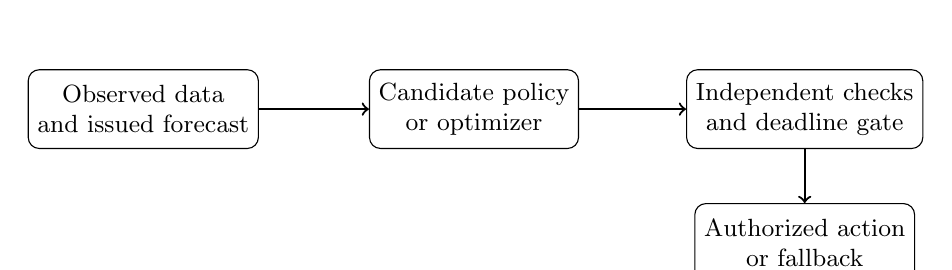
\begin{tikzpicture}[every node/.style={draw,rounded corners,align=center,font=\small,minimum height=1cm}]
\node (a) at (0,0) {Observed data\\and issued forecast};
\node (b) at (4.2,0) {Candidate policy\\or optimizer};
\node (c) at (8.4,0) {Independent checks\\and deadline gate};
\node (d) at (8.4,-1.7) {Authorized action\\or fallback};
\draw[->,thick] (a)--(b);\draw[->,thick] (b)--(c);\draw[->,thick] (c)--(d);
\end{tikzpicture}
\end{center}

\subsection{The trust chain}
A certificate proves something about an encoded instance and specification. The chain includes input identity, units, model construction, theorem or checking rule, arithmetic implementation, runtime environment, and physical actuation. Reducing the trusted code base can help, but it does not eliminate the need to validate sensors or model assumptions.

VIPR and LeanVIPR are concrete starting points for independently checkable mixed-integer linear programming certificates; their guarantees concern the encoded problem, not the complete power system.\cite{vipr,leanvipr} LP primal/dual witnesses can establish objective equality using exact arithmetic when rational data and witnesses are available. Floating-point solutions require justified reconstruction or interval bounds; rounding a dual vector can violate feasibility and invalidate a lower bound. For nonconvex OPF, a feasible point and a relaxation bound should be checked separately. For MILP, checking an incumbent is simpler than validating a global optimality claim; discrete proof artifacts and solver support differ.

Formal proofs of a controller's invariant can cover a bounded model and disturbance set. They do not establish that the real plant always stays within that set. Monitor envelope violations and make the fallback safe under the same timing and actuation assumptions.

\subsection{Deadlines and failure accounting}
Measure the complete path from observation availability to committed action, not just the optimizer's inner loop. Include parsing, preprocessing, data transfer, certificate generation, checking, and fallback selection. Report tail latency and missed deadlines alongside objective quality. A mean runtime below the sampling period is insufficient.

Treat timeout, infeasibility, numerical error, malformed input, and checker rejection as explicit outcomes. Score the resulting fallback trajectory, rather than dropping failed instances. A method can improve typical objective values while worsening service through rare failures. That tradeoff belongs in the main results.

\subsection{Independence must be designed}
Different implementations can share a model error; two kernels can check the same unintended theorem; two LLMs can share a reasoning pattern. Use separate formulations, dimensional checks, negative controls, known infeasible instances, and adversarial perturbations. Document shared dependencies. The VP/VNP audit is instructive because it distinguishes proof acceptance from statement correspondence and human understanding; the same distinctions apply to grid certificates.

\section{Work branch: preliminary experiments and null results}
\label{sec:results}
\status{Historical Work v0.2 executions; W03 reproduced W-E05 using its recovered code and inputs, but the original W-E01 and W-E04 remain historical reported results. Exploratory, deliberately small tests; no field deployment.}\cite{workbranch}

Work v0.2 reports that its separate evidence package contains the complete Python implementation, unmodified public PGLib case and license, generated BESS inputs, every hourly schedule, all AC starts, solver settings, and machine-readable results. The runs used Python 3.12.9, NumPy 2.2.4, SciPy 1.18.0, and macOS 27.0.1 on ARM. BLAS and OpenMP thread environment variables were set to one. These settings do not establish deterministic wall-clock performance or a hard real-time guarantee.

\subsection{W-E01: small AC-OPF, a null improvement result}
The case is PGLib-OPF v23.07 \texttt{case3\_lmbd}, downloaded at repository commit
\texttt{dc6be4b2f85c} (full hash in the results file). It has three buses and three branches, 315\,MW active demand, and a 100\,MVA base. The implementation uses polar voltages, fixes one reference angle, and optimizes two active and three reactive generator outputs. It includes branch charging, active and reactive balances, generator bounds, voltage limits, both-end apparent-power limits, and angle-difference bounds. It is a single-period AC-OPF, not security-constrained dispatch.

SciPy SLSQP minimized the quadratic generation cost divided by 10,000 for scaling, with \texttt{ftol}$=10^{-10}$ and at most 1,000 iterations. The first start uses unit voltage magnitudes and zero angles; nine additional starts perturb those quantities with seed 20261124. The comparator is the first start against the best of all ten. Multistart consumes more computation; it is not an equal-budget algorithm comparison.

A separate branch-by-branch reconstruction checks the final balances rather than using the optimizer's Y-bus residual function. The acceptance thresholds are $10^{-5}$\,MVA for balances and thermal violations, $10^{-5}$ degrees for angle violations, and $10^{-7}$ in the encoded variable-bound units. The two implementations still share the case interpretation and branch equations; independence is partial.

\begin{table}[ht]
\centering\begin{tabular}{lr}
\toprule W-E01 measurement & Result\\\midrule
Accepted solver outcomes &10 of 10\\
Feasible cost range (\$/h) &5812.642974235398--5812.642974235489\\
Active network loss (MW, approximately) &3.073200\\
Largest balance residual (MVA) &$6.93\times10^{-12}$ or less\\
Largest reported thermal/angle/bound violation &0\\
Per-start elapsed time, observed (s) &0.0306--0.0351\\
Analytic lossless lower bound (\$/h) &5638.967948718\\
Feasible objective minus lower bound (\$/h) &173.675025517\\
Relative bound interval, using feasible cost &2.9879\%\\
\bottomrule
\end{tabular}
\caption{W-E01 results from the recorded run. Timing is an uncontrolled local observation.}
\end{table}

The additional starts produce no material objective improvement: the full cost spread is below $10^{-9}$ dollars per hour. The case's own documented objective of approximately \$5812.64/h is a useful sanity comparison, not an independently replayed global-optimality certificate.

\textbf{Derivation of the lower bound.} Positive branch resistance and zero real shunts imply generation at least equals active demand. The two active-generator cost functions are increasing and convex over their nonnegative domain. Dropping network and reactive constraints and allowing total generation to equal demand therefore enlarges the feasible set. With costs $a_1p_1^2+b_1p_1+a_2p_2^2+b_2p_2$ and $p_1+p_2=D$, the interior minimizer is
\[
 p_1=\frac{2a_2D+b_2-b_1}{2(a_1+a_2)},\qquad p_2=D-p_1.
\]
The code checks nonnegative resistances and that these values lie within generator active bounds. The supplied case has zero constant cost terms. Evaluating this relaxed dispatch yields the stated lower bound. It is a bound for this encoded case; it is not a general-purpose AC relaxation implementation.

The \$173.675 interval includes network and loss restrictions removed by the bound. It is not a measured pool of savings. No new solver, learned cut, VP/VNP-derived algorithm, contingency analysis, or proof of global AC optimality was implemented.

\subsection{W-E05: storage service, loss, and baseline sensitivity}
The synthetic system has a 100\,MW import cap, 50\,MW charge and discharge limits, 200\,MWh maximum energy, 40\,MWh reserve floor, 100\,MWh initial energy, and final energy at least 100\,MWh. Charge and discharge efficiencies are each 0.95. Import ramping is limited to 20\,MW per hour, starting from 80\,MW. Time steps are one hour over a 24-hour horizon.

The balances are
\begin{align}
 g_t+d_t-c_t+u_t&=\ell_t,\\
 e_{t+1}&=e_t+0.95c_t-d_t/0.95.
\end{align}
Here $g$ is import, $d$ discharge, $c$ charge, $u$ unserved load, and $\ell$ requested load. Nonnegative $u_t\le\ell_t$ makes inadequacy explicit. These are constructed profiles, not measured data-center traces:
\begin{itemize}
\item Flat: 80\,MW throughout.
\item Four-hour peak: sixteen hours at 80\,MW, four at 140\,MW, four at 80\,MW.
\item Eight-hour peak: twelve hours at 80\,MW, eight at 140\,MW, four at 80\,MW.
\item Alternating: twelve hours at 80\,MW, four alternating 140/80\,MW pairs, then four hours at 80\,MW.
\end{itemize}

Three policies use the same physical limits. The simple threshold policy recharges only to the initial 100\,MWh target and shaves imports above the cap. The forecast-aware threshold charges toward 200\,MWh whenever a future above-cap peak remains, then restores the initial target. The lookahead LP uses the complete deterministic profile and lexicographically minimizes total unserved energy, then charge-plus-discharge throughput. The LP relaxation permits simultaneous charging/discharging in principle; every returned schedule was checked to have no simultaneous operation. This observed property is not asserted for arbitrary modified inputs.

\begin{table}[ht]
\centering\begin{tabular}{lrrr}
\toprule Unserved energy (MWh) & Simple threshold & Forecast threshold & LP\\\midrule
Flat &0&0&0\\
Four-hour peak &103&8&8\\
Eight-hour peak &263&168&168\\
Alternating &48.85&0&0\\\bottomrule
\end{tabular}
\caption{The apparent LP advantage disappears against the stronger policy comparator.}
\label{tab:bess}
\end{table}

Relative to the simple threshold, the LP serves an additional 95\,MWh in each continuous-peak case and 48.85\,MWh in the alternating case. Relative to the forecast-aware rule, it adds zero service on all four cases. The two stronger policies also have matching aggregate imports, throughput, losses, and terminal energy within floating-point tolerance. This ablation was added after the first comparison; the study is exploratory.

The improvement against the weaker comparator has an energy cost. In the four-hour peak case, storage conversion losses rise from 6.157895 to 16.421053\,MWh, and grid imports rise from 2063.157895 to 2168.421053\,MWh. Serving more demand is not synonymous with reducing energy losses. In the alternating case, losses rise from 12.007895 to 17.285319\,MWh while unserved load falls to zero. Work reports that its package records each balance and schedule so these conclusions can be checked directly.

\textbf{A physical lower bound is attained.} The continuous four-hour deficit above the import cap is $4\cdot40=160$\,MWh. The most that a fully charged device can deliver above its reserve floor is $0.95(200-40)=152$\,MWh. Equation~\eqref{eq:storagebound} therefore requires at least 8\,MWh unserved; both stronger policies attain it. The eight-hour deficit is 320\,MWh, leaving at least 168\,MWh unserved. Zero is the universal lower bound for the other two profiles, and it is attained. This establishes minimal unserved energy for these four specified profiles under the model; it does not establish a general policy theorem.

All twelve schedules passed energy, power-balance, bounds, ramp, terminal, and nonsimultaneity checks. The largest recorded numerical violation is below $10^{-12}$. The two-stage LP took approximately 0.0028--0.0109 seconds per profile in the recorded run. This is not a closed-loop MPC evaluation, a forecast-error test, a frequency or voltage study, an aging model, a revenue backtest, or a reliability accreditation study.

\subsection{W-E04: a small exact certificate and negative controls}
Consider the rational LP
\[
 \min 20x+50y\quad\text{subject to }x+y=100,\quad0\le x\le60,\quad y\ge0.
\]
The witness $(x,y)=(60,40)$ has objective 3200. The dual witness $(\lambda,\mu)=(50,30)$ obeys $\mu\ge0$, $\lambda-\mu\le20$, and $\lambda\le50$, with lower bound
\[
 100\lambda-60\mu=3200.
\]
Weak duality and equality certify this toy optimum under the stated rational model. The checker uses Python's \texttt{Fraction}; it accepts the witness and rejects four alterations: a capacity breach, a changed equality multiplier, a changed bound multiplier, and a demand-balance breach.

This is an exact-arithmetic demonstration, not a verified implementation of a checker, not a Lean proof, and not an AC-OPF or SCUC certificate. Four rejected mutations illustrate controls; they do not prove that every malformed certificate would be rejected. Its purpose is to demonstrate the candidate/witness/checker separation at a scale where every step is inspectable.

\subsection{VP-review checks reproduced}
In the Work branch, the supplied review's three Python scripts were copied with their required pinned transition-rule source, license, and notice. Work reports that their outputs were included separately from the grid benchmark results. Exact fraction checks reproduce the flat-branch numerical margin and the mixed-cut example; pointer enumeration exhausts its four finite examples; the cut script checks 16 expanded weighted terms and 15 resource cases. This reproduces selected diagnostics, not the paper's universal lemmas. The previous review's focused Lean outcomes remain \emph{reported historical executions}; no Lean compilation was performed for the Work edition or this integration.

\subsection{What was not run}
W-E02 (unit commitment/SCUC), W-E03 (converter MPC), and W-E06 (fleet economics and adequacy) were not executed by Work; the distinct Chat storage studies C-E002 and C-E003 were executed in its earlier research checkpoint. No ARPA-E GO full challenge, large PGLib suite, hardware-in-the-loop study, field pilot, or complete VP/VNP proof replay was run. This describes the historical v0.2 scope; W03 subsequently ran static AC-OPF, core UC, formal storage checking and forecast-control experiments (Section~\ref{sec:w03results}). Full security-constrained, converter and field studies remain unrun. Tables of expected outcomes or invented performance numbers are deliberately absent.

\section{W03: held-out experiments and machine-checked storage statements}
\label{sec:w03results}
\status{Work executed W03-A--E and a same-machine repeat on 24 November 2026. The original evidence package, report, source, input freezes and both runs are preserved. The present review verifies its integrity, replays selected recorded results, and reruns load control on Linux; it does not rerun all solver arms or rebuild Lean.}\cite{w03packet,w03review}

W03 changes the evidentiary standing of CRGC. It supplies formally checked storage statements and several constructive examples of representation-preserving reduction, but the primary comparisons fail to establish general solver superiority. Most importantly, a simpler forecast-aware control policy outperforms the tested rolling optimization on service. We separate three evidence levels: (I) representational equivalence or a certified restriction; (II) improvement in validated decision quality at a matched deadline against strong alternatives; (III) incremental operational service or real economic benefit at equal reliability. Only specific Level I results are established. Level II is inconclusive, and Level III is not established. These levels are not a progression that every result automatically satisfies.

\subsection{W03-A: adaptive heterogeneous storage under deadline}
The one-hour model minimizes import expenditure plus linear throughput cost, with individual efficiencies, energy limits, availability, terminal conditions and mutually exclusive modes. Using the symbols in Section~\ref{sec:compression}, for the tested finite horizon,
\[
 J=\sum_t\left(\lambda_t g_t+\sum_i k_i(c_{it}+d_{it})\right),\qquad
 e_{i,t+1}=e_{it}+\eta_{ci}c_{it}-d_{it}/\eta_{di}.
\]
Grid balance, import limits and ramps are common to all policies. Fixed proportional allocation is a stronger restriction than sharing charge/discharge modes while retaining individual allocations. A checked common fallback is available for each instance, including the forced-opposition cases.

The design, frozen before the held-out panel, uses eight development instances and two held-out seeds (7301, 8297), three sizes (4 devices by 8 hours, 8 by 12, 12 by 16), and four cohorts: ordinary heterogeneous, negative-price/outage/reserve, interchangeable, and forced opposing modes. Three repeats across each eligible policy give 450 total trials (the symmetry arm applies only to interchangeable cases). The original single-threaded ARM64 Mac trials include fallback validation, model building, presolve, solving, reconstruction and validation within the two-second clock. Target attainment requires a validated unrestricted feasible incumbent $U$ and a full-model lower bound $L$ such that
\[
 U-L\le 2\times10^{-5}+10^{-3}\max(1,|U|).
\]
Report the original target convention even when $U$ is near zero or negative. A grouped model's own lower bound cannot be substituted for the unrestricted lower bound. The original MILP dual bounds remain numerical, not exact certificates.

\begin{table}[htbp]\centering\small
\caption{W03-A case-level target attainment: all three repeats must hit within two seconds. Each cohort contains six constructed cases. Source: W03 report pp. 2--3 and \texttt{results/A/cohorts.csv}.}\label{tab:w03a-hits}
\begin{tabular}{lrrrr}\toprule
Cohort & Full LP & Full MILP & LP recovery & Adaptive\\\midrule
Ordinary heterogeneous &6&6&6&6\\
Negative price/outage &6&6&6&6\\
Interchangeable &6&6&6&6\\
Forced opposition &0&2&2&2\\\midrule
Total &18&20&20&20\\\bottomrule\end{tabular}
\end{table}

The adaptive policy accepts the LP directly on the first 18 cases. On all six forced-opposition cases, at least one raw LP device charges and discharges simultaneously; the single shared-mode root is infeasible. Intermediate groups produce feasible improvements, but no grouped stage reaches the prescribed unrestricted gap. The unrestricted MILP eventually supplies the adaptive policy's final winning schedule on all six. The two 4-device forced cases reach the target; the other four do not in either arm. LP sign repair followed by unrestricted recovery reaches the same two targets. Fixed proportional control produces higher returned cost on all 12 ordinary and negative-price cases and is infeasible on four of six forced cases. Symmetry breaking on the interchangeable cohort is slower by the reported median capped time (74.75 ms versus 26.85 ms for the full MILP). These comparisons are not population estimates.

\begin{table}[htbp]\centering\small
\caption{Forced opposition: original median time to first strictly improved validated fallback (ms), not time to matched-quality dispatch. Source: W03 report p. 3.}\label{tab:w03first}
\begin{tabular}{lrrr}\toprule
Devices $\times$ hours & Seed & Full MILP & Adaptive\\\midrule
$4\times8$ &7301&48.47&101.13\\
$4\times8$ &8297&104.68&23.23\\
$8\times12$ &7301&332.72&161.69\\
$8\times12$ &8297&317.72&44.25\\
$12\times16$ &7301&888.67&276.78\\
$12\times16$ &8297&1,134.42&43.39\\\bottomrule\end{tabular}
\end{table}

The secondary endpoint favors the adaptive policy in five of six forced cases, but the first improved incumbents can have materially different costs. In the current retrospective analysis we reconstruct $U_m(t)$ as the best recorded feasible cost available by elapsed time $t$ for method $m$, retaining the common fallback. Within each case take the median over three repetitions and compare costs using an absolute $10^{-5}$ tie tolerance. Table~\ref{tab:w03frontier} is a more direct view of the deadline-conditioned value frontier. It is post hoc, not a preregistered test, and uses recorded clocks rather than newly measured timing.

\begin{table}[htbp]\centering\small
\caption{Adaptive incumbent cost at fixed deadlines: six forced-opposition cases, better/tied/worse. Recomputed from W03 event logs. Equal final costs do not imply equal time to reach the target.}\label{tab:w03frontier}
\begin{tabular}{lcc}\toprule
Elapsed deadline & versus full MILP & versus LP recovery\\\midrule
50 ms &3 / 2 / 1&3 / 3 / 0\\
100 ms &3 / 2 / 1&3 / 2 / 1\\
250 ms &3 / 2 / 1&3 / 2 / 1\\
500 ms &2 / 2 / 2&2 / 2 / 2\\
1 s &1 / 2 / 3&1 / 2 / 3\\
2 s &0 / 6 / 0&0 / 6 / 0\\\bottomrule\end{tabular}
\end{table}

This narrows the credible candidate mechanism: a grouped solve may be a primal heuristic to create a useful incumbent, not a substitute for a strong unrestricted optimizer. Repeated sequential restriction solves may consume the remaining deadline. W04-A tests grouped warm starts against a full solver supplied with an LP-informed warm start or repair under identical end-to-end budgets. A tie in target attainment with no matched-quality advantage over LP recovery is not a positive solver claim.

\subsubsection{Exact LP lower bounds and validation scope}
For a minimization LP with finite variable box $\ell\le x\le u$ and row bounds $a\le Ax\le b$, choose a multiplier vector $y$ with zero components for unavailable selected row sides. Define $r=c-A^\top y$ and
\[
 L(y)=\sum_{j:y_j>0}y_j a_j+\sum_{j:y_j<0}y_j b_j
 +\sum_{i:r_i>0}r_i\ell_i+\sum_{i:r_i<0}r_i u_i.
\]
For any feasible $x$, each row term is at most $y^\top Ax$ and each residual term is at most $r^\top x$, giving $L(y)\le c^\top x$. A full-model LP relaxes integrality, hence its lower bound applies to the full MILP. W03 reconstructs these expressions using exact rational interpretations of the stored binary64 coefficients. The independent review recalculated all 24 witnesses and reproduced the exact recorded bounds. This certifies the encoded LP box bound, not the intended continuous physical system without coefficient/units and model correspondence review. The archive's MILP solver dual bounds are not exact rational certificates.

\subsection{W03-B: formal storage theorems and counterexamples}
The supplied \texttt{formal/Storage.lean} compiles in the recorded Work environment against Lean \texttt{4.30.0-rc2} and mathlib commit \texttt{896cc56a395e1615786fac56564a3fe6bfeebcc4}. The recorded dependency inspection reports no tracked modifications; dependencies were prebuilt, not rebuilt. Sixteen named declarations have axiom reports listing standard logical axioms (\texttt{propext}, \texttt{Classical.choice}, \texttt{Quot.sound}, as applicable); no \texttt{sorryAx} dependency is reported. The present review inspected the statements and logs and reran finite exact controls, but has not independently rebuilt the Lean dependency closure. State the result as machine-checked in the recorded environment, not as a new local kernel replay. Four concrete false control statements failed compilation; a small rational certificate accepts its valid witness and rejects four corruptions. These do not establish completeness of a general-purpose checker.

\paragraph{Balanced lift and threshold equivalence.} For $N>0$, let $q=\lfloor S/N\rfloor$, $r=S\bmod N$, and $b_i(S)=q+\mathbf{1}_{i<r}$ for $0\le i<N$. This is the earlier floor convention with one fixed reversal of labels. The checked lemmas include total energy $\sum_i b_i(S)=S$, capacity when $S\le NC$, translation $b_i(S+NR)=b_i(S)+R$, monotonicity and per-member rate bounds. They imply $\sum_i|b_i(U)-b_i(S)|=|U-S|$. For a full labeled trajectory $x$ and total $s(t)=\sum_i x(t,i)$, let $\mathcal F$ be the ideal integer storage feasible set with individual capacity $C$, symmetric rate $R$, and prescribed balanced endpoints $b_i(A)$ and $b_i(B)$ in the same labeling. Let $\mathcal G$ be the total-energy trajectories with capacity $NC$, rate $NR$ and endpoints $A,B$. Any external constraint or fee $F$ may depend on the complete aggregate trajectory, not on individual unrepresented obligations. Let $k\ge0$ be a common real linear movement cost. Work's \texttt{same\_threshold\_real} proves, for every real threshold $\beta$,
\begin{align}
 &\exists x\in\mathcal F:\quad F(s)+k\sum_{t,i}|x(t+1,i)-x(t,i)|\le\beta\nonumber\\
 &\hspace{5mm}\Longleftrightarrow\quad
 \exists s\in\mathcal G:\quad F(s)+k\sum_t|s(t+1)-s(t)|\le\beta .\label{eq:w03threshold}
\end{align}
The projection direction uses the triangle inequality; the balanced lift preserves cost exactly in the reconstruction direction. This formulation handles infeasibility as well as equal optimal values. It does not guarantee that every original path can be reconstructed from its total, nor does it assert that any balanced labeling can be changed between endpoints. For example, $(1,0)$ to $(0,1)$ has constant total but incurs two units of labeled movement; a zero-cost aggregate path cannot realize that required swap. The theorem's scope is a discrete ideal model, not arbitrary batteries, heterogeneous AC-side conversion, or operationally validated site control. Work reports 27,776 finite balanced-lift transition checks.

\paragraph{Unequal efficiency obstruction and tolerance.} The checked statements \texttt{no\_common\_cycles} and \texttt{two\_device\_bound} lift the earlier arithmetic to finite-horizon SOC dynamics. For positive weights $w_i$, nonnegative common charge $C_t$ and discharge $D_t$, and time-invariant discharge efficiency $\eta_{di}>0$, write $\rho_i=\eta_{ci}\eta_{di}$. The per-period equation, after clearing the denominator, is
\[
 \eta_{di}(e_{i,t+1}-e_{it})=w_i(\rho_i C_t-D_t).
\]
Telescoping gives $\rho_i\sum_t C_t-\sum_t D_t=\eta_{di}(e_{i,T}-e_{i,0})/w_i$. Exact cyclic endpoints and $\rho_i\ne\rho_j$ force the two common sums to zero; nonnegativity forces every $C_t,D_t$ to vanish. If the endpoints instead obey $|e_{i,T}-e_{i,0}|\le\delta_i$, then
\begin{equation}
 |\rho_i-\rho_j|\sum_t C_t\le \frac{\eta_{di}\delta_i}{w_i}+\frac{\eta_{dj}\delta_j}{w_j}.
 \label{eq:w03tolerance}
\end{equation}
This is a necessary throughput bound, not a sufficient condition for feasibility. The exact rational example $\sum C=1$, $\sum D=4/5$, $\rho_i=4/5$, $\rho_j=81/100$, equal weights $1/2$, discharge efficiencies 1 and $9/10$, and terminal deviations $0,1/180$ attains both sides at $1/100$. Thus a positive terminal interval can allow nonzero throughput, even with unequal efficiency. The proof does not verify the optimizer, plant, thermal/degradation model, tariff, or VP/VNP.

\subsection{W03-C: exact local variable elimination in static AC-OPF}
At a generator bus $i$, the power balances can be written $\sum_{g\in G_i}P_g=P_i(V)+P_i^d$ and similarly for reactive power (with shunt and transformer conventions retained in the model). Select a generator $g_i$ whose two balance coefficients are unity. Substitute
\begin{align*}
 P_{g_i}&=P_i(V)+P_i^d-\sum_{g\in G_i\setminus\{g_i\}}P_g,\\
 Q_{g_i}&=Q_i(V)+Q_i^d-\sum_{g\in G_i\setminus\{g_i\}}Q_g.
\end{align*}
Keep its original limits and cost on these expressions, along with every other constraint. Then projection deleting these variables and substitution back are inverse on the original feasible set; objective values are identical. This elementary elimination is exact for the specified static representation. It is not a consequence of the VP/VNP theorem or a claim of novel AC optimization. It may increase coupling in derivatives or worsen conditioning. A global optimizer is not established merely by recovering matching local solutions.

The pinned public PGLib normal and active-power-increase cases span 5, 14 and 30 buses. Three arms (full flat start, full DC-informed start, elimination with the same retained-voltage DC start) use IPOPT with automatic sparse derivatives; settings were selected on the 3-bus development instance. The generator initialization implied by elimination may differ from the full DC start. Two repeats per arm/case and a 12-second deadline yield 36 returns, all independently checked within the stated tolerances in the archived run. A fresh replay using the delivered branch-end checker accepted all 36 and rejected all 36 corrupted injections. The maximum median objective difference within a case is under $2\times10^{-6}$ dollars per hour. The lower estimates from lossless dispatch and the local solver do not prove global optimality.

\begin{table}[htbp]\centering\small
\caption{W03-C. Positive elapsed differences favor the full DC-start model; negative favor elimination. Two repeats per arm. Source: W03 report p. 5 and \texttt{results/C/comparison.csv}.}\label{tab:w03ac}
\begin{tabular}{lrrr}\toprule
Network & Variables full/reduced & Normal cost (\$/h) & Elimination time difference (ms)\\\midrule
5-bus PJM &20/12&17,551.89&$+0.92$ / $+0.28$\\
14-bus IEEE &38/28&2,178.08&$-0.66$ / $+0.42$\\
30-bus IEEE &72/60&8,208.52&$-0.23$ / $-1.12$\\\bottomrule\end{tabular}\par\footnotesize Time differences are normal / stressed variants; stressed costs were 78,949.91, 5,999.36 and 18,036.59 \$/h, respectively.
\end{table}

The declared variable reductions (40.0\%, 26.3\%, 16.7\%) do not establish a consistent runtime advantage. W04-C extends the network scale and measures derivative/KKT sparsity, symbolic factorization fill, conditioning diagnostics, and end-to-end feasible cost and timing. These are static AC-OPF experiments, not security-constrained operation.

\subsection{W03-D: permanent generator pairing is a costly restriction}
The PGLib-UC reference preserves initial histories, minimum up/down times, ramp, reserve, piecewise costs, startup and renewable availability. Pairing ties on/off decisions of similar units with matching minimum-time, must-run and initial-status categories, while preserving individual physical constraints. The test includes two fleets and 12-hour prefixes (later obligations excluded) versus native 48-hour instances, under a nominal 45-second end-to-end gate. It is UC without transmission or contingencies, not SCUC.

\begin{table}[htbp]\centering\small
\caption{W03-D primary run: benchmark cost units, not field savings. All no-incumbent arms retained. Source: W03 report p. 6.}\label{tab:w03uc}
\begin{tabular}{lrrr}\toprule
Case & Full feasible & Paired feasible & Increase\\\midrule
RTS 12 h &228,050.56&230,790.61&1.20\%\\
RTS 48 h &2,516,915.98&2,532,321.68&0.61\%\\
California 12 h &9,322.20&9,441.22&1.28\%\\
California 48 h &--&--&No incumbent\\\bottomrule\end{tabular}
\end{table}

For the two 12-hour instances the paired restriction's solver-reported lower bound exceeds the full model's feasible incumbent. Thus, conditional on numerical bound validity, even the best restricted schedule is worse than an already feasible unrestricted schedule by at least 1,683.71 (RTS) or 118.47 (California) cost units, rounded down. These different instances must not be added. At 48 hours the RTS bounds overlap; only returned-schedule differences are supported. The California 48-hour instance has no feasible incumbent in either arm, and the reference solver overran the overall deadline at 56.19 seconds; no feasible fallback was available. Six archived schedules passed Work's checks, but this review has not rebuilt the UC models locally. The same-machine repeat reproduced eight deadline classifications while some costs changed within gap/time limits. Permanent pairing is not supported; W04-D tests temporary pairing as a warm-start heuristic only.

\subsection{W03-E: forecast rule versus finite-horizon rolling optimizer}
The W-E05 historical panel is reproduced in the W03 packet: forecast-aware threshold and LP tie in all four profiles, with unserved energy $0,8,168,0$ MWh. W03 adds eight latent synthetic days, reused across three regimes (ordinary, biased forecast, outage and reserve). Both online policies see the same current load, six-hour issue-time forecast and one-hour outage notice. They share 100 MW import cap, 23 MW/h ramp, 35 MW / 180 MWh battery, nonideal efficiency, a late-day floor enforcing at least 95 MWh terminal energy, and 24 MW fixed facility demand. Flexible computing service is modeled as served electrical MWh, not completed jobs or revenue. The rule holds a precautionary 95 MWh target and precharges for forecast deficits; the rolling LP first minimizes six-hour unserved energy, then minimizes throughput, with no continuation value beyond the horizon. The offline 24-hour model has perfect foresight and is a bound/comparator for its stated objective, not a deployable policy.

\begin{table}[htbp]\centering\small
\caption{W03-E original primary run, sum of unserved MWh over eight synthetic days per regime; rolling wins/ties/losses versus forecast rule. Source: W03 report p. 7.}\label{tab:w03e}
\begin{tabular}{lrrrr}\toprule
Regime & Rule & Rolling & Offline & W/T/L\\\midrule
Ordinary &422.95&471.26&212.37&0/1/7\\
Biased forecast &479.93&545.33&212.37&0/0/8\\
Outage and reserve &628.76&693.01&575.57&0/3/5\\\midrule
Total &1,531.64&1,709.61&1,000.30&0/4/20\\\bottomrule\end{tabular}
\end{table}

The forecast rule serves 177.967806 MWh more than the rolling policy in the original panel, while rolling uses less throughput and conversion loss in every regime total. No online fallback was invoked. In the outage regime all three policies lose 128 MW-hours of contracted headroom availability across eight days; energy reserves do not restore unavailable inverter power. The two policies differ in both precautionary energy valuation and planning rule, so a terminal-value or horizon effect is a hypothesis, not an identified cause.

The present Linux replay uses the frozen inputs and the delivered \texttt{load\_control.py} simulation (Python 3.13.5, SciPy 1.17.0, NumPy 2.3.5), with no new tuning or forecast generation. All 72 policy/day simulations ran without fallback. The rolling policy again wins none, ties five and loses nineteen; the forecast rule serves 176.069173 MWh more. Exactly one material difference in unserved energy was found at tolerance $10^{-6}$ MWh: rolling MPC on \texttt{outage\_reserve\_864} changes from 59.274810 to 57.376177 MWh unserved. Different solver versions or selection among alternative intermediate optima are possible explanations; no cause was established. The original and replay remain separate, not averaged or silently reconciled. This motivates deterministic tie-breaking (and reporting service as the primary lexicographic quantity) plus a factorial continuation-value and horizon ablation on fresh days. A lower cycling cost is not a service improvement, and the service outcome is not measured computing goodput.

\subsection{Review provenance and remaining obligations}
The supplied W03 report is byte-identical to the enclosed PDF; all 86 listed file hashes pass. The read-only reviewer script and machine-readable outputs are distributed as the companion v0.3 review archive. A fresh run checked the 450 policy records for denominator and reported target consistency, 367 saved battery candidates and incumbents (including rejected schedules), exact LP bounds for all 24 instances using the delivered matrix construction and rational evaluator, 36 archived AC solutions and 36 mutation controls using the delivered independent checker, and 1,728 archived site-policy hourly actions with a separate trajectory calculation. The review independently recalculated the fixed-deadline incumbent comparisons and reran 72 site-policy simulations. The battery and load validation code checks the recorded physical constraints; it is not external utility validation. Work's same-machine replay and this partial cross-platform replay are not additional independent instance populations.

\begin{table}[htbp]\centering\small
\caption{Evidence scope of the W03 review. A logged build and a fresh kernel rebuild are distinct.}\label{tab:w03review}
\begin{tabularx}{\linewidth}{Y Y}\toprule
Evidence checked & Remaining scope limitation\\\midrule
86 manifest hashes; 450 records; 367 A schedules; 24 exact LP box bounds & No fresh 450-trial MILP benchmark; solver dual gaps not rational certificates.\\
Lean source, axiom logs, proof hypotheses and exact controls & No independent full Lean/mathlib build. No optimizer or plant verified.\\
36 archived AC feasibility/cost checks and 36 corrupted vectors & No fresh larger OPF or global optimality.\\
Six UC schedules and two misses reported by Work & No independent UC reconstruction/solver rerun in current environment.\\
1,728 archived E actions; 72 fresh E simulations & One environment-dependent scenario; no field trace or population estimate.\\\bottomrule\end{tabularx}
\end{table}

The present review does not use its partial replays as evidence of overall mathematical novelty or commercial grid value. W03 strengthens H2 against the broad H1 interpretation: the LP already resolves many cases, permanent grouping can be costly, and a simple policy can beat the rolling optimizer. H3 remains a candidate for a narrower deadline-dependent primal-heuristic contribution. No quantified probability or general population conclusion follows from these constructed panels.


\section{W04: reconstruction guarantees, rejected compression mechanisms and predictive control}
\label{sec:w04results}
\status{Executed Work campaign, 24 November 2026. Findings below are sourced to the supplied original W04 report and prior Chat review. Review is scoped to stored evidence and arithmetic; no independent complete W04 solver campaign or full Lean rebuild.}\cite{w04packet}

\subsection{Experimental contract and evidence architecture}
W04 uses common constraints, information, budget and validation within each comparison. Track A comprises 72 constructed battery cases, five policies and three rotated repeats. Track B reports formal declarations and finite checks. Track E comprises 24 latent days, each in three paired regimes, and twelve policy/reference paths per scenario-day. Track C comprises four public AC cases in two variants, four formulations and five repeats. Track D comprises three UC dates at two horizons, four arms, and a separate serial sensitivity. Timings are from a shared eight-logical-CPU ARM64 Mac with one solver thread; unrelated work and concurrent campaign activity contended for the host. The gates are 2 s (A), 1 s per simulated decision (E), 12 s (C), 45 s (D). A validated terminal result arriving after the gate receives no on-time credit. W04 has no independent second-machine operational replication.

The prior Chat review reports all 743 entries in the W04 integrity manifest passed, and the standalone TeX matched the archived copy. It independently recalculated 3,019 battery witnesses, 1,080 deadline classifications from logs, 160 archived AC vectors and 160 imbalance perturbations, 864 load trajectories and 20,736 hourly actions. Exact arithmetic controls were reproduced. These are archival witness and arithmetic checks, not fresh timing trials or kernel builds. Source report and archive are retained in the research workspace; separate reviewer code from that review has not been attached to this checkpoint. Distinguish original, repeat, reanalysis and prospective results.

\subsection{W04-A: grouped warm starts versus LP-informed recovery}
W04 tests temporary inner restrictions, transferring validated incumbents into the unrestricted MILP. LP repair uses relaxation signs with partial fixing fallback; a grouped-search ablation retains its best checked candidate but starts unrestricted recovery from the common fallback. The candidate-generation time budget (30\% of 2 s) was selected on W03 development cases. A hit requires $U-L\le 0.00002+0.001\max(1,|U|)$, with $U$ checked against original constraints and $L$ an unrestricted bound. A case hits only if all three repeats hit.

\begin{table}[htbp]\centering\small
\caption{W04-A, target hits by cohort. Each cohort has 18 constructed cases; total 72. Source: W04 report, A section.}
\begin{tabular}{lrrrrr}\toprule
Cohort & Full MILP & Raw LP & LP repair & Group start & Ablation\\\midrule
Ordinary &14&18&18&18&18\\
Negative price/outage &17&18&18&18&18\\
Forced opposition &0&0&0&0&1\\
Interchangeable &14&18&18&18&18\\\midrule
Total &45&54&54&54&55\\\bottomrule
\end{tabular}
\end{table}

All 54 successful LP-repair and grouped-start cases accepted the already-admissible raw LP at the first stage. Therefore the nine additional hits relative to direct full MILP do not identify a grouping contribution. All 18 forced root restrictions are infeasible in separate presolve diagnostics. At 2 s the group-start method has 5/11/2 practical wins/ties/losses versus direct MILP, but 0/11/7 versus LP repair. At 250 ms the corresponding group versus LP-repair comparison has 1/8/8 on 17 paired cases; one early comparison is missing. The practical threshold is 0.1\% of $\max(1,|U_{\rm fallback}|)$. The forced-cohort paired median normalized incumbent-cost integral is 0.258 worse than LP repair (six-seed block bootstrap interval 0.164--0.289). A transferred start and a downstream improvement are different endpoints: HiGHS acknowledged 31 nonfallback grouped starts among 54 recoveries and 37 among 53 LP-informed recoveries. The transfer ablation prevents attributing all retained candidates to the warm start.

Of 1,080 trials, 234 returned after 2 s (maximum 4.773 s); late improvements were excluded. The report records 72 exact LP box witnesses and 144 corruptions, with accepted physical residual below $8.51\times10^{-12}$ in checked units. Exact rational evaluation applies to the stored binary64 coefficients interpreted as rationals, not unknown real device parameters. The forced cases are intentionally constructed; their 18/72 frequency is not a field prevalence estimate.

\textbf{Disposition.} Retire the tested grouping-superiority claim. Preserve the code as a negative comparator. Advance a narrower screening question: when does checking an unrestricted relaxation and escalating only if required outperform a strong native solver and LP recovery at the same quality and complete deadline? This is established optimization practice, not a newly discovered general algorithm. A smaller model does not establish easier search.

\subsection{W04-B: exact thresholds and sharp bounded regret}
\label{sec:w04math}
Let $X,Y$ be feasible domains with real costs $J,K$. For every real threshold $b$, define $T_J(b):=\exists x\in X:J(x)\le b$ and $T_K$ analogously. If total maps $p:X\to Y$ and $f:Y\to X$ satisfy
\[
 K(p(x))\le J(x),\qquad J(f(y))\le K(y),
\]
the two witness directions establish $T_J(b)\iff T_K(b)$, including the case where both domains are empty. If only a returned minimizer $\hat y$ has a validated feasible lift $\hat x$, the chain $J(\hat x)\le K(\hat y)\le K(p(u))\le J(u)$ for all $u\in X$ proves attainment at $\hat x$. Equal infima without a lift do not establish attainment; compare $(0,\infty)$ with $[0,\infty)$ under identity cost.

For nonempty domains with finite infima $j=\inf J(X)$ and $k=\inf K(Y)$, assume the uniform projection inequality $K(p(x))\le J(x)+\alpha$ for every $x$. If $K(\hat y)\le k+\epsilon$ and one verified feasible lift obeys $J(\hat x)\le K(\hat y)+\beta$, then
\begin{equation}
 0\le J(\hat x)-j\le\alpha+\beta+\epsilon .
 \label{eq:w04sharp}
\end{equation}
Here $\alpha,\beta,\epsilon\ge0$ are cost-unit errors, and no global lift is necessary for this candidate bound. The full two-sided infimum sandwich $k-\alpha\le j\le k+\beta$ additionally requires the lift inequality for every reduced point or equivalent control of its infimum. Uniform projection cannot be established from a finite simulation panel.

Sharpness: take two feasible points in each space. Give the full points costs $0,\alpha+\beta+\epsilon$ and reduced points costs $\alpha,\alpha+\epsilon$. Project both full points to the first reduced point; lift by matching labels. The two transfer inequalities hold. Returning the second reduced point attains regret $\alpha+\beta+\epsilon$. Thus the universal constant cannot improve without extra hypotheses. This is a simple conditional mathematical result, not a claim of priority or a performance theorem.

W04 reports Lean 4.30.0-rc2 checked 32 new declarations plus the historical 16, with eight false statements rejected, nine pinned dependency checkouts, and transitive axiom reports limited to the standard logical axioms or subsets. The recorded exact controls include 1,296 map/objective combinations and 2,592 candidate inequalities, plus the prior balanced-storage controls. The compiler and dependencies are part of the trusted base. The prior Chat review reports arithmetic reproduction and proof-source inspection, not an independent rebuild. No theorem establishes optimizer implementation correctness, physical-model validity or runtime improvement.

\subsection{Constructive candidate for W05: feasible convex-slice repair}
\label{sec:repair}
\status{Historical v0.4 derivation; W05 subsequently reports formal checks and engineering falsification of the near-optimality claim. See Section~\ref{sec:w05results}. No geometric novelty claim.}
The W04 result is most valuable if $\alpha$ and $\beta$ can be computed without solving the original problem. A candidate reconstruction certificate is the following elementary convex-repair construction.

Let the full continuous slice be $X=\{x\in B: Ex=d,\ Ax\le b\}$ where $B$ is convex, $E,A$ are finite matrices, and $x_0\in X$ is an independently validated anchor. Let a tentative reconstruction $\tilde x\in B$ satisfy $E\tilde x=d$, but possibly violate inequalities. For each row set
\[
 \delta_i=(A_i\tilde x-b_i)_+,\qquad
 \sigma_i=b_i-A_ix_0\ge0.
\]
Define $\lambda=0$ if every row is satisfied; otherwise
\[
 \lambda=\max_{i:\delta_i>0}
       \frac{\delta_i}{\delta_i+\sigma_i},\qquad
 x^+=(1-\lambda)\tilde x+\lambda x_0.
\]
Since $0\le\lambda\le1$, convexity gives $x^+\in B$ and linearity preserves the equalities. For any previously violated row,
\[
 A_i x^+-b_i=(1-\lambda)\delta_i-\lambda\sigma_i\le0.
\]
All other rows remain feasible by convexity. Thus $x^+\in X$. A violated row with zero anchor margin forces $\lambda=1$, so the construction returns the anchor rather than claiming a nontrivial repair.

For affine cost $J$, the reconstruction cost difference is exactly
\[
 J(x^+)-J(\tilde x)=\lambda[J(x_0)-J(\tilde x)].
\]
For an $L_J$-Lipschitz objective on $B$ with $\|x_0-\tilde x\|\le D$, the nonnegative repair loss is bounded by $L_JD\lambda$. If all violated rows have $\sigma_i\ge\sigma>0$ and $\delta_i\le\bar\delta$, a uniform bound over those candidates is
\begin{equation}
 [J(x^+)-J(\tilde x)]_+\le L_JD\frac{\bar\delta}{\bar\delta+\sigma}.
 \label{eq:repairbound}
\end{equation}
If $J(\tilde x)\le K(\hat y)+\eta$ is independently justified, the lift error for this candidate can be bounded by $\beta=\max(0,\eta)+L_JD\lambda$. A uniform projection bound and reduced quality guarantee remain separate obligations in Equation~\ref{eq:w04sharp}. An unrestricted bound $L$ also yields the direct feasible-incumbent certificate $U-j\le U-L$.

For illustration only, take $B=[0,4]^2$, $x+y=4$, $x\le2.5$, $y\le3.5$, anchor $(2,2)$, and tentative $(3,1)$. The violated row has $\delta=\sigma=0.5$; hence $\lambda=1/2$ and the repaired point is $(2.5,1.5)$. With $J=-x$, repair increases the tentative cost by 0.5. This is a hand-worked exact example, not an executed benchmark.

\textbf{Boundaries.} Convex mixing does not repair an equality residual except by returning the anchor; an equality correction requires a separate checked argument. If the problem is mixed-integer, both points must belong to the same integral mode slice (or another proved convex feasible subclass); averaging different binary modes is not a feasible MIP lift. A nonconvex AC feasible set does not satisfy the needed convexity. A zero-slack anchor may eliminate all useful repair. The cost of finding an anchor, computing margins, reconstruction and verifying original constraints belongs to the deadline. W05 should compare this bound to fixed-mode repair LPs, polytope disaggregation and existing approximate aggregation literature, and seek useful storage-specific endpoint corrections with ramp, reserve, availability and efficiency constraints. An abstract inequality is not evidence of practical performance.

\subsection{W04-C: exact AC elimination and the numerical cost of representation}
At a generator bus, eliminate one online unit's active/reactive outputs using the local balance equalities; retain its original objective and limits, both branch-end thermal limits and the remaining model. This is exact substitution on the common implemented static AC formulation, not a VP/VNP-derived optimization algorithm. W04 uses 57-, 118-, 300- and 1,354-bus PGLib networks in normal and active-power-increase variants. Four arms compare full DC, full matched, all-pivot and selective-pivot formulations. All 160 terminal vectors passed physical checks, 147 passed within the gate; accepted costs match the published reference at its printed precision. No global optimality follows. The 12-second pass counts are 36,37,37,37 of 40 per arm; neither elimination policy reaches the prespecified 10\% median speed improvement on any case against either full start.

\begin{table}[htbp]\centering\small
\caption{W04-C, 1,354-bus typical: full DC versus all-pivot structural diagnostics. Elapsed ratio compares matched full start.}
\begin{tabular}{lrr}\toprule
Quantity & Full & All-pivot\\\midrule
Decision variables &3,228&2,708\\
Jacobian nonzeros &39,526&39,006\\
RCM added lower-factor entries &99,221&107,615\\
Constraint rows &8,681&8,681\\
Hessian entries &19,096&19,096\\
Regularized KKT condition proxy &$6.43\,10^{12}$&$4.55\,10^{12}$\\\bottomrule
\end{tabular}
\end{table}

The recorded all-pivot/matched-full median elapsed ratio is 1.096 on three matched on-time repeats in this network/variant. Fewer variables coexist with approximately 8.5\% greater symbolic added fill; the regularized one-norm proxy improves. Symbolic RCM and SuperLU/COLAMD diagnostic estimates are not IPOPT's actual factorization. This establishes the importance of separate representation size, numerical sparsity/conditioning, and complete execution time. It does not identify a causal speed predictor from one case.

The source reports extra individual angle boxes $|\theta_i|\le2\pi$ are proved redundant only at 57 and 118 buses; retain them in all arms or establish redundancy independently. All eight cases have linear active costs and a single online unit at each generator bus; quadratic costs and multi-generator coupling remain untested. The frozen reduced-start diagnostic erroneously reads original DC generator values; actual reconstructed starts showed up to roughly 947 MW/MVAr component violation in the largest typical all-pivot case. The matched full initialization controls only all-pivot, not every selective arm. W05-C must fix these comparisons before claiming a selection advantage.

\subsection{W04-D: temporary unit grouping and supervisory failures}
W04 compares the full PGLib-UC MILP, LP-informed repair, temporary grouped-start recovery restoring all unit statuses, and permanent restriction across three dates and two horizons. These are core UC models, not network-contingency SCUC. The primary panel suffers 20/24 worker kills, including 18 before a first checkpoint. One grouped-arm schedule is returned, without a grouped start; on the single jointly evaluable group/LP case its cost is 0.141\% higher. The primary panel cannot isolate transfer effects.

The whole-panel serial sensitivity uses one UC lane and longer import allowance; it is post hoc and must not replace or be pooled with the primary run. All four methods return schedules on the same five of six cases, with none on California 48 h. Full, LP repair and grouped recovery each meet four of six numerical targets; permanent grouping meets zero. Grouping costs more than LP repair on all five comparable serial cases, materially so on three under the 0.1\% criterion. UC bounds are solver-reported numerical estimates, not independently constructed exact dual certificates. Retire this grouping strategy pending a substantively new, predeclared mechanism. Retain startup failures as evidence about end-to-end execution, not about mathematical infeasibility.

\subsection{W04-E: decision policy, continuation value and forecast horizons}
\label{sec:w04control}
The simulated facility has a 35 MW/180 MWh battery, a fixed facility load and flexible computing demand, 100 MW import cap, ramp, reserve headroom, SOC floor and terminal recharge. Each issue time has a frozen forecast up to 12 hours; shorter policies see only the corresponding prefix. Current load, one-hour outage notice and shared reserve calendar are provided. The actual continuation policy first minimizes forecast shedding, then end-of-window shortfall relative to a precautionary target, then throughput, with a deterministic first-action tie-break. It is not a general scalarized MPC value-function solution. The target uses a development-estimated 75th percentile of a six-hour future net-energy-draw statistic, capped at physical energy capacity; it omits some ramp/uncertainty interactions. The comparator receives the same horizon prefix.

\begin{table}[htbp]\centering\small
\caption{W04-E, paired continuation minus comparator, unserved flexible MWh per scenario-day; negative favors continuation. Intervals resample 24 latent days, averaging each day's three regimes.}
\begin{tabular}{lrrr}\toprule
Comparison & Mean difference & 95\% interval & Lower/equal/higher\\\midrule
3 h vs no continuation & $-23.64$ & $[-28.25,-19.09]$ &23/1/0\\
6 h vs no continuation & $-11.43$ & $[-15.90,-7.17]$ &23/1/0\\
12 h vs no continuation &$-0.12$ &$[-0.35,0.00]$ &2/22/0\\
3 h vs forecast rule &$-21.87$ &$[-26.60,-17.16]$ &23/1/0\\
6 h vs forecast rule &$-5.03$ &$[-8.21,-1.97]$ &13/2/9\\
12 h vs forecast rule &$+13.08$ &$[10.06,16.63]$ &0/1/23\\\bottomrule
\end{tabular}
\end{table}

Both preregistered H6 service contrasts meet their 0.1 MWh/day practical criterion on this constructed panel. Compared with the H6 rule, continuation adds 12.19 MWh/day throughput and 0.82 MWh/day conversion loss. The ordinary and biased regimes show 7.87 and 7.71 MWh/day shedding reductions, while outage/reserve shows 0.48 MWh/day higher shedding (interval $[-0.31,1.37]$). These regime results should not be represented as universal reliability improvements. The matched H12 rule serves more than the H12 continuation; choosing only H6 would conceal a critical negative result. Cross-horizon comparisons combine differences in information, horizon and policy. No real compute-job or contractual service measurement is present.

The primary run reports 21 fallbacks; the second 0, with 859 of 864 action arrays identical. Replaying original timeout choices recovers the five different trajectories. The H6 repeat effect versus rule is $-5.06$ MWh/day (interval $[-8.26,-1.98]$); restricting the primary contrast to 23 days without either-arm fallback gives $-4.57$ ($[-7.78,-1.49]$), a sensitivity rather than a replacement estimand. The slowest rejected candidate took 3.84 s. Although fallback was precomputed, delivery time was not measured. Physical feasibility of a late simulated recommendation does not prove operational actuation.

A separate exploratory H12 forecast-tail substitution reduces mean absolute forecast error (5.80 vs 18.32 MW on 6,696 overlapping issue-target entries) yet increases realized shedding by 8.34 MWh/day (interval 6.15--10.49). This is an intervention in one frozen policy and forecast generator, not evidence that information has negative inherent value. For nested information sets and nested admissible policy classes under the same objective and physical constraints, the richer-information optimum cannot be worse because the policy can ignore additional information. Lower MAE alone does not establish a Blackwell information ordering. W05 should test an explicit shorter-prefix policy inside the richer-information class, continuation-value candidates and an adaptive horizon selected without hindsight.

\subsection{Economic threshold and attribution}
\label{sec:w04econ}
The W04 service effect is a simulated policy improvement at matched information, not a demonstrated mathematical solver speedup. For a specified beneficiary and nonnegative incremental service $\Delta S$, define
\[
 \Delta NB=v\Delta S-\sum_t p_t\Delta g_t\Delta t
     -\sum_t k_t\Delta q_t\Delta t+v_T\Delta e_T
     -\Delta C_{\rm compute,implementation,assurance}.
\]
Here $v$ is marginal value per served MWh (or use a nonlinear service function), $g_t$ import power, $q_t$ battery throughput power, $p_t,k_t$ prices per MWh, $\Delta e_T$ terminal energy difference and $v_T$ its agreed inventory value. Preserve hard reliability obligations separately; no arbitrary penalty buys a violation. If actual energy and wear costs are measured at finer granularity, replace the simplified sum with the appropriate ledger. Conversion losses already represented in imports must not be charged twice.

The prior Chat trace review reported daily H6 continuation minus rule increments of 5.034 served MWh, 6.096 imported MWh and 12.188 throughput MWh. The source report confirms rounded service and throughput but does not tabulate that import contrast; the prior review calculation should be independently recovered from the archive before these coefficients are treated as a new verified estimate. With constant prices, equal terminal inventory value and no other incremental costs, the illustrative threshold is $v>1.211p+2.421k$. In general those assumptions do not hold, so use the full ledger. It is not a claim of observed electricity price, degradation expense or data-center revenue.

\subsection{Revised evidentiary architecture}
\begin{table}[htbp]\centering\small
\caption{W04 disposition by distinct research outcome.}
\begin{tabularx}{\linewidth}{P{.23\linewidth}Y}\toprule
Outcome & Current standing\\\midrule
Mathematical assurance & Conditional threshold equivalence, regret bound and sharpness recorded as Lean checked; device-specific uniform distortion bounds remain open.\\
Computational efficiency & Tested grouping claims fail strong baselines; exact AC elimination has no general speedup. LP screening is a promising narrower test.\\
Decision efficiency & Conditional H6 service effect under matched forecasts; H12 matched rule is stronger on service, and cycling tradeoffs remain.\\
Grid/economic value & No field, accredited capacity or aggregate savings established. No measured economic value of the simulated service effect.\\\bottomrule
\end{tabularx}
\end{table}
H2 is strengthened for the tested computational mechanisms; H3 remains a candidate for regime-specific screening, selective numerical structure and improved control policy. H1 is not supported as broad solver superiority. The mathematical conjectures and engineering tests remain logically separate.


\section{W05: constructive repair, failed superiority tests and certified opportunity}
\label{sec:w05results}
\status{Executed Work campaign, original source and archive matched. Prior Chat independent review is scoped to the stored evidence, finite controls, constraint reconstruction and a new economic LP diagnostic; not a complete second-machine solver or Lean campaign.}\cite{w05packet,w05review}

W05 tested whether improved representation or policy could beat strong contemporary comparators. All four primary superiority claims failed their registered gates. That is not a failure of the research program: the mathematical repair proposition survives, and the new opportunity certificates show why chasing a better controller can be misplaced. The new primary and alternative synthetic generators remain distinct from operational data. The W04 model and tuning history are development evidence, not W05 holdouts. Work's packet supplies source locks, original run logs, exact witnesses and negative controls. The preceding independent review reports verifying 743 W04 and 585 W05 manifest entries, and reproducing 2,319 battery candidate witnesses and 900 deadline classifications, 5,040 trajectories comprising 120,960 hourly actions, all 252 service lower-bound certificates, and finite rational reconstruction checks. The full solver/Lean campaign and the IPOPT runs were not independently re-executed in that review. A matching file hash establishes identity, not mathematical correctness or field applicability.

\subsection{W05-B: exact feasible-anchor clipping and constructive regret}
The historical repair derivation is in the W04 section. In a common convex base slice with $Ew=Ea=d$, $Aa\le b$ and both points in the base set, define $\delta_i=(A_iw-b_i)_+$ and $\sigma_i=b_i-A_ia\ge0$. Set $r_i=0$ when $\delta_i=0$ and otherwise set $r_i=\delta_i/(\delta_i+\sigma_i)$. Let $\lambda^*=\max_i r_i$ (zero if there are no rows). For a violated row the mixed residual at $\lambda\in[0,1]$ is $(1-\lambda)\delta_i-\lambda\sigma_i$. All unviolated affine rows, the common equalities and the convex base remain satisfied. Hence $\lambda^*$ is the \emph{minimum} feasible weight on this particular anchor segment, not the minimum distance to the whole feasible set. The repaired point and affine cost change are
\begin{equation}
 x^+=(1-\lambda^*)w+\lambda^*a,\qquad J(x^+)-J(w)=\lambda^*[J(a)-J(w)].
\end{equation}
For a Lipschitz objective the positive repair penalty is at most $L_J\|w-a\|\lambda^*$. If every violated row has margin at least $s>0$ and violation at most $\bar\delta$, the factor is at most $\bar\delta/(\bar\delta+s)$. A violated zero-slack anchor row forces $\lambda^*=1$ regardless of violation magnitude. A nonzero affine equality residual cannot be removed by a strict mixture with an equality-feasible anchor; a separate checked residual correction is necessary. Different integer modes or nonlinear AC equalities are not a convex slice.

W05 reports 40 new checked Lean declarations against pinned mathlib and the byte-matched W04 AIPC theorem; the transitive axioms reported are subsets of the standard propext, Classical.choice and Quot.sound. Seven deliberately false formal variants failed. The finite diagnostics cover 3,616 affine row systems, 21,497 fractional tests, 729 box points and 960 signed one-slot queries. Prior Chat review reran the exact controls and the arithmetic engineering checker; it did not rebuild the dependency environment. The Lean statements concern the encoded mathematical operations, not floating-point solver execution or field reliability. The packet locators are \texttt{B/formal/Anchor.lean}, \texttt{B/formal/Transfer.lean}, \texttt{B/formal/Terminal.lean}, \texttt{B/results/lean/Inventory.log}, and \texttt{B/results/exact\_controls.json}.

The radial construction is related to classical polyhedral line clipping and the interior-reference construction in RAYEN. Hoffman's residual-to-feasible-set theorem concerns distance to some feasible point, not the distance along a selected ray.\cite{rayen,hoffman} Novelty of radial clipping is not claimed. The contribution being evaluated is explicit projection/lift error accounting, conditional formal verification and engineering falsification. Prior-art comparison in W05 is reported, not a complete novelty search.

\subsubsection{A computable projection error with explicit scope}
For the fixed-mode affine storage slice with $0\le z\le u$, $Az\le b$, and $Ez=d$, let $G$ average selected same-device, same-sign time slots and $S$ replicate them, so $P=SG$. Assume $E(P-I)=0$ and that the projected point enters the reduced box and other reduced constraints. For a row vector $v$, define $H(v)=\sum_j u_j(v_j)_+$. The uniform row and cost distortions satisfy
\[
 h_i=H(A_i(P-I)),\quad \alpha=H(c^\top(P-I)),\quad A_iPz\le b_i+h_i,
 \quad c^\top Pz\le c^\top z+\alpha.
\]
The reduced outer problem uses the enlarged rows. Given a reduced candidate with $K(y)-L_Y\le\epsilon$ for a valid reduced lower bound $L_Y$, and an original feasible repaired candidate, set $\beta=[J(x^+)-K(y)]_+$. W04's bound yields $J(x^+)-J^*_{\rm slice}\le\alpha+\beta+\epsilon$. It is not an unrestricted MILP bound absent coverage of other modes or an independent unrestricted lower bound. Support tightening over the original feasible polytope can lower the constants but is itself an optimization task.

\begin{table}[htbp]\centering\small
\caption{W05-B fixed-mode engineering panel; synthetic cost units and descriptive timings. Seven originally infeasible anchors remain failures.}
\begin{tabularx}{\linewidth}{Y r}\toprule
Metric & Result\\\midrule
Scheduled cases / originally eligible anchors & 32 / 25\\
Feasible lifts / full reversion to anchor & 25 / 13\\
Near-optimality target met (0.1\%) & 0/25\\
Movement-matched repair LP strictly cheaper & 25/25\\
Median $\alpha$, box / tightened support & 2,560 / 302.5\\
Median composed upper regret, original / tightened & 3,216 / 694\\
Median full reference LP / support tightening & 10.17 / 837 ms\\\bottomrule
\end{tabularx}
\end{table}
The original seven anchors violated reserve-energy floors. The post hoc replacement LP acquired feasible anchors for all seven; six subsequent lifts fully reverted. These are a separate diagnostic, not successful primary trials. The full-reference feasible points establish that all 25 primary repairs missed the target, not merely that a loose certificate could not establish success. The 1,775 support certificates tighten the bound but do not improve any case enough to hit the target; support preprocessing alone costs much more than the small full LP in this panel. Preserve the theorem; retire the tested acceleration implementation. The stronger comparison is feasible direct LP repair or a full solver, not an invalid tentative point.

\subsubsection{Terminal-energy correction and direction-specific headroom}
In a fixed convex affine slice, for a valid starting point $x$, directed change $v$ and positive step $q$, the remaining inequality headroom permits at most
\[
 q\le\min_{i:A_iv>0}\frac{b_i-A_ix}{A_iv}.
\]
When no positive-slope row exists, these rows supply no finite cap. If a terminal target is revised, the required step must also satisfy the revised terminal equality and preserve other equalities; the original terminal equality is not left unchanged. In storage, a single-slot correction propagates through later SOC values and both adjacent import ramps, as well as power, availability, reserve and grid limits. Unit retention and fixed mode are explicit hypotheses for the simple SOC shift. A failed one-slot check is not a full-model infeasibility proof. On 100 original-anchor target changes, one-slot correction succeeds in 34, only the multi-slot LP returns a solution in 59, and neither returns a solution in seven. On 28 replacement-anchor changes, counts are 13, 14 and one respectively. No exact infeasibility ray was provided for the last category. This supports testing certification and direct repair before further compression.

\subsection{W05-E: stronger comparator defeats the tested controller}
The model uses the same 35 MW/180 MWh storage device, 100 MW import cap, 23 MW/h ramp, 24 MW protected facility demand, charge/discharge efficiencies 0.94/0.93, and 95 MWh initial and minimum final inventory. The 60 primary latent days and 24 alternative latent days each have three equally weighted regimes (ordinary, forecast bias, outage/reserve); 180 and 72 scenario-days respectively. All policies receive current observations and matched issued forecast prefixes where applicable. Selection on W04 development data identified a rule that fills to available capacity with spare import power, rather than the weaker projected-deficit rule. Its eligibility does not depend on using all available forecasts.

\begin{table}[htbp]\centering\small
\caption{W05-E reported paired learner minus fill service effects. Positive shedding is worse. Intervals resample latent days rather than hours; these are synthetic-generator estimates.}
\begin{tabular}{lrrrr}\toprule
Panel / horizon & Extra shed (MWh/day) & 95\% interval & Extra CVaR$_{90}$ & $\Delta$ throughput\\\midrule
Primary H6 & 8.05 & [6.04,10.26] & 12.06 & $-85.36$\\
Primary H12 & 21.22 & [18.25,24.26] & 19.54 & $-117.01$\\
Alternative H6 & 10.88 & [7.82,13.99] & 15.46 & $-76.07$\\
Alternative H12 & 15.45 & [11.33,19.83] & 15.17 & $-86.17$\\\bottomrule
\end{tabular}
\end{table}
On the primary panel, the fill baseline sheds 28.64365 MWh/day, learned H6 36.69768 and learned H12 49.86850. H6 loses on 49 of 60 latent days and ties on 11; H12 loses on all 60. Both fail the registered service and tail-risk gates. Lower movement is a genuine competing outcome, not a service win. The original W04 H6 result remains a correct contrast against its specified rule; it does not carry over to this stronger baseline. Work reports all 5,040 trajectories physically checked and same-host replay of 120,960 actions with recorded clocks; prior Chat review independently reconstructed the saved actions. No actual device actuation time or external field policy comparison is established.

Work's adaptive horizon diagnostic serves 7.00 MWh/day more than always using H12 on the primary panel, but still falls short of fill. Its H12 tail is more accurate than flat extrapolation on the primary generator (5.90 vs 18.10 MW MAE), yet the frozen learned H12 policy sheds 11.00 MWh/day more when using the issued tail. The alternative generator's corresponding interval includes zero. This is evidence of policy/forecast interaction, not negative inherent value of additional information. Additional information can be ignored by an optimally chosen policy when its acquisition costs are excluded.

\subsection{W05-E: certified ceiling on remaining service improvement}
\label{sec:w05service}
The strongest baseline is a feasible witness with shedding $U$. Grant the comparison model perfect foresight and relax charge/discharge exclusivity while retaining the same grid, energy, reserve and terminal constraints. Its feasible set contains every admissible original trajectory for the realized day. For a boxed minimization LP $\min c^\top x$ with $Ex=d$, $Ax\le b$ and $\ell\le x\le u$, use any $y$ and $z\le0$ and form $r=c-E^\top y-A^\top z$. For every feasible $x$,
\begin{equation}
 c^\top x\ge d^\top y+b^\top z+\sum_j\min(r_j\ell_j,r_ju_j)=L.
 \label{eq:coabox}
\end{equation}
Finite variable boxes and the multiplier signs are required; unbounded endpoints require a separately valid treatment. HiGHS supplies numerical multipliers, while rational evaluation of the bound on stored coefficients gives the mathematical certificate. A relaxed perfect-foresight minimum is no greater than the original perfect-foresight minimum, which in turn is no greater than the realized objective of any feasible causal policy. $U-L$ therefore bounds possible improvement over the baseline on that day. Relaxation and information advantages make it optimistic, not deployable. A valid exact upper witness is distinct from a tolerance-admissible numerical incumbent. Work constructed exact fill witnesses and prior Chat review independently rebuilt the daily model matrices and recalculated all 252 bounds.

\begin{table}[htbp]\centering\small
\caption{W05 service-opportunity certificates. Exact equality certifies service optimality for that encoded day, not for every plant or forecast.}
\begin{tabular}{lrrrr}\toprule
Panel & Scenario-days & Exact $U=L$ & Mean $U-L$ (MWh) & Max $U-L$ (MWh)\\\midrule
Primary & 180 & 148 & 0.04425 & 2.26476\\
Alternative & 72 & 19 & 0.23786 & 2.89509\\\bottomrule
\end{tabular}
\end{table}
The primary mean ceiling is below 0.1 MWh/day: even an omniscient policy cannot achieve the registered mean service improvement on this finite panel under its original constraints. Work additionally reports that permitting $10^{-5}$ componentwise tolerance on each row/box leaves the ceiling below 0.04456 MWh/day. The alternative panel does not rule out the threshold; its larger ceiling is not evidence of attainable improvement. These statements do not provide a probability of population saturation, a field outcome or an economic result. The exact-zero cases and nonzero tails must both be retained.

\subsection{Independent economic opportunity diagnostic: identical service, different stock contracts}
\label{sec:w05econ}
The prior Chat review reconstructed two additional perfect-foresight boxed LPs per scenario-day (504 total). Hourly served flexible load was fixed to the exact fill schedule in both arms, preserving the same electrical service time profile. Under the illustrative flat cost assumptions,
\begin{equation}
 C=50\sum_t g_t\Delta t+10\sum_t(c_t+d_t)\Delta t-50s_T,
\end{equation}
with dollars, MW, MWh and hours as appropriate. Import cost is \$50/MWh, movement cost \$10/MWh of throughput, terminal stock credit \$50/MWh. Conversion losses already affect imports and must not be charged again. Degradation is only a linear illustrative proxy; compute and deployment costs are excluded. One arm fixes final SOC to fill's exact inventory. The other allows the original 95 MWh terminal floor and retains the linear stock credit. This changes the terminal inventory service, not the physical equipment. Both relax exclusivity for a lower bound, then independently evaluate duals using exact rational arithmetic on stored binary64 coefficients. Numerical candidate schedules were checked against the original rows and exclusivity; they are not asserted exactly feasible or executable online.

\begin{table}[htbp]\centering\small
\caption{Independent post hoc economic ceilings at identical hourly service (USD per scenario-day). All 504 LP solves returned numerically feasible candidates.}
\begin{tabularx}{\linewidth}{Y r r}\toprule
Panel & Same final inventory & Original floor plus stock credit\\\midrule
Primary (180) & $3.78\times10^{-13}$ & 990.78654\\
Alternative (72) & $3.97\times10^{-13}$ & 760.57723\\\bottomrule
\end{tabularx}
\end{table}
With exact equal final inventory, the ceiling is at numerical precision in every tested case (largest below $5.38\times10^{-13}$ USD). With the floor, the numerical relaxed solutions have almost the same objective as the lower certificates and satisfy the checked physical/exclusivity tolerances; their values do not constitute exact original-model feasible certificates. Max ceilings are 1,175.53 USD/day on both panels. The large cost interval is conditional on a different stock obligation and its assigned valuation. It is not evidence of additional service, superior computation, or real commercial savings. Resetting SOC between independently constructed days can hide a future shortage; a chronological multi-day test must carry realized inventory across midnight and value end effects without hindsight. Work's separate illustrative economics for lower-service learners are not equivalent: they permit a different service path. An economic objective that accepts service loss must explicitly price or constrain that loss and satisfy tail-risk requirements. The independent reviewer code, per-case rational gaps and assumptions are preserved in \texttt{CRGC\_W05\_Independent\_Opportunity\_Review.zip}.\cite{w05review}

\subsection{W05-A: screening is a diagnostic, not an established speedup}
The 60 cases cross four seed blocks, three fleet sizes and five families. The all-repeat quality gate requires three on-time validated returns satisfying $U-L\le0.00002+0.001\max(1,|U|)$. Screen-then-MILP, LP-informed recovery, and native MILP with on-clock independent proof each attain 48/60; LP alone 44/60. These share the same target denominator; the full-budget native numerical-only diagnosis has a different proof budget (51/60 native gap, 48/60 retrospectively under a common bound). The outer LP alone accounts for 132/180 trials in each screened pipeline. Screening has zero practical cost wins, 54 ties and four losses against LP repair among 58 comparable cases at two seconds; two have missing actions. The independent review reproduced 2,319 candidate checks and 900 trial target classifications. Across all arms, 78/900 synchronous calls returned after the gate; on-time events and final return clocks differ. Exact LP lower witnesses and tolerance-feasible primals are distinct. Work reconstructed exact original-model primals for 12 admissible small cases offline; eight others failed physical screening. The extra exact reconstruction was outside the operational clock. Retain the inexpensive validation and escalation principle, not a superiority claim against strong solver-native alternatives.

\subsection{W05-C: guided AC elimination fails its registered speed criterion}
Five formulations, five rotated repeats and five pinned PGLib networks yield 125 scheduled static local AC-OPF solves. Each arm has 20/25 eligible returns; all five fail original physical validation on the 1,888-bus case within the primary 12-second protocol. On the four eligible networks, guided/full-matched median time ratios are 0.978, 0.995, 0.988 and 1.004 at 24, 73, 200 and 500 buses, respectively. No eligible comparison attains the registered 10\% median speed improvement. In a distinct 60-second instrumented diagnostic, full matched and degree-based qualify on the 1,888-bus case, while guided and all-pivot return invalid points around 62 seconds. MUMPS reports peak factor entries of 20.48 million guided vs 5.66 million full matched and 1.43 million degree-based. The diagnostic is not the primary experiment. Common imposed angle boxes were certified redundant only on the three smaller cases; the larger cases retain the boxes as model constraints. A poor initial pivot reconstruction and linear generator costs on the largest case limit attribution. All static local objective comparisons remain conditional on physical checks and matched costs; none certify global optimality or contingencies. Prior Chat inspected outcome records but did not independently rerun IPOPT. Retire the tested guided-speedup claim. The next AC investigation should quantify remaining optimization opportunity, including whether cheap valid lower bounds can rule out a meaningful cost gain, rather than further tuning variable elimination by default.

\section{Certified Opportunity Assessment: bound the opportunity before optimizing}
\label{sec:coa}
\status{COA is a proposed research/decision framework using established optimization bounds and new finite-panel evidence. The following derivations are conditional; they are not new machine-checked declarations or a novelty claim. W06 is prospective.}

\subsection{A nested operational hierarchy and a stopping theorem}
Let $\Pi_0$ denote a strong, admissible baseline policy, and $\Pi$ the admissible competitor class for a declared contract $\mathcal K$ (plant, constraints, information, horizon, objective, risk, deadline, and costs). For minimization, define $U_0=J(\Pi_0)$, $J^*=\inf_{\pi\in\Pi}J(\pi)$, and a certified lower bound $L\le J^*$. Include the baseline in the competitor class, or state separately why $J^*\le U_0$ holds. Then
\begin{equation}
 \Omega_J=U_0-L,\qquad
 0\le U_0-J^*\le\Omega_J,\qquad
 J(\Pi_0)-J(\pi)\le\Omega_J\quad(\pi\in\Pi).
 \label{eq:coa}
\end{equation}
The final inequality needs only the lower-bound property, not attainment. If $\Omega_J<\varepsilon$, no admissible policy can achieve an improvement of at least $\varepsilon$. If $\Omega_J\le\varepsilon$, improvements strictly above $\varepsilon$ are excluded. At equality, do not rule out the weak target. An exact feasible alternative gives an observed lower bound on achievable modeled improvement only if it belongs to the admissible policy class (including its information and deadline); a perfect-foresight candidate is an offline witness, not a causal-policy win. A negative observed gain is possible. A negative $U_0-L$ signals an inconsistent certificate, contract or arithmetic and must be investigated, not clipped silently.

For a finite panel with specified nonnegative weights $w_s$ summing to one and valid per-case bounds $L_s$, every common causal policy satisfies
\begin{equation}
 \sum_s w_s[U_s-J_s(\pi)]\le \sum_s w_s(U_s-L_s)=\Omega_{\rm panel}.
\end{equation}
No independence assumption is needed for this deterministic inequality. A valid lower bound per case may grant separate perfect foresight and additional relaxed controls, making the aggregate optimistic. Inference about an external distribution requires sampling or a robust distribution model; the finite bound is not a confidence interval on future gains. With known nonnegative scenario weights from an actual stochastic model the analogous expectation bound follows by integration, provided integrability, feasibility and common definitions are established. An upper confidence limit on a modeled population mean requires a justified uncertainty procedure; do not bootstrap exactness into population validity.

It is useful to distinguish the following nested infima for a fixed objective and horizon: $J_R^*$ for a valid physical/model relaxation with perfect foresight; $J_{PF}^*$ for the full model with perfect foresight; $J_{NA}^*$ for admissible nonanticipative policies; and $J_{B,\tau}^*$ for policies implementable under the declared compute and deadline limits. If each inclusion is established and the baseline is feasible under those limits,
\[
 L\le J_R^*\le J_{PF}^*\le J_{NA}^*\le J_{B,\tau}^*\le U_0.
\]
The chain separates relaxation/physical restrictions, information, and computation. Differences of adjacent exact infima would telescope in this common contract; approximate estimates, changed objectives, different information, and different beneficiaries are not generally additive. A wide lower-bound interval is unresolved headroom, not measured available benefit. Computing stronger bounds has its own opportunity cost. Tightening a valid lower bound, improving a feasible candidate or expanding a policy class are separate interventions.

\subsection{Economic and multiobjective gates}
For gross cost improvement measured in dollars over the same horizon, let $K_{\min}\ge0$ be a justified lower bound on incremental intervention cost over that horizon. Then incremental net benefit is at most $\Omega_C-K_{\min}$. If this is nonpositive, no positive modeled net value can arise from that intervention class alone. If integration/compute cost is unknown, report a break-even ceiling rather than asserting uneconomic deployment. Sunk research costs, amortization, discounting, operating costs and customer/market transfers need explicit boundaries; an annual MWh bound cannot be compared with a dollar investment. For a multi-period investment, bound discounted net value using a valid per-period bound with consistently discounted costs, while preserving intertemporal coupling, rather than summing incompatible independently optimized services.

Do not infer that service saturation implies cost saturation. Fix a minimum service profile $q_t\ge q_t^0$ (or exact profile when required for a clean diagnostic), and all applicable reliability/terminal obligations, before certifying a cost ceiling. Conversely, when measuring additional service under a cost cap, specify that cap and the baseline's admissibility. Under a declared nonnegative value $v$ for additional service, a joint optimization may bound $v\Delta Q-\Delta C$, but the two separate optimistic ceilings cannot automatically be achieved together. For tail risk, derive a bound for the specified risk functional over a common scenario distribution, or enforce an explicit risk noninferiority constraint; averaging per-day service ceilings alone does not certify CVaR improvement or operational security. Capacity accreditation, stability, reactive power and deliverability require distinct definitions and valid models. A certificate about one objective or one set of limits cannot retire all research on the asset.

\subsection{A research triage rule}
Before developing a candidate algorithm, freeze a strong comparator and operational contract, identify a practical target, and find the cheapest auditable lower bound. Classify each case as (i) target excluded by a valid ceiling; (ii) feasible matched-information improvement demonstrated; (iii) unresolved interval; or (iv) no valid baseline/bound or other failure. Track exact zeros, small nonzero ceilings, wide intervals and infeasibility separately. If a stronger bound is sought, charge the end-to-end cost of building and checking it. A useful prioritization statistic is the weighted share of the registered panel for which the target can be excluded by a valid bound, together with its computation cost and denominator; it does not estimate prevalence in the grid without a sampling design. Escalate only where the remaining interval justifies the expense, and report false exclusions on positive controls. Treat the choice of bound hierarchy and stopping rules as part of the experiment, not as a pretext to search selectively for positive examples.

The strongest finding at this checkpoint is a conditional mathematical stopping criterion supported by a specific synthetic service panel. The evidence favors H2 for tested mechanisms and motivates a more discriminating H3: investigate where a strong baseline leaves material certified opportunity, and only then seek a policy/algorithm capable of achieving it. Neither an aggregate dollar figure nor a broad new optimization theorem is established.

\section{Uncertainty, statistical validity, and falsification}
\label{sec:uncertainty}
\subsection{What the preliminary panel can support}
The four battery profiles were constructed to expose mechanisms, not sampled from an operating distribution. Ten AC starting points are not ten independent network instances. A confidence interval around their mean would not quantify population performance. This edition consequently reports exact instance-level results and no fleet extrapolation, significance test, or probability of commercial success.

For a future chronological study, use paired realizations: each baseline and candidate sees the same load, weather, outages, and forecast issues. Define $\Delta_i=Q_{1i}-Q_{0i}$ on held-out blocks. An estimate $\hat\Delta=\sum_iw_i\Delta_i$ needs weights representing the target population. If difficult hours are oversampled, inverse selection weights or a separately reported stress panel are required.

Temporal correlation makes an hour-by-hour independent bootstrap inappropriate. Use weather-year or operational-block resampling aligned with the dependence structure. Report sensitivity to block length and to exclusion of individual extreme events. Training, tuning, and evaluation periods must be separated; topology and outage changes should appear in the holdout, not merely random rows from the same day.

\subsection{Failure probability and rare events}
With zero failures in $n$ genuinely independent Bernoulli trials under a fixed failure definition, a one-sided $(1-\alpha)$ upper confidence bound is
\[
 p_{\max}=1-\alpha^{1/n}.
\]
At $\alpha=0.05$, roughly 2,995 independent trials are needed before this bound falls below $0.001$. This conditional calculation is not an assurance claim for correlated grid operations. Common-mode failures, distribution shifts, and unobserved extreme events can invalidate the model. In such cases, scenario testing and formal envelope arguments complement rather than replace empirical evidence.

A noninferiority test for reliability must prespecify an acceptable margin in the actual risk metric. A positive mean cost benefit cannot compensate for an unapproved increase in critical-load interruption. If reliability is a hard constraint, reject candidates violating it rather than subtracting an arbitrary penalty after seeing the result.

\subsection{Risk-sensitive objectives}
A proposed risk-sensitive cost criterion could use
\[
 \min_\pi \E[C_\pi]+\lambda\operatorname{CVaR}_\beta(C_\pi),
 \qquad
 \operatorname{CVaR}_\beta(C)=
 \min_\eta\left\{\eta+\frac{\E[(C-\eta)_+]}{1-\beta}\right\}.
\]
The confidence level $\beta$, weight $\lambda$, and scenario model require a stakeholder decision. They are not parameters to tune retrospectively until the candidate appears favorable. A risk-sensitive objective does not eliminate the need for explicit physical safety constraints.

Uncertainty about battery efficiency, available energy, thermal ratings, or demand forecast can be handled through scenario, robust, or distributionally robust models. The ambiguity set and coverage claim must be justified by data or engineering limits. Enlarging the uncertainty set can reduce service; that conservatism has a measurable cost but may be necessary to honor the contract.

\subsection{Selection, survivorship, and hidden budgets}
Report every eligible case, including failures and timeouts. Maintain a record of rejected ideas and tuning trials so development compute is not hidden. A learned policy selected from thousands of searches should not be compared with a single untuned baseline and described as cheaper without accounting for amortization.

A failure to retrieve a source is a coverage gap, not evidence that the claim lacks support everywhere. Similarly, a failed numerical solve is not proof of physical infeasibility. Preserve the distinction between model infeasibility, algorithm failure, data error, and missing evidence.

\section{A falsifiable research program}
\label{sec:program}
\subsection{W-E01 extension: AC-OPF and security-constrained operations}
Use the PGLib normal and stressed families, then a separate security-constrained challenge with documented contingency requirements. Pin the data and formulation before tuning. Compare strong nonlinear solvers, warm starts, and established convex or moment relaxations. Record feasible cost, best bound, balance and limit residuals, failed solves, memory, and complete latency.

A proposed AI-guided ordering, cut, or decomposition must have an ablation that removes only that component. Include a shuffled or random-order control when applicable. Freeze equal compute and tuning budgets. Reject the claimed benefit if it disappears after feasibility repair, independent validation, or comparison with a tuned conventional method. A tiny benchmark result does not advance this gate.

\subsection{W-E02: commitment under realistic timing}
Begin with PGLib-UC to compare formulations and incumbent quality. Add a documented network and contingency formulation before using the label SCUC. Include minimum up/down histories, startup categories, ramp limits, reserves, outages, and sub-hourly requirements where relevant. Compare a strong MILP baseline with the candidate under identical time limits.

Use a rolling simulation with issued forecasts and realized dispatch. Preserve commitment decisions between solves and record emergency actions. Evaluate starts, fuel, unserved energy, reserve deficiencies, and deadline failures. Test warm-start quality separately from a changed forecast or objective. The principal falsifier is that objective improvement vanishes when a stronger formulation or operationally feasible chronology is used.

\subsection{W-E03: converter MPC and implementation}
Choose a documented converter and filter model, sampling rate, processor, numerical representation, and disturbance envelope. Compare existing PI or other deployed control, a well-tuned MPC baseline, and the candidate. Test parameter drift, saturation, sensor noise, communication delay, and weak-grid conditions. Measure electrical losses, tracking quality, stability margin, and end-to-end worst-case timing.

Advance from numerical simulation to controller hardware and then power hardware only with an independently reviewed safety case. A faster optimization subroutine is insufficient if sensing and actuation dominate latency. The candidate is falsified for the target envelope by an unacceptable stability, current, voltage, thermal, or deadline failure.

\subsection{W-E04 extension: certificates that matter to a decision}
Choose one supported model and certificate type. Define the exact theorem and data encoding. Separate discovery from checking; include invalid instances, altered units, stale inputs, and malformed witnesses. For numerical bounds, use exact reconstruction or rigorous enclosures where needed.

Measure acceptance coverage, rejection causes, certificate size, check time, and the operational action enabled. A successful proof that changes no admissible action may still be valuable research, but it has no demonstrated dispatch value. Compare a small trusted checker with an independent calculation, and document the remaining trusted components.

\subsection{W-E05 extension: large-load BESS with imperfect forecasts}
Acquire a permitted load trace and its forecast history, not only a plotted demand curve. Specify UPS reserve, cycling cost, thermal derating, contractual service, and utility import/ramp constraints. Include the simple forecast-aware threshold from this edition as a mandatory comparator.

Run rolling horizons with forecast errors, correlated charging restrictions, long deficits, and battery outages. Compare same-hardware policies first; then vary hardware in a separate factorial experiment. Record useful service, unserved MWh, peak shortfall, losses, cycling, reserve violations, and terminal energy. The candidate's computational value is falsified if the simple rule matches it after realistic errors and costs.

\subsection{W-E06: portfolio economics and capacity}
Only after credible operational gains exist should the study estimate population value. Build a weighted instance population with nodal and seasonal coverage. Reconcile energy and monetary ledgers, compute implementation costs, and run chronological adequacy with correlated weather and outages.

Estimate risk-equivalent load-carrying capability separately from annual energy. Reoptimize affected network states; do not multiply a local shadow price by an arbitrarily large change. Commercial claims require a defined beneficiary, contracting rights, market eligibility, and costs. The upper-bound test can terminate the program if even its optimistic physically feasible benefit is below deployment cost.

\subsection{Historical experimental campaign: W03-A through W03-E}
\label{sec:w03}
\status{Historical v0.2.1 protocol; W03-A--E executed, with findings and scope in Section~\ref{sec:w03results}.} The identifier prefixes preserve the branches: C-E001--C-E003 refer to Chat's studies; W-E01--W-E06 refer to Work's earlier program; W03-A--E are the completed Work campaign; W04-A--E and W05-A/B/C/E are completed follow-up campaigns; W06 is prospective. The detailed assignment register is maintained in the \href{https://chatgpt.com/space/page_dfa9a6f1ac5081919df0487eb77df505}{CRGC research workspace}. The prior integrated manuscript was the handoff input; the W03 packet is its experimental output.

\begin{longtable}{P{.16\linewidth}P{.39\linewidth}P{.35\linewidth}}
\toprule ID & Experiment and mandatory comparison & Acceptance criterion or falsifier\\\midrule\endhead
W03-A (critical) & Adaptive nested shared-mode group splitting, retaining individual power/SOC. Compare tuned full MILP, full LP with feasibility and exclusivity checks, fixed/proportional grouping and symmetry when applicable. Stress heterogeneous efficiencies, terminal tolerances, reserve floors, negative prices, outages, unequal limits and required opposing modes. & Independently valid lower bound $L$ and feasible $U$; report end-to-end time to prescribed $U-L$, failures, fallback, scaling and reconstruction. Null result if strong LP/MILP matches or beats candidate.\\
W03-B (critical) & Formalize balanced lift, projection/reconstruction, efficiency obstruction and terminal-tolerance inequality in Lean. Pin toolchain, check theorem statements, dependencies and negative controls; compare exact certificate checker. & Actual compilation, statement correspondence and proof scope. If Lean unavailable, provide explicit proof statements and exact arithmetic checks only.\\
W03-C (high) & Pin multiple normal/stressed PGLib-OPF cases. Compare tuned nonlinear baseline and warm start against a concrete structure-aware formulation or decomposition. & Equal budgets, independent AC constraints (both branch ends), valid bounds distinguished from incumbent cost, end-to-end overhead; static OPF is not SCOPF.\\
W03-D (high) & Pin multiple PGLib-UC sizes; compare strong MILP formulation against clustering/decomposition/cuts with histories and common deadlines. & Validated commitment, start, ramp, reserve and bound trajectories; distinguish core UC from a network/contingency SCUC extension.\\
W03-E (high) & Extend W-E05 to rolling imperfect forecasts, outages, terminal and recharge constraints, protected reserves, competing services and realistic permitted load profiles. Compare forecast-aware threshold and optimized policy under identical information. & Separate EUE, useful service, losses, cycling, peak and fallback; no perfect foresight as deployable baseline; report when heuristic matches.\\
\bottomrule
\end{longtable}

The original W03 protocol directed execution beginning with A/B, then C/D/E as feasible. Freeze benchmark versions, seeds, development/holdout split, tolerance and hardware; account for all tuning, preprocessing, reconstruction and checking. Use common fallback and report rejected/late candidates. Provide reproducible scripts, data and licenses, environment, solver settings, machine-readable outputs, claim-evidence ledger, hashes, README and an experiment report. Explicitly identify unrun studies and blockers. The results are admitted into v0.3 subject to the independent-review limits in Section~\ref{sec:w03results}. No field deployment or national economic extrapolation is authorized by these tests.

\subsection{Historical experimental campaign: W04-A through W04-E}
\label{sec:w04}
The following preserves the prospective v0.3 W04 design for audit. W04 has now been executed; results, deviations, null findings and review scope appear in Section~\ref{sec:w04results}. The companion \texttt{W04\_Research\_Protocol.md} is the original execution brief. Earlier W03 cases served as reproduction/development inputs, not new W04 holdouts.

\begin{longtable}{P{.14\linewidth}P{.41\linewidth}P{.36\linewidth}}
\toprule Assignment & Experiment and comparator & Decision and falsifier\\\midrule\endhead
W04-A (critical) & Temporary grouped candidate generation; transfer validated incumbent to full MILP. Compare tuned full MILP, raw LP, LP-informed repair plus actual full-MILP start, and grouped start. Fresh synthetic cohorts, complete clocks. & More target hits or practical fixed-budget quality improvement against both full solver and LP recovery. Group stages cannot certify unrestricted bounds. Null if gains disappear after transfer/validation or at matched quality.\\
W04-B (critical) & General projection/lift threshold theorem, nested refinement, certified approximate regret; extend pinned Lean storage proofs; explicit counterexamples and exact controls. Compare prior art. & Proof scope, hypotheses, dependency closure and actual compilation. No claim of formalization when blocked; elementary results not automatically novel.\\
W04-C (high) & Exact/selective AC elimination on larger pinned normal/stressed cases; tuned full sparse nonlinear baseline and matched starts. Measure derivative structure, KKT fill, factorization, conditioning and validation. & Comparable AC feasible cost and end-to-end benefit under same deadline. Reject claim if fill, numerical difficulty or overhead offsets dimensional reduction. Static AC-OPF only.\\
W04-D (high) & Temporary paired UC commitments as candidate warm starts, all individual binaries restored; compare strong full baseline and LP-informed repair across more dates/fleet sizes. & Better validated incumbent/bound trajectory or deadline attainment, with common fallback where available. Permanent pairing cost is not accepted as a benefit. UC not SCUC.\\
W04-E (critical) & Shared issued forecasts; horizon and continuation-value factorial, deterministic tie-break, strong forecast rule, fresh latent days and stress variants. & Improved service at matched information and reliability; report loss/throughput tradeoffs. Falsifier: simple rule still matches or outperforms. Attribute extra forecast information separately.\\
\bottomrule
\end{longtable}

\subsubsection{Adaptive interface-preserving compression as a testable design}
AIPC is a working name for a refinement strategy, not a claim of a new complexity class. Let $X_0\subseteq X_1\subseteq\cdots\subseteq X_K=X$ be nested restrictions of a full feasible set; $X_k$ may be empty. The infimum over a larger restriction is no greater (with $\inf\varnothing=+\infty$). That monotonicity is theoretical, not a guarantee of solver-returned values under deadlines. Retain the best independently validated candidate $x^+(t)$, so its cost $U(t)$ is nonincreasing as feasible candidates arrive. Keep valid unrestricted bounds $L(t)$ separately, using their maximum, never a grouped subproblem's dual bound. Given a nonempty full problem and finite optimum, $0\le U(t)-J^\star\le U(t)-L(t)$ if an incumbent exists. Splitting a group can only enlarge the inner feasible set, but the relaxation gap or wall deadline can persist even at singletons. Return the best validated action available by the deadline, or the common safe fallback if available; otherwise record failure.

For a related proposed approximation contract, assume full and reduced feasible sets are nonempty with finite infima; suppose every $x\in X$ projects to $y$ satisfying $\widetilde J(y)\le J(x)+\alpha$, and every $y\in Y$ has a feasible lift with $J(\psi(y))\le\widetilde J(y)+\beta$, with $\alpha,\beta\ge0$. Taking infima gives $\widetilde J^\star\le J^\star+\alpha$ and $J^\star\le\widetilde J^\star+\beta$. If a returned reduced feasible candidate $y_\varepsilon$ obeys $\widetilde J(y_\varepsilon)\le\widetilde J^\star+\varepsilon$, then its feasible lift satisfies
\[
 0\le J(\psi(y_\varepsilon))-J^\star\le\alpha+\beta+\varepsilon.
\]
This was the elementary conditional sandwich specified in v0.3. The subsequent W04-B recorded Lean results establish the stated abstract properties under their explicit assumptions, including the single-candidate lift and sharpness; see Section~\ref{sec:w04math}. Neither the earlier derivation nor the recorded proof establishes originality, a uniform bound for a physical abstraction, or solver improvement.

\subsubsection{Primary computational and control endpoints}
W04-A retains the two-second W03 target rule, uses 50/100/250/500/1000/2000 ms objective snapshots, and compares actual grouped starts to LP-informed starts. Preregister group-generation budgets on development cases; use fresh seed families and rotate method order with repeated timed runs. Score validated objective at fixed deadlines, not earliest improvement alone. A common fallback and valid outer bound permit comparison of incumbent quality and remaining uncertainty. Restricted infeasibility is not full infeasibility. W04-C expands beyond 30 buses with fixed case variants, and records KKT structure, fill, factorization and conditioning diagnostics in addition to variable counts. W04-D restores all unit statuses after candidate generation and scores full UC quality at 5/15/30/45 seconds; record late returns and cases without a feasible fallback.

For W04-E a candidate continuation-value function $V_f$ changes the receding-horizon policy, e.g., in a declared scalarized cost model
\[
 \min_{u_{0:H-1}}\left\{\sum_{h=0}^{H-1}\ell(x_h,u_h)+V_f(x_H)\right\}.
\]
Here $V_f$ represents future cost conditional on terminal energy, forecast information and obligations. The W03 primary objective is lexicographic service first and throughput second; do not silently replace it by a scalarized tradeoff. A terminal target or continuation term must be specified as a policy intervention, with any priority and sacrifice of service explicit. Compare identical-horizon policies first; separately vary horizon (proposed 3, 6 and 12 hours) using truncations of a shared maximum-horizon issue-time forecast. The effect of extra information is not automatically algorithmic. Fix a deterministic tie-break rule before holdout, test fresh latent days under ordinary/biased/outage regimes, and report physically valid service, losses and wear proxy separately. Perfect foresight remains an offline comparator. This is the historical specification; the actual W04 controller and outcomes are described in Section~\ref{sec:w04results}.

The original W04 protocol required frozen inputs, code, tolerances, hardware, tuning, deadlines and fallback; full denominators, raw traces, proof logs and hashes; and a separate experiment report. These requirements remain as historical acceptance criteria. W04's actual deviations, including contention, startup failure and post hoc serial replay, are retained rather than erased.


\subsection{Historical W05 protocol: constructive certificates and continuation policy}
\label{sec:w05}
\status{Historical protocol as specified in v0.4; W05 execution and disposition are now reported in Section~\ref{sec:w05results}. This section preserves the original design, not the current research status.}
The detailed protocol is preserved as an editable \href{https://chatgpt.com/space/page_bf81339983a48191928bd72248e6a67a}{W05 research brief}. W04 is development evidence for W05, not its holdout. Freeze inclusion rules, new seed families, data and source hashes, strong baselines, objective weights, tolerance, practical thresholds, deadlines, complete compute/verification budgets and inferential procedure before inspecting new results. Preserve original W04 primary and replay results. The following identifies the scientific gate for each track.

\begin{longtable}{P{.15\linewidth}P{.42\linewidth}P{.34\linewidth}}
\toprule Track & Design and required comparator & Falsifier or admission gate\\\midrule\endhead
W05-A (high) & Validate raw full LP, exact stored-coefficient lower bound and original integer/physical constraints; escalate when needed. Compare strong solver-native presolve, LP-only/fallback, LP repair and explicit screen on new normal and forced cases under matched 2 s complete clocks. & Same target and practical fixed-budget quality versus both strong comparators; no benefit if already captured by native solver or LP repair. Include late/rejected actions, overhead and failures.\\
W05-B (critical) & Formalize constructive convex-slice repair and useful storage-specific endpoint corrections. Compare repair LP and existing aggregation. Test tight/slack endpoints, zero margin, different modes, uncertainty, reserve/ramp. & Explicit feasible lift and justified error bound, meaningful tightness and overhead, exact negative controls and recorded actual Lean scope. Uniform error requires proof, not simulation.\\
W05-E (critical) & Fresh latent days and if possible distinct generator/authorized forecast vintages; equal issued information; matched strong rules at 3/6/12 h, no continuation, frozen W04, new value-function/robust target; adaptive horizon separate. & Prespecified H6 and H12-information contrasts, practical significance, reliability noninferiority, throughput and complete cost ledger, deterministic tie and timeout controls; no claim if strongest matched rule wins.\\
W05-C (supporting) & New pinned AC cases incl.\ quadratic cost and multiple online units where available. Compare matched-start full, all-pivot, degree-based and predeclared structure-guided elimination. & End-to-end feasible quality/time improvement after ordering and selection overhead; actual factorization plus proxy, physical checks, paired on-time denominators. No general AC/SCOPF claim.\\
\bottomrule
\end{longtable}

For W05-A, the screening logic is rigorous on the encoded model: if an unrestricted LP relaxation has feasible domain containing the original set with the same objective, and a relaxation optimizer satisfies the original full constraints, it is a full optimum. With numerical or incomplete solution, require an independently validated feasible $U$ and valid full-model lower bound $L$, and accept only under a prespecified $U-L$ quality gate. Merely obtaining a raw LP objective or low residual does not establish full discrete admissibility. Compare full solver and LP-informed repair rather than only a weak reference. Include the time spent duplicating native presolve, calculating/validating witnesses and selecting fallback. Retain best validated incumbents and valid unrestricted bounds; never use a restricted lower bound as a full-model certificate.

For W05-B, investigate Equation~\ref{eq:repairbound} and storage-specific correction headroom to obtain computable lift errors. Separate candidate-specific certification from uniform projection over all full feasible schedules. A feasible anchor is a resource, not a free assumption. Formalize correct assumptions, prove failure conditions, inspect dependencies and actual build results, and compare against prior art before claiming priority.

For W05-E, preregister two confirmatory contrasts at equal information (H6 continuation candidate versus strongest H6 rule, and H12 or an adaptive policy with H12 information versus strongest comparator with the same information). Select comparators and tune candidates only on development. Treat horizon prefixes as controlled information interventions; include an H12-information candidate permitted to ignore the tail. A prospective target of at least 60 new independent latent days plus paired regimes is a proposed design choice, to be frozen before execution and justified with development variation, not an executed sample or guarantee of power. Use latent-day/chronological block paired inference and address multiple comparisons. Tail accuracy entries are overlapping; do not count them as independent days. Require deterministic first-action tie specification and a feasible delivered-action/timeout ledger. Evaluate service, headroom, reserve, imports, throughput, losses, terminal inventory, fallback and compute separately. Preserve the lexicographic service constraint or explicitly define any multiobjective tradeoff. Use offline perfect foresight only as an unavailable-information reference. Section~\ref{sec:w04econ} gives an accounting boundary; do not assign unsupported value to delivered computing jobs.

For W05-C, design a selection score based on numerical structure and predeclared training data, not variable count alone. Check reconstructed initial $P,Q$ for each matched arm, retain common angle and branch constraints, distinguish symbolic fill proxies from actual solver factorization, and account for selection overhead. No success from comparing a favorable return against a late or missing reference without reporting denominator. W05-D is not commissioned for a repeat of the failed grouping strategy. Power electronics and dynamic/HIL assurance remain future studies.

Deliver a standalone W05 technical report, editable source, source-lock, executable code, pinned data/license, solver and environment settings, frozen protocol, full raw traces, exact controls and formal artifacts where executed, claim-evidence ledger and hash manifest. Report all missing, failed or unrun cases with exact blockers. No rewrite of the master until independent review. Prioritize B/E, then A/C as feasible. No production actuation, field deployment or national extrapolation.


\subsection{Prospective W06: certified opportunity, stopping and multi-day economics}
\label{sec:w06}
\status{Protocol only. No W06 experiment or Lean build is claimed. Freeze decisions and inputs before holdout access; preserve all W05 evidence.}
The new aim is not another compression competition. It is to discover whether a strong, reliable baseline leaves enough opportunity to merit optimization. W05 and the separate retrospective economic diagnostic are development and regression inputs, never W06 confirmatory holdouts. Prioritize B/A jointly (mathematical and numerical certificates), then E (economic control where opportunity remains), then C (transfer to static AC and UC). Retire W06-D grouping unless a genuinely distinct, separately justified mechanism is proposed; PE/HIL remains a separate unrun study.

\begin{longtable}{P{.14\linewidth}P{.43\linewidth}P{.34\linewidth}}
\toprule Track & Design and mandatory comparator & Admission gate / falsifier\\\midrule\endhead
W06-B (critical) & Formalize single-case and weighted-panel COA inequalities, strict/weak stop thresholds, boxed LP dual signs, nesting, net-benefit ceiling and conditional candidate feasibility. Include exact positive/negative controls for invalid relaxation, sign, units, infeasible baseline and missing scenario. & Actual Lean build, pinned dependency and axiom inventory. No theorem implies population or plant assurance. Counterexample to any stronger claim must be preserved.\\
W06-A (critical) & Compare increasingly strong lower bounds on identical fresh service/cost storage instances: elementary energy/ramp bounds, unrestricted LP, tighter relaxations if worthwhile, full-model bounds. Compare strong baseline, solver-native bounds and exact witness checks. & Bound validity and total time/cost; fraction/weight of targets excluded; no false exclusion on known-improvement controls; report unresolved intervals and missed deadlines.\\
W06-E (critical) & Chronological multi-day storage/compute policies under varying prices, reserve/outage, workload service, degradation and inventory. Strong feasible fill/price-aware rule, rolling LP/MILP and proposed controller with common issued information. Offline references separate. & Bound opportunity first; preserve service and risk or explicitly price approved tradeoffs. Only test candidates where material opportunity remains. Positive held-out net benefit with validated reliability and complete clocks; no extrapolation.\\
W06-C (high) & Static PGLib-OPF and PGLib-UC cost opportunity bounds: strong feasible baseline; lossless/convex relaxation where valid, full UC LP and independently valid full-model bound. New cases, pins, multiple regimes, failed solves retained. & Valid lower/upper interval under identical model. No local AC solution labeled globally optimal, no UC mislabeled SCUC, and no unrestricted bound from restricted model. Stop when target excluded.\\\bottomrule
\end{longtable}

\subsubsection{W06-B: theorem and certificate obligations}
State minimization and maximization versions, empty/nonempty domain conditions, feasible incumbent, bounded objectives, attainable versus infimum, and exact numerical semantics. Prove Equation~\ref{eq:coa}, its finite weighted analogue and correct stopping inequality, including equality at the threshold. Prove nesting only under stated inclusion of policy/trajectory sets and common objective; an offline relaxation need not be implementable. For Equation~\ref{eq:coabox}, verify the multiplier signs and every bound endpoint, reconstruct reduced costs exactly, and handle unbounded variables/rows explicitly. Prove a net-benefit exclusion when a known cost floor shares the horizon and units. Supply counterexamples showing why a service ceiling need not bound cost, a positive ceiling need not be attainable, an invalid restriction can create an overstated lower bound, and average savings do not certify tail risk. Attempt a Lean build with pinned inputs, axiom audit and mutation controls, without claiming a new universal theorem. If compilation cannot be executed, report the blocker and retain written derivations only. Review prior art on weak duality, branch-and-bound stopping, value of information, bounds in stochastic programming and value-of-computation; COA's potential contribution is the integrated engineering protocol, not the discovery of duality.

\subsubsection{W06-A: opportunity-screening experiment}
Use W05 regression before freeze, then independent seed families spanning genuine high and low headroom, forced opposition, tight reserve and outages, variable energy price, differing terminal contracts and both feasible and infeasible/missing baselines. Include analytic cases where a known feasible alternative beats the baseline by more than the target, and cases with provable saturation. Register objective units, practical absolute and relative thresholds and eligibility before running holdouts; use paired blocks, keep all cases in the denominator. Validate exact rational lower certificates and exact feasible upper witnesses where available. Where only tolerance-admissible primals exist, label the numerical interval or derive justified feasibility/objective enclosures, not exact $U$. For each tier record $L$, best valid $U$, $U_0-L$, improvement actually witnessed under the admissible policy, target-exclusion coverage, false-exclusion controls, wall time, memory, failure and fallback. An incremental valid lower bound may be retained by max across tiers with the same contract. Compare against a direct strong solver with native proof/bounds and count certificate construction/checking and the cost of finding a valid baseline. Measure marginal coverage per compute cost, including no-gain strata, not only accepted calls. A useful result can be null: direct solving may be cheaper than proving saturation.

\subsubsection{W06-E: inventory carryover and decision value}
First reproduce W05 fill and the two economic diagnostic arms. Keep them historical. For new tests use continuous multi-day horizons (e.g., 7 and 30 days, chosen and justified before holdout), without resetting SOC, outage, ramp history or unresolved workload at midnight. Match day-ahead/rolling issued forecasts; use authorized real traces or fresh synthetic generators clearly distinguished. Register electricity price paths, wear/aging approximation, reserve headroom, charge limits, power and energy outages, protected load, flexible job energy/deadline and service-value assumptions. Do not equate electrical MWh with successful computing jobs without a workload model. Distinguish equal hourly service, equal terminal inventory, minimum stock plus credit, and a genuine service-cost tradeoff as separate contracts. Compare the W05 fill rule, a strong price-aware fill/recharge heuristic, no-continuation rolling optimization, and a development-tuned continuation or robust strategy only after an opportunity certificate leaves material headroom. Retain an H12-information policy that may ignore the tail. Use lexicographic protected-service constraints; any flexible-service tradeoff must be declared and subject to risk noninferiority, headroom and terminal conditions. Offline perfect-foresight LP/MILP bounds are not online performance. Evaluate terminal credit sensitivity or continuation over longer horizons rather than claiming daily drawdown savings; use the full path, record imports, loss, throughput, energy inventory, unmet flexible/protected service, risk, cost, compute, fallback and actuation limitations. Compare out-of-sample chronologically grouped outcomes with paired intervals, practical significance and multiple-comparison controls registered before the run. If the certified opportunity is too small, stop the candidate competition but report the ceiling and its cost. If all policies lose to the strongest rule, preserve the finding.

\subsubsection{W06-C: extend the bound hierarchy to network and commitment}
Use pinned normal/stressed PGLib-OPF cases and UC dates/horizons not used for confirmation previously; match common objective and physical boxes. Baseline feasible AC solutions require independently reconstructed balance and both-end branch/voltage/angle/generator limits. Derive an admissible lossless economic-dispatch floor only where loss/cost monotonicity and other needed assumptions hold; if possible compare established SDP/SOCP or other valid relaxations with verified lower bounds and include validation overhead. Local IPOPT objectives are upper candidates, not lower bounds. If a relaxation is inexact, retain a wide interval rather than claim savings. For UC preserve initial history, start/ramp/reserve, cost and horizon conventions; use strong full MILP and full LP with checked bounds, plus any valid stronger model-specific bounds. Distinguish solver-reported tolerances from exact certificates. A static OPF or global-balance UC model cannot establish SCOPF/SCUC, stability, grid reliability or capacity. Report feasible improvement vs opportunity ceiling separately; do not revisit the failed guided elimination or pairing as a default. Separate case-level upper witnesses, lower certificates and their execution budgets; retain every missing or late result.

\subsubsection{W06 deliverables and stop conditions}
Deliver a standalone W06 technical report and editable TeX, reproduction archive, source locks and hashes, frozen protocol and deviations, actual input/seed and license records, Lean source/logs/axioms if executed, numerical witnesses and bounds, complete per-case/clock/failure records, independent checks, claim-evidence ledger, null findings and blockers. Preserve previous sources and outputs. Do not edit this master or mark any prospective result established. Before claiming any practical benefit, require a valid model boundary, appropriate comparator and information, full validation, risk/terminal equivalence, measured cost and disclosed uncertainty. If the strongest credible bounds exclude a practical gain, that is a successful research result and a reason to retire that narrow objective, not to switch targets after seeing outcomes.

\subsection{Stage gates}
\begin{longtable}{P{.17\linewidth}P{.44\linewidth}P{.30\linewidth}}
\toprule Gate & Evidence required & Current status\\\midrule\endhead
G0: identity & Recovered inputs, source lineage and unresolved files & Partial: W03--W05 source packages preserved; full corpus coverage remains open.\\
G1: executable model & Reproducible inputs, numerical checks, negative controls & Scoped W03--W05 models, recorded Lean proofs and exact finite checks; no full independent solver or kernel rebuild.\\
G2: comparative benefit & Strong baselines, equal budgets, holdout, reliability & Not passed for W05 superiority; stronger fill rule defeats learned policy. Exact finite-panel service ceiling supports a bounded negative result.\\
G3: operational assurance & Deadline, fallback, uncertainty and dynamics & Synthetic and benchmark validation only; no operational assurance, HIL or demonstrated actuation deadline.\\
G4: field and economic value & Authorized pilot, independent measurement, cost and attribution audit & Not run.\\
\bottomrule
\end{longtable}
These gates distinguish completed experiments from a completed research program. W05 strengthens conditional assurance and finite-panel opportunity exclusion but fails its comparative superiority criteria. Broad operational and economic gates remain unpassed. W06 is prospective, not publication approval.

\section{Skeptical objections and decisive responses}
\label{sec:skeptics}
\begin{longtable}{P{.27\linewidth}P{.38\linewidth}P{.26\linewidth}}
\toprule Objection & Assessment & Evidence that would resolve it\\\midrule\endhead
This is existing optimization under a new name. & Much of the technical machinery is existing work. The proposed contribution is attribution, assurance, and comparable service accounting. Novel algorithmic claims are not made. & Demonstrate a new validated mechanism or a materially useful measurement framework against prior work.\\
The VP/VNP theorem is a distraction. & It supplies no grid speedup. Its transferable lesson is a candidate/checker workflow and careful statement scope. & An explicit reduction or implemented method with measured incremental benefit.\\
The proof has not received broad human validation. & Primary artifacts and reported machine checks exist; complete independent mathematical review is not established here. & Reconstructed dependencies, full replay at pins, and independent expert review.\\
The Napkin double counts money and energy. & The additive recovery estimate is excluded. Ledger boundaries and counterfactuals are now explicit. & A reconciled chronological system and cash-flow study.\\
Operators already use strong solvers. & This is a central baseline requirement. Comparing with an artificially weak method inflates apparent value. & Current formulations, hardware, settings, and actual operational constraints.\\
The battery gain is just better planning. & On the historical panel a simple forecast-aware rule matches the LP; in W03 it beats the tested rolling optimizer on service. An optimizer-specific gain is not demonstrated. & Held-out imperfect-forecast cases where a candidate beats that rule net of costs.\\
The OPF gap is an artifact of a weak bound. & The analytic bound removes network restrictions. It measures uncertainty, not actual recoverable savings. & Stronger valid lower bounds and independently feasible candidate improvements.\\
Formal verification proves the model, not the grid. & Agreed in scope: input semantics, omitted physics, and plant/model mismatch remain obligations. & An end-to-end assurance argument plus field and envelope evidence.\\
More service may increase energy consumption. & It does in the constructed BESS cases. Report useful service and losses separately. & A service-equivalent comparison if energy efficiency is the objective.\\
Annual TWh cannot supply scarcity-hour MW. & Average power is not capacity credit. & Chronological risk-equivalence and deliverability assessment.\\
The economics omit deployment costs. & No commercial estimate is admitted in this edition. & Integration, compute, validation, degradation, maintenance, and contractual cash flows.\\
The Library review is incomplete. & The bounded coverage is disclosed; inventory is not full reading. & Verified Atlas/native Library routing and resolution of missing source files.\\
Aggregation is established prior art. & Exact and approximate lifting, clustering and decomposition are not novel merely because applied to CRGC. & Direct comparisons with established storage flexibility and state abstraction methods.\\
Mode sharing can destroy feasibility. & C-E003 and W03 include constructive counterexamples; the W03 adaptive method needs unrestricted recovery in forced cases. & Held-out forced opposing-mode cases and validated adaptive refinement, with a full-model fallback.\\
Fewer variables may not improve solve time. & C-E002 is a DP work count, C-E003's LP was tight, and W03 AC and MILP results do not show a consistent matched-quality advantage. & Matched end-to-end wall time, strong LP/MILP baselines, presolve and validation costs.\\
\bottomrule
\end{longtable}

\section{Source governance, coverage, and limitations}
\label{sec:sources}
\subsection{What was inventoried and searched}
Work reports that the local \texttt{Research \& Knowledge/\_GOVERNANCE/prompts/START\_HERE.md} and its routing, governance, authority, freshness, and risk configurations were read. Relevant routes included Grid \& Energy and AI research. The local traversal covered seven domain roots: Energy\_Grid; Mathematics; Computer\_Science; AI\_ML; Electrical\_Engineering\_and\_Systems; Power Systems Study Review Series; and Energy \& UEVF Projects within the internal collaboration material.

Work's inventory contains 1,451 files and marks 67 filename candidates. A first-two-page screen covers 293 subject PDFs and identifies 24 keyword matches. Thirteen selected PDFs were fully text-extracted, but extraction is not equivalent to critical reading of every page. The 716-page internal compilation, for example, is listed as a compilation and is not treated as 716 pages of independent reviewed evidence. Selected claim-bearing passages and publication identities were examined.

Drive queries included CRGC, START\_HERE, Atlas, computational load, BESS ramp, Grid \& Energy, Mathematics, and formal verification, with bounded result sets. Three relevant documents were fetched: the internal large-load synthesis, the LLM self-verification paper, and the grid-forming BESS paper. Local and Drive duplicates are one evidence lineage. Work's exact-name searches did not recover CRGC v0.1 or a relevant Atlas; the original v0.1 source and PDF are now available and preserved in the CRGC workspace.

A prior folder registry is a routing hint, not a current native-Library inventory. The native Library's complete contents and an authoritative Atlas were not verified. The paper therefore does not claim exhaustive review of the user's entire Library or Drive. Work reports that its companion inventories preserve search scope, source roles, retrieval levels, and remaining gaps. Those files were not supplied with the Work LaTeX source for this integration.

\subsection{Primary, independent, and internal evidence}
Primary technical papers are used for their own theorem or experiment claims. Official reports are used for their stated measurements or projections, retaining caveats and source dependence. A DOE summary of another organization's estimate does not create independent corroboration. Public commentary on VP/VNP is attributed as an audit report rather than promoted to consensus.

Internal manuscripts, the Napkin, and the six-pass VP review are identifiable internal research. They can contribute hypotheses, definitions, and traceable checks. They cannot independently corroborate their own market-size or scientific-efficacy claims. The two source branches' benchmark outputs form explicitly limited evidence groups; shared reruns are not independent corroboration.

Work reports that its source inventory records exact links and available hashes. It does not redistribute the entire private Library, Drive downloads, or third-party PDFs. Work reports that its public case retains its license; its companion package is not included in this integration. The source inventories contain private paths and should remain confidential with this packet.

\subsection{Preservation and unavailable inputs}
The original Napkin copy has SHA-256\par\texttt{0287ae357176cbc5235459a9e7f1c37399}\newline\texttt{81f5e4e0abd8477730f5c67d995be3}.\par The two actual source manuscripts used in this merge are available and identified by hashes in Appendix~\ref{app:artifacts}. Neither was overwritten. Work could not recover the original v0.1 files during its study; the original v0.1 TeX and PDF have since been recovered and preserved, rather than substituting Work's truncated excerpt. The Chat v0.2 evidence archive and pinned six-pass VP/VNP archive are available. The original Work v0.2 companion package and source inventory were not supplied; W03 subsequently recovered and reran the W-E05 legacy inputs and code. The W03 report and complete archive are supplied and identity-checked; the present review records exactly what it re-executed. Exhaustive Library/Drive review and complete independent solver/Lean rebuild remain open. The W04 source and archive are now preserved as separate artifacts. Prior Chat review of W04 inspected the source and archived evidence but did not independently execute the complete numerical or Lean campaign.

\subsection{Material limitations}
This is a research synthesis, not an independently refereed proof audit, exhaustive systematic review or operational grid study. W03--W05 include imperfect synthetic forecasts, outages, held-out cases, deadline comparisons and validation. W04 static AC cases reach 1,354 buses; W05 tests up to 1,888 buses, where all primary arms fail physical validation. Neither static OPF nor core PGLib-UC models network contingencies and dynamics. Battery and computing demand panels are synthetic. Real operational forecasts, deployment costs, physical reliability, field service, capacity accreditation and full cross-machine W04/W05 replication are absent. Formal theorems concern specified mathematical models and not verification of an optimizer implementation or plant.

Literature coverage varies from full-document extraction and selected passage review to abstract and repository documentation review. Each source's coverage is recorded rather than implied by its presence in a bibliography. Fast-moving November 2026 mathematical claims may be revised after this evidence cutoff. Results should be updated by version, not overwritten without provenance.

\section{Conclusions and the next decision}
The defensible CRGC thesis is that operationally admissible decisions can be compared for useful service, resource cost, risk, and computational expense under a fixed contract. W03--W05 establish conditional mathematical guarantees and finite-model diagnostics. The tested battery/UC grouping, explicit screening superiority, guided AC elimination and learned-continuation service superiority have not survived the strongest relevant comparators. The feasible-anchor theorem is exact on its prescribed segment, but the tested fixed-mode repair fails all practical quality targets. A mathematical guarantee does not by itself create a useful or inexpensive decision.

The opportunity certificate is the principal new direction: a valid bound on improvement can justify not pursuing a particular objective. Under the primary W05 synthetic service contract the mean gain is bounded by 0.04425 MWh/day, below the registered threshold; the alternative panel leaves a wider interval. In the separate fixed-hourly-service economic diagnostic, identical terminal inventory leaves effectively no modeled cost opportunity at illustrative flat prices. Relaxing to the existing terminal minimum produces positive cost ceilings, conditional on the different inventory obligation and credit. None establishes real-world savings. COA makes the remaining problem testable: distinguish physical, informational, policy and computational limitations, and use valid bounds to prioritize only those interventions that might meet their objectives.

The VP/VNP investigations remain a methodological catalyst, not a necessary premise. W06 (Section~\ref{sec:w06}) tests the stopping framework, cost of certification, chronological terminal-inventory economics, and extensions to AC/UC. Preserve all failed approaches and their scoped findings. The public release gate remains closed: no independent full solver/Lean replay, field validation, accredited capacity or defensible regional/national dollar estimate is established. The research program succeeds even if the original billion-dollar hypothesis is rejected.

\clearpage
\appendix
\section{Reproduction and artifact map}
\label{app:artifacts}
The primary input sources are separately preserved; the merge is not a replacement for them. Their SHA-256 identities were recomputed from the actual TeX files during integration:
\begin{description}
\item[Chat v0.2:] \texttt{CRGC\_Whitepaper\_v0.2.tex}\par\small\texttt{b6107de1859e989061e1ca0a28e6d5540}\newline\texttt{de9813bd980e6bd02a98fdcbbb9068b}\normalsize
\item[Work v0.2:] \texttt{CRGC\_Whitepaper\_v0.2(1).tex}\par\small\texttt{848a578cd7838d876f76b6640b3d839c6}\newline\texttt{1ea616d25f2ef35e8de5bdde51c3391}\normalsize
\end{description}
\noindent W05 integration input SHA-256 identities (recomputed for this edit):
\begin{itemize}
\item \texttt{CRGC\_Whitepaper\_v0.4.tex}: \par\small\texttt{f95477583a39fa3b9a1cc9c9b61eea08}\newline\texttt{94b5c42eb303081d6142325e3ede2438}\normalsize
\item \texttt{W05\_Results.tex}: \par\small\texttt{b0cca2fde3d35cf56433288b7183a839}\newline\texttt{5285b33fb1fc4c55e451cb9f216b5b60}\normalsize
\item \texttt{W05\_Energy\_Experiments.zip}: \par\small\texttt{3cb69e43c49820a767884bee6dd1d5ff}\newline\texttt{0adb279af2398a4e820f3bd9abdf3fce}\normalsize
\item \texttt{CRGC\_W05\_Independent\_Opportunity\_Review.zip}: \par\small\texttt{bda0a8aebc7ffae15468cdc3a7685006}\newline\texttt{7cef36e2690ca8dd8a2cb90516d9448b}\normalsize
\end{itemize}
\begin{longtable}{P{.42\linewidth}P{.49\linewidth}}
\toprule Artifact & Purpose and availability\\\midrule\endhead
\texttt{CRGC\_Whitepaper\_v0.1.tex/.pdf} & Original proposal, available; unchanged.\\
Chat v0.2 TeX/PDF and \texttt{CRGC\_v0.2\_Research\_Evidence.zip} & Available; C-E002/C-E003, Pass 7/8 checks, code and machine-readable outputs.\\
Work v0.2 TeX & Available; reports W-E01/W-E04/W-E05 and bounded literature audit.\\
Work companion package: \texttt{reproducibility/}, \texttt{sources.csv/json}, \texttt{claim\_evidence\_map.csv}, inventories and quality report & Described in Work's Appendix A, not provided to this merge. Recover these from the original Work thread before reproducing its results.\\
\texttt{VP\_VNP\_Chat\_Handoff.md} and pinned six-pass ZIP & Available historical audit, common to both branches.\\
\texttt{CRGC\_Whitepaper\_v0.2.1.tex/.pdf} & Prior integrated manuscript; unchanged.\\
\texttt{W03\_Energy\_Experiments.zip} and \texttt{W03\_Results.pdf} & Complete Work campaign with frozen inputs, source, Lean, both runs, checks, claims and licenses; all 86 manifest hashes checked.\\
\texttt{CRGC\_v0.3\_Review\_Evidence.zip} & Review script, exact controls, event-log analysis and new Linux load-policy schedules; no full MILP/UC/Lean rebuild.\\
\texttt{W04\_Research\_Protocol.md} & Historical W04 assignments and falsifiers.\\
\texttt{CRGC\_Whitepaper\_v0.3.tex/.pdf} & Prior checkpoint; unchanged.\\
\texttt{W04\_Results.tex}, \texttt{W04\_Energy\_Experiments.zip} & Original W04 report and 743-entry archive manifest (prior Chat review reports verification). Preserved original run and sensitivities.\\
W05 historical protocol & Original research-space execution brief; executed results now supplied.\\
\texttt{CRGC\_Whitepaper\_v0.4.tex} & Supplied exported prior master; byte-matched to W05 archive, 66-page compilation reported by Work. Unchanged.\\
\texttt{W05\_Results.tex} and \texttt{W05\_Energy\_Experiments.zip} & Original report and reproducibility package, W05 manifest 585 entries; byte-matched report, prior scoped review.\\
\texttt{CRGC\_W05\_Independent\_}\newline\texttt{Opportunity\_Review.zip} & Independent retrospective matrix reconstruction and 504 economic LP certificates; exact lower bounds, numerical primal checks, explicit assumptions.\\
\texttt{CRGC\_Whitepaper\_v0.5.tex} & Current integrated master; editorial synthesis, W05 admission and COA derivations.\\
W06 research protocol & Section~\ref{sec:w06}; unexecuted assignments.\\
\bottomrule
\end{longtable}
The original sources and available evidence are preserved in the \href{https://chatgpt.com/space/page_c22eca223fc88191a109ba88e518d954}{CRGC version register}. W04 source and data are linked from the evidence page. W05 artifacts are supplied separately; W06 is prospective. Reproduce original runs from copies, without overwriting their outputs. The present version preserves the prior reviewer observations as a scoped review record, not newly executed solver or kernel tests.

\subsection{Editorial integration map}
\begin{longtable}{P{.38\linewidth}P{.53\linewidth}}
\toprule Content & Source branch and disposition\\\midrule\endhead
Operational contract, literature, economics, risk, statistics & Work spine; augmented with Chat's nodal definition and technical formulations.\\
VP/VNP & Work primary-release and external audit context; Chat Pass 1--8 register and conditional geometry appendix.\\
Compression and storage & Chat derivations, experiments and negative findings preserved.\\
AC, storage policy and rational certificate results & Work reported W-E01/W-E05/W-E04, not rerun.\\
Research priorities & Completed W03--W05, scoped review; tested superiority claims retired; COA proposed and W06 specified, not executed.\\
\bottomrule
\end{longtable}
\section{Compact claim register}
\begingroup\small
\begin{longtable}{P{.10\linewidth}P{.46\linewidth}P{.35\linewidth}}
\toprule ID & Claim & Disposition\\\midrule\endhead
C01 & CRGC is a baseline-relative, contract-specific outcome. & Definition proposed here.\\
C02 & November releases claim VP/VNP separation over every field. & Primary statements verified; full proofs not replayed here.\\
C03 & The separation supplies an AC-OPF or SCUC solver. & Unsupported; excluded.\\
C04 & Ten percent of the Napkin pools is recoverable. & Unvalidated scenario; excluded from findings.\\
C05 & The Napkin arithmetic yields 8.26/46.87 TWh. & Derived from its inputs; no causal validation.\\
C06 & 46.87 TWh implies 5.35 GW firm capacity. & Average-power arithmetic only; firm-capacity claim excluded.\\
C07 & MISO's ratings opportunity is realized solver savings. & Unsupported attribution; source reports estimated ratings opportunity.\\
C08 & A certified optimization gap equals realized savings. & Unsupported; it can bound remaining same-model improvement.\\
C09 & Multistart improves the tested AC case materially. & Not observed.\\
C10 & LP BESS planning beats a forecast threshold on this panel. & Not observed; service and aggregate energy match.\\
C11 & Serving more load must reduce losses. & Contradicted by the constructed BESS comparison.\\
C12 & Toy rational witness passes; four mutants fail. & Executed exact-arithmetic check; limited scope.\\
C13 & Full Library and Atlas context was reviewed. & Not established; bounded coverage disclosed.\\
C14 & Selected VP-review finite diagnostics reproduce. & Executed; not a general proof or full Lean replay.\\
C15 & Commercial value or accredited MW is established. & Not established; W-E06 unrun.\\
C16 & Balanced ideal integer aggregation preserves attainable cost thresholds under compatible labeling and aggregate coupling. & W03 recorded Lean theorem; scoped assumptions; no full local dependency rebuild.\\
C17 & Fixed proportional control with different round-trip efficiencies and exact cyclic endpoints permits nonzero throughput. & Contradicted by conditional algebra and W03 recorded Lean theorem.\\
C18 & Shared modes universally preserve feasibility or optimality. & Counterexample in C-E003; 12/12 heterogeneous development matches do not prove exactness.\\
C19 & C-E002 transition reduction or C-E003 binary reduction proves production solver speedup. & Unsupported; full LP matched all C-E003 development cases.\\
C20 & The W03 experiments have been completed. & Original Work runs and same-machine repeat supplied; scoped independent review, not full solver reruns.\\
C21 & Adaptive grouping outperforms full MILP and LP recovery at matched quality. & Not established: all three 20/24, grouped stages 0 target hits. Early incumbent effect limited to constructed cases.\\
C22 & All W03 LP lower bounds are valid for stored coefficients. & 24 exact rational box witnesses replayed; not a certificate of real plant or exact MILP dual bounds.\\
C23 & The W03 balanced lift and efficiency theorems are machine-checked. & Recorded Lean compilation and 16 axiom records, explicit scope; full dependency rebuild outstanding.\\
C24 & Exact AC elimination improves runtime. & Modeled equivalence and 36 validated dispatches; timing mixed.\\
C25 & Permanent UC pairing is costless. & Contradicted for two 12-hour instances conditional on numerical bounds; 48-hour California no incumbent.\\
C26 & The tested rolling policy beats the forecast rule on service. & Contradicted on W03 synthetic panel: original 0/4/20 and Linux 0/5/19 wins/ties/losses.\\
C27 & W04 establishes generalized AIPC solver superiority. & Rejected for tested grouping and broad AC speedup; mathematical theorem scope is distinct.\\
C28 & W04 abstract regret inequality is sharp under its general hypotheses. & Recorded Lean proof and two-point construction; independent full rebuild and novelty assessment open.\\
C29 & W04 raw LP is sufficient for 54 of 72 cases. & Observed on constructed held-out panel; validation and bound threshold required; not a population estimate.\\
C30 & Fewer AC variables necessarily reduce time. & Not established; largest-case fill increased and 10\% criterion not met.\\
C31 & W04 temporary UC grouping beats LP repair. & Not observed in five comparable serial cases; primary startup failures retained.\\
C32 & Continuation improves H6 service. & W04 synthetic paired mean reduction 5.03 MWh/day versus matched rule, interval 1.97--8.21; increased throughput and loss.\\
C33 & Continuation dominates all tested online policies. & Contradicted by H12 matched rule, which serves 13.08 MWh/day more than H12 continuation.\\
C34 & More accurate forecast tail guarantees better realized actions for a fixed policy. & Contradicted on one W04 specified substitution; not an inherent negative value of information.\\
C35 & Constructive convex-slice repair bound is formally verified and broadly novel. & W05 recorded Lean checks under explicit affine/convex-slice assumptions. Geometric novelty not claimed; full independent rebuild outstanding.\\
C36 & W05 establishes superiority of the tested repair, screening, learned service or guided AC speedup. & All four primary superiority gates fail.\\
C37 & Anchor fraction is minimal on the prescribed segment and affine cost change is exact. & W05 recorded Lean theorem and finite controls; common feasible convex slice required.\\
C38 & Anchor repair accelerates fixed-mode storage optimization. & 7/32 anchors invalid; 0/25 eligible lifts meet 0.1\% target; LP repair cheaper 25/25.\\
C39 & Learned H6/H12 outperforms strongest fill rule for service. & Contradicted on both W05 synthetic generators; tail-risk gates fail.\\
C40 & Mean service gain of 0.1 MWh/day attainable on primary W05 panel. & Excluded by exact finite-panel ceiling 0.04425 MWh/day; no population inference. Alternative panel ceiling 0.23786 is unresolved.\\
C41 & Identical hourly service and final stock leave material cost savings at illustrative flat prices. & Independent post hoc bound near zero on both panels; assumption-specific.\\
C42 & Terminal floor and stock credit establish commercial savings. & Independent optimistic ceilings 990.79/760.58 USD/day; different terminal obligation; no multi-day online or market evidence.\\
C43 & COA stopping and weighted-panel conditions. & Derived conditional inequalities; established bounding principles; W06 formalization/benchmark prospective.\\
C44 & W05 screening or guided elimination beats strong current comparators. & Not observed at registered targets; 78/900 screening call overruns and largest AC failures retained.\\
C45 & W06 establishes further results. & Protocol only.\\
\bottomrule
\end{longtable}
\endgroup

\section{Pass 8: audit of curvature and extension interfaces}
\label{sec:pass08}
\textbf{Scope.} The Chat branch's Pass 8 reconstructs selected interfaces in Anthropic Appendices A and C (printed pp. 20--29) and compares them with \texttt{Paper/Extension.lean}, \texttt{Means.lean}, \texttt{Fan.lean}, and \texttt{Curvature.lean}. It does not independently establish the spectral theory, crossing tensor identity or full Lean build. References to section numbers refer to the pinned primary source \cite{anthropic}, not to this whitepaper. The Chat evidence archive's separate file \texttt{pass08\_audit.md} preserves the proof-obligation register.

\subsection{A.7: a preserved witness under extension}
Given finite retractions $\pi_l\iota=\mathrm{id}$, weights $\theta_l\ge0$ with sum one, and a spectral point $\varphi$, define $f(t)=\prod_l\varphi(\pi_l t)^{\theta_l}$. Let $p(t)$ be the infimum of sums of $f$ over covers of $t$. If a cover of $\iota A$ lifts to summands $a_j$ of $A$ with $\varphi(a_j)\le\varphi(\pi_l b_j)$ for every $l$, then $\varphi(A)\le\sum_jf(b_j)$. The trivial cover gives $p(\iota A)\le f(\iota A)=\varphi(A)$; thus equality holds on the embedded original tensors. Cover multiplicativity yields submultiplicativity, not necessarily multiplicativity of $p$. Proposition A.5 supplies the spectral point. For $c=\varphi(C)>0$, the localized upper functional $q(t)=\inf_{m\ge0}p(t(\iota C)^m)/c^m$ has $q(1)=1$ and $q(t(\iota C))=c\inf_{m\ge1}p(t(\iota C)^m)/c^m\ge c q(t)$; hence it respects the needed triple. A.5 supplies $\varphi'\le q$, from which $\varphi'(\iota C)\ge c$ and the upper bound $\varphi'(\iota C)\le f(\iota C)=c$ force equality. For $c=0$ the nonnegative upper bound already gives equality. The Lean source explicitly handles $\varphi(C)=0$ and zero weights; the proof relies on its tensor cover and localization semantics and on A.5. Neither A.5 nor the full tensor-cover implementation is independently replayed here. A.8 is the ensuing price extension by random positions with coupled random maps and a compactness argument.

\subsection{C.2: averaged seminorm and parallelogram identity}
For the two-sheet lattice prices $W_n$, let the normalized mean be the free-ultrafilter limit over boxes of side lengths $n^2$ and $n$. For fixed translation $g$, the relative symmetric difference of a box and its translate is $O(|g_1|/n^2+|g_2|/n)$, so uniformly bounded increments have translation-invariant limiting mean. Define $\nu(g)=\sqrt{\mathbb E W(P,P+g)^2}$. Minkowski's inequality, triangle inequality and invariance give evenness and subadditivity. Fekete's lemma gives the homogeneous seminorm $N(g)=\inf_{S\ge1}\nu(Sg)/S$. To carry crossing inequality (B.2) to $\nu$, choose weights pointwise equal to the corresponding diagonal distances; the left-hand mean is then a sum of squared distances, and each mixed product on the right is bounded by Cauchy--Schwarz. Applying the resulting inequality to vectors scaled by $S$ and dividing by $S^2$ before taking the limit passes it to $N$.

For $c=a+b$, $e=a-b$, $M=R^2$, $A_i=Mc+ie$, and $\delta_i=N(A_i-a)-N(A_i-2a)$, direct substitution shows
\begin{align*}
\partial(A_i)+\partial(A_i-a)&=2[N(A_i)-N(A_i-c)]+\delta_i-\delta_{i+1},\\
\partial(p)&=2N(p)-N(p-a)-N(p-b).
\end{align*}
The cancellation uses $e=a-b$. The remainder telescopes and $|\delta_i|\le N(a)$. Convexity along integer multiples of $c$ follows from subadditivity and homogeneity; hence $N(Mc+ie)-N((M-1)c+ie)\ge [N(Mc+ie)-N(ie)]/M\ge N(c)-2iN(e)/M$. Since $i<R$, the error is $O(1/R)$. Apply the symmetric argument interchanging $c$ and $e$, substitute $t_0=1/(2M)$ in (C.2), and average. The resulting inequality is
\[
N(a+b)^2+N(a-b)^2\le 2N(a)^2+2N(b)^2+O(1/R).
\]
Take $R\to\infty$. Applying it to $a+b,a-b$ and using $N(2a)=2N(a)$ gives the reverse inequality. The formal \texttt{lem\_means\_parallelogram\_le} uses an explicit $36(N(a)+N(b))^2/R$ remainder. The audit verifies the telescope and the direction of both limits; the price-specific crossing bound (B.2), which is not a property of arbitrary metrics, is still an upstream obligation.

\subsection{C.1: a uniform fourth-direction remainder}
Fix $\theta=1/T$ with integer $T\ge2$. A.8 gives the two fan sheets from shared random placements. Write $D$ for half the endpoint separation, $M_0=D+d(z,m)$, $L_i=d(z,\gamma_i)$, $\rho=1-j\theta/n^2$, and $\Lambda^2=\mathbb E L^2$. Triangle inequality and the fan construction give $L_i\le M_0$ and $|L_{i+S}-L_i|\le SD/n^2$. When $n\ge AS$, the relevant backward $j$ step is valid within the averaging box. Let $L'=L_{i+S}$; the distance from $z$ gives a lower bound for the rescaled step:
\[
 W_n\ge|n^2\rho(L'-L)+AS\theta L'|.
\]
Squaring and dropping the nonnegative first square, then using $2L'(L'-L)\ge L'^2-L^2$, yields
\[
W_n^2\ge A^2S^2\theta^2L'^2+AS\theta n^2\rho(L'^2-L^2).
\]
Because $0\le1-\rho\le2\theta$ and $n^2|L'^2-L^2|\le2SDM_0$, replacing $\rho$ by one costs at most $4AS^2\theta^2DM_0$. The pointwise estimate therefore gives the fourth-direction bound after averaging, telescoping, and dividing by $S^2$:
\[
N(1,-1-A)^2\ge A^2\theta^2\Lambda^2+A\theta\Gamma-4A\theta^2DM_0,
\]
where $\Gamma=d(z,m)^2-\tfrac12 d(z,x)^2-\tfrac12d(z,v)^2$. The explicit coefficient is uniform in $A$, $S$ and $\theta$ after the fixed-parameter $n$ limit, matching the formal \texttt{thm\_cn\_end} interface. The three other estimates are $N(1,0)\ge D$, $N(1,-1)^2\le D^2(1-\theta+\theta^2)$ and $N(0,1)^2\le\theta^2\Lambda^2$. The first uses a telescoping potential on each sheet and the common endpoint; the second follows from averaging $(1-\theta i/n^2)^2$; the third is the vertical fan bound. The order matters: first average over $n$ with fixed $A,S,T$, then use the infimum over $S$, then $A\to\infty$ at fixed $T$, finally $T\to\infty$. No exchange of nonuniform limits is needed in this argument.

The parallelogram law implies that $\psi(l)=N(1,-1-l)^2-l^2\theta^2\Lambda^2$ is concave on integers $l\ge-1$. Thus $\psi(A)\le\psi(0)+A(\psi(0)-\psi(-1))$. Combining the four bounds, dividing by $A$, taking $A\to\infty$, and dividing by $\theta>0$ yields
\[
\Gamma+D^2\le\theta(D^2+\Lambda^2+4DM_0)\le\theta(D^2+M_0^2+4DM_0).
\]
The $T\to\infty$ limit gives C.1, the CN midpoint inequality. For $D=0$ both endpoints and midpoint have zero pairwise distance, so the inequality is equality directly. The reconstruction is conditional on A.8 and (B.2). It is not a proof that arbitrary distance-like grid or tensor compression costs obey CN.

\subsection{C.3: midpoint closure and completion}
Under A.8, extending a price by randomly placing each added midpoint at its two endpoints with equal probabilities gives distances to the two endpoints at most half their separation. Triangle inequality makes both equalities. Repeat by depth, retaining all old distances, then quotient points at zero distance and complete. Finite pullbacks of the completed metric are limits of finite pullbacks of the original price, so the price property passes to completion. For approximating endpoints $x_n\to x$, $v_n\to v$ and their midpoints $m_n$, C.1 at $z=m_k$ implies
\[
 d(m_k,m_n)^2\le\frac{d(m_k,x_n)^2+d(m_k,v_n)^2}{2}-\frac{d(x_n,v_n)^2}{4}.
\]
The right side tends to zero as $k,n\to\infty$, using $d(m_k,x_n)\le d(x_k,v_k)/2+d(x_k,x_n)$ and the analogous bound for $v_n$. Thus the midpoints form a Cauchy sequence; the limit is a midpoint, and CN passes to the limit. The formal \texttt{prop\_space\_cauchy}, \texttt{prop\_space\_completion} and \texttt{prop\_space} align with this structure. The first unresolved decisive upstream obligations are the crossing construction in B.2--B.3 and the spectral gauge machinery A.5; full Lean execution remains open. We make no new claim about the separation theorem.

\subsection{Finite checks and falsification boundaries}
\begin{table}[htbp]
\small\centering
\caption{Pass 8 local checks (exact integer or rational arithmetic).}
\begin{tabularx}{\linewidth}{Yr}
\toprule
Test & Cases passed\\
\midrule
C.2 telescope for three seminorms on small lattice configurations & 5,625\\
C.1(iv) pointwise remainder with rational fan-length parameters & 6,210\\
Euclidean midpoint CN equality including coincident endpoints & 15,625\\
\bottomrule
\end{tabularx}
\end{table}
A counterexample illustrates why midpoint existence alone is insufficient: in $\ell_\infty^2$, use endpoints $(-1,0),(1,0)$, midpoint $(0,0)$ and point $(0,1)$. CN has left side 1 and right side 0. This is an arbitrary metric, not asserted to be a spectral price. The finite checks establish consistency of specific algebraic interfaces in the chosen domains; they do not validate (B.2), general spectral realizability, or any complexity separation. The useful engineering analogy is conditional exactness and preservation of all required interfaces, not the transport of CAT(0) geometry into a grid model.


\clearpage
\phantomsection\addcontentsline{toc}{section}{References}
\begin{thebibliography}{99}
\bibitem{anthropic} Claude (Anthropic). \emph{VP $\ne$ VNP Over Every Field}. 2026-11-23. \href{https://github.com/anthropics/formal-math/blob/11b6c7e3c927df2658f513b6b68ea7f8929c62c5/vp-vnp/paper.pdf}{Primary source}. 70-page paper: pp.1-7; theorem statements; Appendix Q via supplied review.

\bibitem{anthropicstatement} Anthropic. \emph{Statement.lean: arithmetic circuit definitions and separation statements}. 2026-11-23. \href{https://github.com/anthropics/formal-math/blob/11b6c7e3c927df2658f513b6b68ea7f8929c62c5/vp-vnp/Statement.lean}{Primary source}. Computes; MainTheorem; Approximates; MainTheoremApprox; SeparationClosure.

\bibitem{anthropicrepo} Anthropic. \emph{Formal-math VP/VNP release README}. 2026-11-23. \href{https://github.com/anthropics/formal-math/blob/main/vp-vnp/README.md}{Primary source}. Authorship notice; checking workflow; Challenge versus Solution.

\bibitem{openai} OpenAI. \emph{VP and VNP are different}. 2026-11-23. \href{https://github.com/openai/math/blob/main/preprints/VP-and-VNP-are-different-November-23-2026/paper.pdf}{Primary source}. Theorem 1.1; Corollary 1.2; contents and introduction pp.1-3; README.

\bibitem{toledo} Carlos Toledo. \emph{The VP $\ne$ VNP claim, checked in the open}. 2026-11-24 03:15 UTC snapshot. \href{https://carlostoledo.co/vp-vnp/}{Primary source}. Verdict; 18/23 rows; limits; constant; pinned target and change log.

\bibitem{internalvp} User-supplied internal research review. \emph{VP-VNP Chat Handoff, Edition 3, and passes 1-6}. 2026-11-24. Internal source; see companion inventory. README; source-lock; six passes; checks; selected Alternative.lean interfaces.

\bibitem{go} Pacific Northwest National Laboratory. \emph{Supporting ARPA-E Power Grid Optimization: Final Scientific/Technical Report, PNNL-36158}. 2024-06-30. \href{https://www.osti.gov/servlets/purl/2404530}{Primary source}. PDF pp.4-5, executive summary and challenge description.

\bibitem{pglib} Sogol Babaeinejadsarookolaee et al.. \emph{The Power Grid Library for Benchmarking AC Optimal Power Flow Algorithms}. 2019; arXiv v2 2021. \href{https://arxiv.org/abs/1908.02788}{Primary source}. Abstract; repository README; v23.07 case3\_lmbd.

\bibitem{pglibuc} Power Grid Library contributors. \emph{PGLib-UC benchmark library README}. v19.08. \href{https://github.com/power-grid-lib/pglib-uc/blob/master/README.md}{Primary source}. Problem formulation: global demand and reserve; unit constraints.

\bibitem{low1} Steven H. Low. \emph{Convex Relaxation of Optimal Power Flow, Part I: Formulations and Equivalence}. 2014. \href{https://arxiv.org/abs/1405.0766}{Primary source}. Abstract and formulations overview; DOI 10.1109/TCNS.2014.2309732.

\bibitem{low2} Steven H. Low. \emph{Convex Relaxation of Optimal Power Flow, Part II: Exactness}. 2014. \href{https://arxiv.org/abs/1405.0814}{Primary source}. Sufficient conditions; DOI 10.1109/TCNS.2014.2323634.

\bibitem{moment} Daniel K. Molzahn, Cedric Josz, Ian A. Hiskens, Patrick Panciatici. \emph{Computational Analysis of Sparsity-Exploiting Moment Relaxations of the OPF Problem}. 2016. \href{https://arxiv.org/abs/1603.05188}{Primary source}. Abstract and method scope.

\bibitem{hardness} Daniel Bienstock, Abhinav Verma. \emph{Strong NP-hardness of AC power flows feasibility}. 2015; v2 2019. \href{https://arxiv.org/abs/1512.07315}{Primary source}. General-network feasibility result.

\bibitem{uc} Bernard Knueven, Jim Ostrowski, Jean-Paul Watson. \emph{On Mixed-Integer Programming Formulations for the Unit Commitment Problem}. 2020. \href{https://optimization-online.org/wp-content/uploads/2018/11/6930.pdf}{Primary source}. Abstract; IJOC 32(4), 857-876; DOI 10.1287/ijoc.2019.0944.

\bibitem{round} Shaked Regev, Eve Tsybina, Slaven Peles. \emph{Fast Relax-and-Round Unit Commitment with Sub-hourly Mechanical and Ramp Constraints}. 2026; arXiv v4. \href{https://arxiv.org/abs/2602.03977}{Primary source}. Abstract; local older 8-page edition versus live v4.

\bibitem{experiment} Jose Daniel Lara, Jonathan T. Lee, Duncan Callaway, Bri-Mathias Hodge. \emph{Computational Experiment Design for Operations Model Simulation}. 2020. \href{https://arxiv.org/abs/2004.11517}{Primary source}. Experiment-design framework; DOI 10.1016/j.epsr.2020.106680.

\bibitem{mpc} Min Jeong, Manuel Schoen, Jurgen Biela. \emph{When FPGAs Meet ADMM with High-level Synthesis (HLS): A Real-time Implementation of Long-horizon MPC for Power Electronic Systems}. 2023. \href{https://www.research-collection.ethz.ch/server/api/core/bitstreams/63c29e96-9bf9-4714-a4e3-cd4dc4fb8bde/content}{Primary source}. Abstract; exemplary inverter implementation.

\bibitem{mpc2} Min Jeong, Simon Fuchs, Jurgen Biela. \emph{When FPGAs Meet Regionless Explicit MPC: An Implementation of Long-horizon Linear MPC for Power Electronic Systems}. date not independently resolved. \href{https://www.research-collection.ethz.ch/server/api/core/bitstreams/c293d2db-8673-4ddc-ba71-1dd3afa0cff2/content}{Primary source}. Primary repository indexed abstract/title.

\bibitem{mpcdamp} Min Jeong, Tino Gfrorer, Jurgen Biela. \emph{Extending Stable Parameter Range of LCL-filters for Grid-Connected Converters by Inherent Damping of MPC}. 2022. \href{https://www.research-collection.ethz.ch/bitstream/handle/20.500.11850/564410/3/LCL_filter_MPC_COMPEL2022_final_submission.pdf}{Primary source}. Primary paper abstract and scope.

\bibitem{complexity} Shamisa Shoja, Daniel Arnstrom, Daniel Axehill. \emph{Parallel Domain-Decomposition Algorithms for Complexity Certification of Branch-and-Bound Algorithms for Mixed-Integer Linear and Quadratic Programming}. 2025. \href{https://arxiv.org/abs/2503.16411}{Primary source}. Local first two pages: abstract and introduction.

\bibitem{leanpep} Xinyuan Guo, Andersen Ang. \emph{Lean-PEP: Performance-Estimation Certificates to Formally Verified Algorithmic Bounds}. 2026-11-13. \href{https://arxiv.org/abs/2611.17618}{Primary source}. Abstract; supported PG/GD interface and exact certificate scope.

\bibitem{selfverify} Kaya Stechly, Karthik Valmeekam, Subbarao Kambhampati. \emph{On the Self-Verification Limitations of Large Language Models on Reasoning and Planning Tasks}. 2024. \href{https://arxiv.org/abs/2402.08115}{Primary source}. Abstract and task/model scope; Drive file 1Uxq6Y4swzGuoWxKUuq-suNUmp\_Yp5asJ.

\bibitem{gridagent} Yan Zhang, Ahmad Mohammad Saber, Amr Youssef, Deepa Kundur. \emph{Grid-Agent: An LLM-Powered Multi-Agent System for Power Grid Control}. 2025; arXiv v2. \href{https://arxiv.org/abs/2508.05702}{Primary source}. Local first two pages: abstract and introduction.

\bibitem{gridcopilot} Sarthak Chaturvedi, Sichen Jin, Shrirang Abhyankar, Travis Thurber, Kostas Oikonomou, Nathalie Voisin. \emph{Grid CoPilot: A Large Language Model (LLM) Based Framework for Transforming Long-Term Planning Analyses}. 2025-04-17. \href{https://www.preprints.org/manuscript/202504.1464}{Primary source}. First two pages; DOI 10.20944/preprints202504.1464.v1.

\bibitem{nerc} North American Electric Reliability Corporation. \emph{Characteristics and Risks of Emerging Large Loads}. 2025-07. \href{https://www.nerc.com/globalassets/who-we-are/standing-committees/rstc/whitepaper-characteristics-and-risks-of-emerging-large-loads.pdf}{Primary source}. Executive scope and risks; local filename misattributes publisher as NREL.

\bibitem{lbnl} Sarah Josephine Smith et al.. \emph{United States Data Center Energy Usage Report: 2025 Update}. 2026-06. \href{https://bies.lbl.gov/publications/united-states-data-center-energy-2025}{Primary source}. Official abstract: reference case 649 TWh in 2030; uncertainty scenarios.

\bibitem{gfm} Yousef Abudyak, Mohsen Alizadeh, Wei Sun. \emph{Mitigating Data Centers Load Risks and Enabling Grid Support Functions through Grid-Forming Control}. 2026. \href{https://arxiv.org/abs/2602.01013}{Primary source}. Abstract; simulation section; conclusion; Drive file 1zkzUv5K-1RNAvWlRs97rFtHafnoPbNh5.

\bibitem{split} Sheng Yin et al.. \emph{Price Aware Power Split Control in Heterogeneous Battery Storage Systems}. 2025-07-01. \href{https://arxiv.org/abs/2507.00628}{Primary source}. Abstract; local arXiv v1.

\bibitem{miso} Potomac Economics. \emph{2025 State of the Market Report for the MISO Electricity Markets}. 2026-06. \href{https://www.potomaceconomics.com/wp-content/uploads/2026/07/2025-State-of-the-Market-Report.pdf}{Primary source}. Printed p.68 / PDF p.94, Table 11 and footnote 24; congestion discussion.

\bibitem{doe} U.S. Department of Energy. \emph{National Transmission Needs Study: Draft}. 2026-07. \href{https://www.energy.gov/documents/national-transmission-needs-study-draft-july-2026}{Primary source}. Printed pp.37-38 and 47; congestion estimates and cited provenance.

\bibitem{elcc} Qian Zhang, Feng Zhao, Gord Stephen, Chanan Singh, Le Xie. \emph{A Gradient-Based Capacity Accreditation Framework in Resource Adequacy: Formulation, Computation, and Practical Implications}. 2026. \href{https://arxiv.org/abs/2601.22087}{Primary source}. Abstract and introduction, local p.1; regularity and marginal interpretation.

\bibitem{internaldls} Justin Candler / Nous Enterprises LLC. \emph{Large Loads, Inverter-Based Resources, and the New Grid Bottleneck}. 2026-03-26. Internal source; see companion inventory. PDF pp.10-13; assumptions and dependable-service vocabulary.

\bibitem{internalcompute} Justin Candler / Nous Enterprises LLC. \emph{Compute-ASCDE-SMR: A Reliability-Complete Valuation and Planning Interface for Nuclear-Coupled AI Campuses}. 2026-01-15 title date. Internal source; see companion inventory. Abstract and framing; header also says January 14.

\bibitem{napkin} User-supplied internal document. \emph{The Billion-Dollar Napkin}. undated copy supplied. Internal source; see companion inventory. Six-page original; pool arithmetic and value hypotheses.


\bibitem{valiant} L. G. Valiant, ``Completeness classes in algebra,'' Proceedings of the 11th ACM Symposium on Theory of Computing, pp. 249--261, 1979. \url{https://doi.org/10.1145/800135.804419}

\bibitem{vipr} K. K. H. Cheung, A. Gleixner, and D. E. Steffy, ``Verifying Integer Programming Results,'' preprint, 2016, revised 2019. \url{https://arxiv.org/abs/1611.08832}

\bibitem{leanvipr} C. Song, H. Duong, T. Nguyen, and V. Ganesh, ``LeanVIPR: A Formally Verified Certificate Checker for Exact Mixed-Integer Programming,'' NeurIPS 2026 Workshop on AI for Verifiable Coding, workshop manuscript. \url{https://hocdot.github.io/assets/papers/song2026leanvipr.pdf}

\bibitem{eia} U.S. Energy Information Administration, ``How much electricity is lost in electricity transmission and distribution in the United States?'' Updated 7 Nov. 2023. \url{https://www.eia.gov/tools/faqs/faq.php?id=105&t=7}

\bibitem{minkowski} E. \"Ozt\"urk, T. Faulwasser, K. Worthmann, M. Prei\ss inger, and K. Rheinberger, ``Alleviating the Curse of Dimensionality in Minkowski Sum Approximations of Storage Flexibility,'' \emph{IEEE Transactions on Smart Grid}, vol. 15, no. 6, pp. 5733--5743, 2024. \url{https://doi.org/10.1109/TSG.2024.3420156}

\bibitem{evidence} Uriel Research, \emph{CRGC v0.2 research evidence package}, 24 Nov. 2026. Source, seeded inputs, JSON outputs, proof audit notes, and SHA-256 manifest. Companion archive, internal reproducibility artifact.

\bibitem{mpcbook} J. Rodr\'iguez and P. Cort\'es, \emph{Predictive Control of Power Converters and Electrical Drives}, Wiley, 2012. \url{https://doi.org/10.1002/9781119941446}

\bibitem{chatbranch} Uriel Research, \emph{CRGC v0.2: internal master research checkpoint}, 24 November 2026, 23-page source branch; see Appendix~\ref{app:artifacts}.

\bibitem{workbranch} AI-assisted research synthesis, \emph{CRGC Master Whitepaper v0.2}, 24 November 2026, Work source branch; see Appendix~\ref{app:artifacts}.

\bibitem{w03packet} AI-assisted CRGC Work research, \emph{Battery grouping under a dispatch deadline: CRGC W03 experimental results}, 24 November 2026. Internal report and \texttt{W03\_Energy\_Experiments.zip}, including frozen protocol, Lean source, input and result hashes, and recorded replay. No field deployment.

\bibitem{w03review} Uriel Research, \emph{CRGC v0.3 W03 reviewer evidence}, 24 November 2026. Read-only audit, fixed-deadline event-log reanalysis, exact controls and Linux load-policy replay. Companion archive; no full Lean or solver rebuild.
\bibitem{w04packet} AI-assisted CRGC Work research, \emph{When compression pays for itself: CRGC W04 experimental results and proof review}, 24 November 2026. Supplied \texttt{W04\_Results.tex} and \texttt{W04\_Energy\_Experiments.zip}; original and repeat evidence, source locks, formal proofs, negative controls, and explicit limitations. Internal source. Preserved in the \href{https://chatgpt.com/space/page_401978a551908191b29294e4c7019840}{CRGC evidence register}.

\bibitem{w05packet} AI-assisted CRGC Work research, \emph{CRGC W05 experimental campaign: Feasible reconstruction, the value of stored energy, and optimization under deadlines}, 24 November 2026. Supplied \texttt{W05\_Results.tex}, \texttt{W05\_Energy\_Experiments.zip}; frozen protocols, original evidence, proof logs, claim register and separate exploratory diagnostics. Internal source.
\bibitem{w05review} Uriel Research, \emph{Independent W05 opportunity review}, 24 November 2026. \texttt{CRGC\_W05\_Independent\_Opportunity\_Review.zip}; Python source and machine-readable exact service and new post hoc economic certificate checks. Synthetic retrospective evidence, not online commercial performance.
\bibitem{rayen} J. Tordesillas et al., \emph{RAYEN: Imposition of Hard Convex Constraints on Neural Networks}, 2023. \url{https://arxiv.org/abs/2307.08336v1}. Radial construction comparison as reported in W05-B; not independently exhaustive prior-art verification in this edition.
\bibitem{hoffman} A. J. Hoffman, ``On approximate solutions of systems of linear inequalities,'' 1952. \url{https://doi.org/10.6028/jres.049.027}. Residual bound comparison as discussed in W05-B.
\end{thebibliography}
\end{document}
